%\documentclass[14pt]{article}
\documentclass[11pt]{article}





\newcommand{\TmAlg}{\mathrm{TmAlg}}
\newcommand{\PROP}{\mathrm{PROP}}
\newcommand{\PF}{\mathrm{S}}
\newcommand{\proves}{\vdash}
\newcommand{\tm}{\textrm{tm}}
\newcommand{\ctm}{\textrm{ctm}}
\newcommand{\Fml}{\textrm{Fml}}
\newcommand{\Fr}{\textrm{Fr}}
\newcommand{\Vbl}{\textrm{Vbl}}
\newcommand{\cmpx}{\texttt{cmpx}}




\usepackage{iftex}
% --- LOAD FONT SELECTION AND ENCODING BEFORE LOADING LWARP ---
\ifPDFTeX
%\usepackage{helvet} % pdflatex or dvi latex
\usepackage[T1]{fontenc}
\usepackage[utf8]{inputenc}
\renewcommand{\familydefault}{\sfdefault}
\else
\usepackage{fontspec} % XeLaTeX or LuaLaTeX
\fi
% --- LWARP IS LOADED NEXT ---
\usepackage[
 %HomeHTMLFilename=index, % Filename of the homepage.
 %HTMLFilename={node-}, % Filename prefix of other pages.
% IndexLanguage=english, % Language for xindy index, glossary.
% latexmk, % Use latexmk to compile.
% OSWindows, % Force Windows. (Usually automatic.)
mathjax, % Use MathJax to display math.
]{lwarp}

\CSSFilename{lwarpLorna.css}
\usepackage{amsthm}
\usepackage{amssymb}
\usepackage{amsmath}

\usepackage[pdftex,linktocpage]{hyperref}
\usepackage{cleveref} 
\usepackage{makeidx} \makeindex
% --- LATEX AND HTML CUSTOMIZATION ---
\title{Mathematical Logic}
\author{Lorna Gregory}
\setcounter{tocdepth}{2} % Include subsections in the \TOC.
\setcounter{secnumdepth}{2} % Number down to subsections.
\setcounter{FileDepth}{2} % Split \HTML\ files at sections
\booltrue{CombineHigherDepths} % Combine parts/chapters/sections
\setcounter{SideTOCDepth}{2} % Include subsections in the side\TOC
\HTMLTitle{Logic} % Overrides \title for the web page.
\HTMLAuthor{Lorna Gregory} % Sets the HTML meta author tag.
\HTMLLanguage{en-UK} % Sets the HTML meta language.
\HTMLDescription{A description.}% Sets the HTML meta description.
%\HTMLFirstPageTop{Name}
%\HTMLPageTop{\fbox{LOGO}}
%\HTMLPageBottom{Contact Information and Copyright}
%\CSSFilename{lwarp_sagebrush.css}
\usepackage{fullpage}
%\usepackage{extsizes}
\usepackage{bm}


%\input{macros}

\usepackage[shortlabels]{enumitem}
\newtheorem{theorem}{Theorem}[section]
%\newtheorem*{theorem*}{Theorem}
\newtheorem*{remark*}{Remark}
%\newtheorem*{lemma*}{Lemma}

\newtheorem{warning}{Warning}
\newtheorem{example}[theorem]{Example}
\newtheorem{remark}[theorem]{Remark}
\newtheorem{proposition}[theorem]{Proposition}
\newtheorem{cor}[theorem]{Corollary}
\newtheorem*{example*}{Example}
\newtheorem{examples}[theorem]{Examples}
\newtheorem*{examples*}{Examples}
\newtheorem*{exercise*}{Exercise}
\newtheorem{exercise}[theorem]{Exercise}
\newtheorem{definition}[theorem]{Definition}
%\newtheorem*{definition*}{Definition}
\newtheorem{notation}[theorem]{Notation}
\newtheorem{reminder}[theorem]{Reminder}
\newtheorem{metatheorem}[theorem]{Meta Theorem}
\newtheorem{lemma}[theorem]{Lemma}

\newcommand{\mcal}[1]{\mathcal{#1}}
\newcommand{\R}{\mathbb{R}}
\newcommand{\C}{\mathbb{C}}
\newcommand{\Z}{\mathbb{Z}}
\newcommand{\N}{\mathbb{N}}
\newcommand{\Q}{\mathbb{Q}}
\newcommand{\st}{\ \vert \ }
\newcommand{\F}{\mathbb{F}}

\begin{warpHTML}
\CustomizeMathJax{\newcommand{\R}{\mathbb{R}}}
\CustomizeMathJax{\newcommand{\C}{\mathbb{C}}}
\CustomizeMathJax{\newcommand{\Z}{\mathbb{Z}}}
\CustomizeMathJax{\newcommand{\N}{\mathbb{N}}}
\CustomizeMathJax{\newcommand{\Q}{\mathbb{Q}}}
\CustomizeMathJax{\newcommand{\st}{\ \vert \ }}
\CustomizeMathJax{\newcommand{\mcal}[1]{\mathcal{#1}}}
\CustomizeMathJax{\newcommand{\TmAlg}{\mathrm{TmAlg}}}
\CustomizeMathJax{\newcommand{\PROP}{\mathrm{PROP}}}
\CustomizeMathJax{\newcommand{\PF}{\mathrm{S}}}
\CustomizeMathJax{\newcommand{\proves}{\vdash}}
\CustomizeMathJax{\newcommand{\tm}{\textrm{tm}}}
\CustomizeMathJax{\newcommand{\ctm}{\textrm{ctm}}}
\CustomizeMathJax{\newcommand{\Fml}{\textrm{Fml}}}
\CustomizeMathJax{\newcommand{\Fr}{\textrm{Fr}}}
\CustomizeMathJax{\newcommand{\Vbl}{\textrm{Vbl}}}
\CustomizeMathJax{\newcommand{\cmpx}{\texttt{cmpx}}}
\CustomizeMathJax{\newcommand{\supp}{\text{supp}}}
\CustomizeMathJax{\newcommand{\conn}{\,\square\,}}
\CustomizeMathJax{\newcommand{\con}{\,\diamond\,}}
\CustomizeMathJax{\newcommand{\ct}{\texttt{c}}}
\CustomizeMathJax{\newcommand{\T}{\mathbb{T}}}
\CustomizeMathJax{\newcommand{\F}{\mathbb{F}}}
\end{warpHTML}



\usepackage{sectsty}
\usepackage{synttree}
\usepackage{multicol,lipsum}

\usepackage{ulem}
\usepackage{quiver}
\usepackage{dialogue}
\usepackage{graphicx}
\usepackage{tikz}
\usetikzlibrary{trees}
\usepackage{tikz-qtree}

\title{Mathematical Logic}

\newcommand{\supp}{\text{supp}}
%con2
\newcommand{\conn}{\,\square\,}
%con1
\newcommand{\con}{\,\diamond\,}
%logical constant
\newcommand{\ct}{\texttt{c}}
%True
\newcommand{\T}{\mathbb{T}}
%False (Removed because defined in marcros)
%\newcommand{\F}{\mathbb{F}}



\usepackage{xcolor}

\usepackage{tikz}
\usepackage{tikz-cd}
\usetikzlibrary{shapes,arrows,cd}
\usepackage{marginnote}
\begin{document}
\maketitle
\tableofcontents

%
%\section*{Conventions}
%\setlength{\parindent}{0pt}
%
%Outside of section and subsection headings, I will use boldface to indicate that I am defining a word.
%
%\subsection*{Notation}
%
%$\N$ is the set of natural numbers (starting at $1$) i.e. $\{1,2,3,\ldots\}$.
%
%$\N_0$ is the set $\N\cup\{0\}=\{0,1,2,3,\ldots\}$.
%
%\bigskip
%
%$\Vbl:=\{v_i\st i\in\N\}$ - this is our standard set of variables for Predicate Logic
%
%\subsection*{Abbreviation used in lectures (but not in the notes)}
%
%fla - formula
%
%prop fla - propositional formula
%
%prop lang - propositional language
%
%prop var - propositional variable
%
%MP - modus ponens
%
%TFAE - ``The following are equivalent''
%
%WTS - ``We want to show''
%
%NTS - ``We need to show''
%
%$\mcal{L}$-str. - $\mcal{L}$-structure or $\mcal{L}$-structures
%
%
%
%\newpage
%\tableofcontents
%
%\newpage

%\setlength{\parindent}{15pt}
\section{Introduction}
These are the notes from last time I taught the course. I will modify them during the course. I will mark in the margin where I plan to get to in each lecture and update this to where we have got to after each lecture (the margin comments in gray are from last time this course was taught). I recommend you keep an eye on the ``Conventions'' section. I've left blank pages so that the page numbers in the body of the notes don't need to change if the material at the start is modified.

\subsection*{What is Logic? What is Mathematical Logic? What is this course about?}

Mathematical Logic is a branch of pure mathematics. The best description I have come across of Mathematical Logic is that Mathematical Logic takes seriously as mathematical objects things other mathematicians deal with informally. For instance, in this course, we will consider ``statements about mathematical objects'' as mathematical objects in their own right and we will prove theorems about them. As a discipline Mathematical Logic includes Computability Theory, Proof Theory, Model Theory, Set Theory and some branches of Category Theory (amongst other subjects). Logic also has a presence in and connections to Computer Science, Linguistics and Philosophy.

In this course we will be studying propositional logic, predicate logic and make some first steps in model theory.

Propositional Logic is the logic of combining statements. Propositional logic will also provide a warm up for the richer subject of predicate logic. In Predicate logic we are able to consider statements about real mathematical objects such as groups and rings.

Predicate Logic is the logic of quantifiers. This logic allows us to consider statements about real mathematical objects such as groups and rings.

Model Theory builds on Predicate Logic.

\subsection*{Prerequisites and warm-up questions}

You won't need to know much of the \textit{content} of your previous courses in order to understand this course. However, you will need a level of mathematical maturity which you won't have unless you have attended them! In particular, you will need to have experience of the role of definitions in pure mathematics and be comfortable with reading and producing proofs. I will also take some examples from your algebra courses.

I have produced some ``warm-up'' questions for the first week. There won't be a workshop on these questions but you are very welcome to talk to me about their solutions.

\subsection*{Mistakes}
If you think you've found a mistake in the notes, please send me an email. I'm also happy to hear about typos. If you don't understand something in these notes (or in lectures) then please send me an email or come to one of my office hours. It is really useful for me to know what students find difficult to understand or what I might not have explained well.

\subsection*{Books and other resources}

Although it is not necessary, I highly recommend taking a look at some books on mathematical logic. Many of them will give more details than I am able to give in lectures and/or different perspectives on the material that you might find helpful (or interesting). However, you need to approach them in a mature fashion; very few books, if any, will adopt exactly the conventions of this course. %In the appendix there is a section about English language, naming things and the conventions you might find elsewhere. If you are confused by some of the terms used in books then have a look at that section.

\subsection*{Plan}
Here is a plan of how the hours of the course will be used up to reading week.
\begin{center}
\begin{tabular}{|c|c|c|c|c|}
\hline
 & \multicolumn{2}{|c|}{Monday} & \multicolumn{2}{|c|}{Thursday} \\
\hline
 & $9-10$ & $10-11$ & $14-15$ & $15-16$ \\
\hline
Wk 1 & L & L & L & L \\
\hline
Wk 2 & L & L/W & L & L \\
\hline
Wk 3 & L & W & L & L \\
\hline
Wk 4 & L & W & L & L \\
\hline
Wk 5 & L & W & L & L \\
\hline
Wk 6 & \multicolumn{4}{|c|}{Reading Week} \\
\hline
\end{tabular}
\end{center}

%\begin{center}
%\begin{tabular}{|c|c|c|c|c|c|}
%\hline
% & \multicolumn{2}{|c|}{Monday} & \multicolumn{2}{|c|}{Thursday} & Assessment\\
%\hline
% & $11-12$ & $12-13$ & $16-17$ & $17-18$ &\\
%\hline
%Wk 1 & L & L & L & L &\\
%\hline
%Wk 2 & L & L/W & L & L &\\
%\hline
%Wk 3 & L & W & L & L &\\
%\hline
%Wk 4 & L & W & L & L &\\
%\hline
%Wk 5 & L & W & L & L & Cwk 1 released \\
%\hline
%Wk 6 & \multicolumn{5}{|c|}{Reading Week} \\
%\hline
%Wk 7 &  &  &  &  & Cwk 1 Deadline 7th November\\
%\hline
%\end{tabular}
%\end{center}



\medskip
\noindent
L = Lecture, W = Workshop%, AdvL = Lecture on Advanced Topic

\bigskip

\subsection*{Coursework}

\noindent
\textbf{Coursework 1}: The first coursework is worth $10\%$ of the marks for this module. It has $3$ components:

\begin{itemize}
\item   In-class exercise: label formal propositional logic proof (2\%) [week 3, 4 or 5]
\item   In-class exercise: draw a construction tree of a term in predicate logic, compute complexity of a term and give examples of terms of specified complexity in a particular language (2\%) [week 4 or 5 or if needed early week 7]
\item   Written submission to be uploaded to blackboard (6\%)
\end{itemize}

\noindent
\textbf{Coursework 2}: The first coursework is worth $10\%$ of the marks for this module. It's exact form is to be determined but it will be similar to coursework 1. 




\newpage

\begin{center}
This page is intentionally blank.
\end{center}

\newpage

\section{Propositional Logic}

\subsection{Propositional formulas}\label{propflas}
%Propositional Logic is the logic of combining statements. By a statement we mean something that is true or false. So for instance ``$2+3=5$'', ``1+1=3'', ``The lecturer of the Mathematical Logic course at UEA in 2023 has a pet cat called Anthony'' and ``$60701$ is a prime number'' are all statements.
%
%We don't need to know whether your lecturer has a pet cat or not in order to know that the statement
%\begin{center}
%``The lecturer of the Mathematical Logic course at UEA in 2023 has a pet cat call Anthony and $1+1=3$.''
%\end{center}
%is true.
%
%%It can be viewed as an algebra for reasoning about statement.
%%
%%{\color{red}
%%An algebra for reasoning about statements.}
%
%\bigskip
%
%We now start the formal content of the course.
%We will define the set of propositional formulas inductively. What this means in this context is that we will define the set of propositional formulas as a union of sets $L_n$ with $n\in\N$ with the definition of $L_{n+1}$ for each $n\in \N$ depending on $L_n$ ({\color{red}IMPROVE}).


\begin{definition}
An \textbf{alphabet} of a \textbf{propositional language} $\mcal{L}$ consists of the following:
\begin{itemize}
\item A set of \textbf{propositional variables} $\PROP(\mcal{L})$. The elements will usually be denoted $p,r,q$ or $p_1,p_2,p_3,\ldots$.
\item A set of \textbf{connectives} $\{\wedge, \vee, \neg, \rightarrow, \bot\}$.
\item An open bracket `` $($ '' and a close bracket `` $)$ '' which will collectively be called brackets.
\end{itemize}
We will always assume that $\PROP(\mcal{L})$ does not contain any connectives or brackets. Each of the connectives has an element of the set $\{0,1,2\}$ assigned to it which we will call its \textbf{arity}. The connective $\bot$ has arity $0$, the connective $\neg$ has arity $1$ and all other connectives listed above have arity $2$. Connectives with arity $0$ are called \textbf{logical constants}.
\end{definition}


The table below shows useful information about each of the connectives.

\bigskip

\begin{tabular}{|c|c|c|c|c|}
  \hline
  % after \\: \hline or \cline{col1-col2} \cline{col3-col4} ...
  Connective & Arity & Name & How to say it. & How to LaTeX it. \\ \hline
  $\wedge$ & $2$ & conjunction & and & \verb|\wedge| \\
  $\vee$ & $2$ & disjunction & or &\verb|\vee|\\
  $\neg$ & $1$ & negation & not & \verb|\neg|\\
  $\rightarrow$ & $2$ & implication & implies &\verb|\rightarrow| \\
  $\bot$ & $0$ & falsity   & false & \verb|\bot| \\
  \hline
\end{tabular}

%
%\begin{definition}
%We will refer to the propositional language with set of connectives $\{\rightarrow, \bot\}$ where $\rightarrow$ has arity $2$ and $\bot$ has arity $0$ (i.e. $\bot$ is a logical constant) as the \textbf{minimal propositional language}.
%\end{definition}

\bigskip
\begin{definition}
A \textbf{word} in (an alphabet of) a propositional language $\mcal{L}$ is an $n$-tuple of elements of $\mcal{L}$. Unusually, we will write the $n$-tuple with entries $a_1,a_2,\ldots, a_n$ as $a_1a_2\cdots a_n$ rather than $(a_1,\ldots,a_n)$. The \textbf{length} of a word is simply the length of tuple i.e. the length of $a_1a_2\ldots a_n$ is $n$. We will call the entries of a word $a=a_1a_2\ldots a_n$ the \textbf{letters} of $a$.
\end{definition}

We define the set of propositional formulas inductively.

\begin{definition}
Let $\mcal{L}$ be a propositional language. Define $\PF_0\mcal{L}$ to be the set of propositional variables of $\mcal{L}$ together with the logical constants of $\mcal{L}$. For each $i\in \N$, we define $\PF_i\mcal{L}$ by induction as follows:
\[\PF_{i+1}\mcal{L}:= \PF_i\mcal{L}\cup\{(\neg t) \st t\in\PF_i\mcal{L}\}  \cup\{(s_1\conn s_2) \st s_1,s_2\in \PF_i\mcal{L} \text{ and } \square \text{ is a connective of arity } 2\}.\]

The set of \textbf{propositional formulas}, denoted $\PF\mcal{L}$, is the union of the sets $\PF_i\mcal{L}$ for $i\in\N_0$. The \textbf{complexity} of a propositional formula $t$ is the least $i\in\N_0$ such that $t\in\PF_i\mcal{L}$.
\end{definition}

Note that the arity of a connective determines how it is used to construct propositional formulas.

%
%BRACKET UNAMBIGUOUS. I have chosen to define propositional formulas so that each time we introduce a connective of arity $1$ or $2$, we also introduce an open and a close bracket.  At some point later in the course we will become more relaxed about brackets.
%
%
%Warm-exercise: Write down the $S_0\mcal{L}$, $S_1\mcal{L}$ and $S_2\mcal{L}$ for some specific languages. How many propositional formulas of .... What is the complexity of a particular formula... Is something a formula.

\begin{example}
Let $\mcal{L}$ be the propositional language with set of propositional variables $\PROP(\mcal{L})=\{p\}$. The sets of propositional formulas of complexity $0$ is
\[\PF_0\mcal{L}:=\{p, \bot\}.\]

There are $16$ propositional formulas of complexity $0$ and $1$.
\begin{multline*}
\PF_1\mcal{L}:= \{p, \bot, (\neg p), (\neg \bot), (p\wedge p), (p\wedge \bot), (\bot\wedge p), (\bot\wedge \bot), \\ (p\vee p), (p\vee \bot), (\bot\vee p), (\bot\vee \bot), (p\rightarrow p), (p\rightarrow \bot), (\bot\rightarrow p), (\bot\rightarrow \bot) \}.
\end{multline*}

Here are a few propositional formulas of complexity $2$:
\[((p\wedge p)\rightarrow \bot), \quad  (\neg (\bot\rightarrow \bot)),  \quad((p\wedge p)\rightarrow (p\vee \bot)). \]

\end{example}

\begin{lemma}
The set of propositional formulas $\PF\mcal{L}$ of a propositional language $\mcal{L}$ is the smallest set $X$ of words in the alphabet of $\mcal{L}$ satisfying the following properties:
\begin{enumerate}[(i)]
\item All propositional variables and logical constants of $\mcal{L}$ are members of $X$.
\item If $s\in X$ then $(\neg s)\in X$.
\item For all connectives $\square$ of arity $2$, if $s_1,s_2\in X$ then $(s_1\square s_2)\in X$.
\end{enumerate}
\end{lemma}
\begin{proof}
See Exercise Sheet $1$.
\end{proof}





For simple expressions like $(p\wedge q)$ and $(\neg (\bot\rightarrow p))$ it is easy argue that they are propositional formulas.
\begin{example}
Let $p,q$ be propositional variables of a propositional language $\mcal{L}$.
\begin{enumerate}[(i)]
\item
The expression $(p\wedge q)$ is a propositional formula because $p,q\in \PF_0\mcal{L}$ (since they are propositional variables) and so $(p\wedge q)\in \PF_1\mcal{L}$.
\item We argue that $(\neg (\bot\rightarrow p))$ is a propositional formula. Since $p$ is a propositional variable and $\bot$ is a logical constant, $p,\bot\in \PF_0\mcal{L}$. Therefore $(\bot\rightarrow p)\in \PF_1\mcal{L}$. Hence $(\neg (\bot\rightarrow p))\in\PF_2\mcal{L}$.
\end{enumerate}
\end{example}

Explaining why a complicated expression is a propositional formula as in the previous example can become tedious and difficult to follow. For this reason we introduce construction trees of propositional formulas.




\subsubsection*{Construction Trees}

Before explaining what a construction tree is, it is helpful to see some examples. The following is the construction tree of the propositional formula $(p\wedge q)$:

\begin{warpprint}
\begin{center}
\synttree[$p\bm{{\color{red}\wedge}} q$[$p$][$q$]]
\end{center}
\end{warpprint}
\begin{warpHTML}
\begin{center}
\begin{tikzpicture}
\synttree[$p\bm{{\color{red}\wedge}} q$[$p$][$q$]]
\end{tikzpicture}
\end{center}
\end{warpHTML}






Here is the construction tree of $(\neg (\bot\rightarrow p))$:


\begin{warpprint}
\begin{center}
\synttree[$(\bm{{\color{red}\neg}} (\bot\rightarrow p))$[$(\bot\bm{{\color{red}\rightarrow}} p)$[$\bot$][$p$]]]
\end{center}
\end{warpprint}
\begin{warpHTML}
\begin{center}
\begin{tikzpicture}
\synttree[$(\bm{{\color{red}\neg}} (\bot\rightarrow p))$[$(\bot\bm{{\color{red}\rightarrow}} p)$[$\bot$][$p$]]]
\end{tikzpicture}
\end{center}
\end{warpHTML}




\begin{definition}
The \textbf{construction tree} $CT(t)$ of a propositional formula $t$ is defined recursively based on the definition of a propositional formula. The construction tree of a propositional variable $p$ is:
\begin{warpprint}
\begin{center}
\synttree[$p$]
\end{center}
\end{warpprint}
\begin{warpHTML}
\begin{center}
\begin{tikzpicture}
\synttree[$p$]
\end{tikzpicture}
\end{center}
\end{warpHTML}
The construction tree of the logical constant $\bot$ is:
\begin{warpprint}
\begin{center}
\synttree[$\bot$]
\end{center}
\end{warpprint}
\begin{warpHTML}
\begin{center}
\begin{tikzpicture}
\synttree[$\bot$]
\end{tikzpicture}
\end{center}
\end{warpHTML}
If $s$ is a propositional formula then $CT((\neg s))$ is:
\begin{warpprint}
\begin{center}
\synttree[$(\neg s)$[$CT(s)$]]
\end{center}
\end{warpprint}
\begin{warpHTML}
\begin{center}
\begin{tikzpicture}
\synttree[$(\neg s)$[$CT(s)$]]
\end{tikzpicture}
\end{center}
\end{warpHTML}
If $s_1$ and $s_2$ are propositional formulas and $\square$ is a connective of arity $2$ then $CT((s_1\square s_2))$ is:
\begin{warpprint}
\begin{center}
\synttree[$(s_1\square s_2)$[$CT(s_1)$][$CT(s_2)$]]
\end{center}
\end{warpprint}
\begin{warpHTML}
\begin{center}
\begin{tikzpicture}
\synttree[$(s_1\square s_2)$[$CT(s_1)$][$CT(s_2)$]]
\end{tikzpicture}
\end{center}
\end{warpHTML}

\end{definition}



\begin{example}
The following is the construction tree of the propositional formula $(((p_4\rightarrow (\neg p_1))\wedge p_2)\vee((\neg p_3)\wedge (p_2\rightarrow \bot)))$.

\medskip
\begin{warpprint}
\begin{center}
\synttree[$(((p_4\rightarrow (\neg p_1))\wedge p_2)\bm{{\color{red}\vee}}((\neg p_3)\wedge (p_2\rightarrow \bot)))$[$((p_4\rightarrow (\neg p_1))\bm{{\color{red}\wedge}} p_2)$[$(p_4\bm{{\color{red}\rightarrow}} (\neg p_1))$[$p_4$][$(\bm{{\color{red}\neg }}p_1)$[$p_1$]]][$p_2$]][$((\neg p_3)\bm{{\color{red}\wedge }}(p_2\rightarrow \bot))$[$(\bm{{\color{red}\neg}} p_3)$[$p_3$]][$(p_2\bm{{\color{red}\rightarrow}} \bot)$[$p_2$][$\bot$]]]]
\end{center}
\end{warpprint}
\begin{warpHTML}
\begin{center}
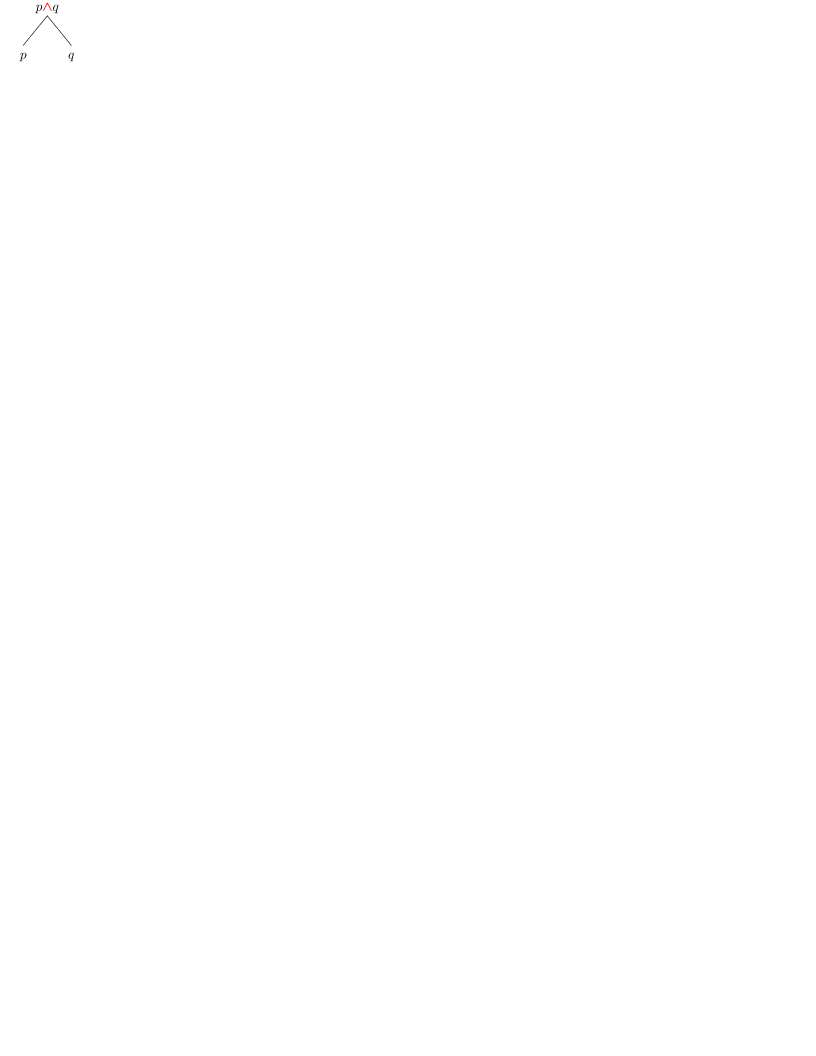
\includegraphics{Tree1}
\end{center}
\end{warpHTML}


To help you more easily see what is going on, the connective which is introduced at each node is in boldface red.

\end{example}

We will later see an algorithm which given a propositional formula allows you to compute a construction tree for it.

\marginpar{{\color{red}End of L1\&L2}}

\subsubsection*{Induction on the complexity of propositional formulas}

We will frequently prove properties of propositional formulas by ``induction on complexity''. To prove a statement about all propositional formulas, using this method of proof, we first prove the statement for $\PF_0\mcal{L}$ (this is our base case) and then show that, for all $n\in\N_0$, if the statement holds of $\PF_n\mcal{L}$ then it also holds for $\PF_{n+1}\mcal{L}$.

Here is a simple first example. Before reading the proof of this lemma, look at the definition of a propositional formula and think about why it is true.
\begin{lemma}\label{leftrightbrackets}
Let $\mcal{L}$ be a propositional language. Suppose $s\in \PF\mcal{L}$. The number of open brackets $($ occuring in $s$ is equal to the number of close brackets $)$ occuring in $s$.
\end{lemma}
\begin{proof}
For any propositional formula $s$, define $l[s]$ (respectively $r[s]$) to be the number of open brackets `` $($ '' (respectively close brackets `` $)$ '') occurring in $s$. If $s\in \PF_0\mcal{L}$ then $s$ is either a propositional variable or $\bot$. So $l[s]=0=r[s]$. Hence the statement of the lemma is true for all $s\in \PF_0\mcal{L}$. For the induction step, suppose that for all $s\in \PF_n\mcal{L}$, $l[s]=r[s]$. Let $t$ be a propositional formula in $\PF_{n+1}\mcal{L}$. Then, examining the definition of $\PF_{n+1}\mcal{L}$, either $t\in \PF_n\mcal{L}$, $t$ is $(\neg s)$ for some $s\in \PF_n\mcal{L}$ or $t$ is $(s_1\square s_2)$ for some propositional formulas $s_1,s_2\in \PF_n\mcal{L}$ and some connective $\square$ of arity $2$.

If $t\in \PF_n\mcal{L}$ then $l[t]=r[t]$ by our induction hypothesis.

If $t$ is $(\neg s)$ then $l[t]=l[(\neg s)]=l[s]+1$ and $r[t]=r[(\neg s)]=r[s]+1$. By the induction hypothesis, $l[s]=r[s]$. Therefore $l[t]=r[t]$.

If $t$ is $(s_1\square s_2)$ for some propositional formulas $s_1,s_2\in \PF_n\mcal{L}$ and some connective $\square$ of arity $2$ then $l[(s_1\square s_2)]=l(s_1)+l(s_2)+1$ and $r[(s_1\square s_2)]=r[s_1]+r[s_2]+1$. By the induction hypothesis $l[s_1]=r[s_1]$ and $l[s_2]=r[s_2]$. Therefore \[l[t]=l[(s_1\square s_2)]=l[s_1]+l[s_2]+1=r[s_1]+r[s_2]+1=r[(s_1\square s_2)]=r[t].\] Thus we have proved the inductive step. Hence the lemma holds by induction on the complexity of propositional formulas.
\end{proof}

%\begin{proof}
%For any propositional formula $s$, define $l(s)$ (respectively $r(s)$) to be the number of open brackets `` $($ '' (respectively close brackets `` $)$ '') occurring in $s$. If $s\in \PF_0\mcal{L}$ then $s$ is either a propositional variable or $\bot$. So $l(s)=0=r(s)$. Hence the statement of the lemma is true for all $s\in \PF_0\mcal{L}$. For the induction step, suppose that for all $s\in \PF_n\mcal{L}$, $l(s)=r(s)$. Let $t$ be a propositional formula in $\PF_{n+1}\mcal{L}$. Then, examining the definition of $\PF_{n+1}\mcal{L}$, either $t\in \PF_n\mcal{L}$, $t$ is $(\neg s)$ for some $s\in \PF_n\mcal{L}$ or $t$ is $(s_1\square s_2)$ for some propositional formulas $s_1,s_2\in \PF_n\mcal{L}$ and some connective $\square$ of arity $2$.
%
%If $t\in \PF_n\mcal{L}$ then $l(t)=r(t)$ by our induction hypothesis.
%
%If $t$ is $(\neg s)$ then $l(t)=l((\neg s))=l(s)+1$ and $r(t)=r((\neg s))=r(s)+1$. By the induction hypothesis, $l(s)=r(s)$. Therefore $l(t)=r(t)$.
%
%If $t$ is $(s_1\square s_2)$ for some propositional formulas $s_1,s_2\in \PF_n\mcal{L}$ and some connective $\square$ of arity $2$ then $l((s_1\square s_2))=l(s_1)+l(s_2)+1$ and $r((s_1\square s_2))=r(s_1)+r(s_2)+1$. By the induction hypothesis $l(s_1)=r(s_1)$ and $l(s_2)=r(s_2)$. Therefore \[l(t)=l((s_1\square s_2))=l(s_1)+l(s_2)+1=r(s_1)+r(s_2)+1=r((s_1\square s_2))=r(t).\] Thus we have proved the inductive step. Hence the lemma holds by induction on the complexity of propositional formulas.
%\end{proof}

We now state a ``meta'' theorem. The reason it is ``meta'' is that we deliberately don't define what we mean by ``property''. It is intended to give a template for what needs to be shown in order to prove something by induction on complexity of formulas.

For a property $X$ of propositional formulas and, in this instance, a propositional formula $t$, we will write $X(t)$ to mean that property $X$ holds for $t$. For example, $X$ could be the property that $t$ has the same number of open brackets as close brackets as in the previous lemma.

\begin{metatheorem}
Let $X$ be a property of propositional formulas and let $\mcal{L}$ be a propositional language. Suppose that the following hold:
\begin{enumerate}
\item For all propositional variables $p$, $X(p)$ and $X(\bot)$.
\item For all $s\in\PF\mcal{L}$, if $X(s)$ then $X((\neg s))$.
\item For all $s_1,s_2\in\PF\mcal{L}$, $X(s_1)$ and $X(s_2)$ implies $X(s_1\wedge s_2)$.
\item For all $s_1,s_2\in\PF\mcal{L}$, $X(s_1)$ and $X(s_2)$ implies $X(s_1\vee s_2)$.
\item For all $s_1,s_2\in\PF\mcal{L}$, $X(s_1)$ and $X(s_2)$ implies $X(s_1\rightarrow s_2)$.
\end{enumerate}

Then $X(t)$ for all $t\in \PF\mcal{L}$.

\end{metatheorem}
%\begin{proof}[Metaproof]
%ADD
%\end{proof}

\subsubsection*{Unique construction}

The next theorem essentially says that every propositional formula has a unique construction tree.

\begin{theorem}[Unique Construction Theorem]\label{UCProp}
For any propositional formula $t$, exactly one of the following is true:
\begin{enumerate}
\item $t$ is a propositional variable.
\item $t$ is $\bot$.
\item $t$ is of the form $(\neg s)$ for a unique propositional formula $s$.
\item $t$ is of the form $(s_1\conn s_2)$ for a unique connective $\conn$ of arity $2$ and a unique pair of propositional formulas $(s_1,s_2)$.
\end{enumerate}
\end{theorem}

Without the ``exactly one'' and ``unique'', the theorem easily follows from the definition of a propositional formula. To deal with the uniqueness part, we need some definitions and a lemma.

\begin{definition}
Let $x$ be a word in a propositional language $\mcal{L}$.
If $x$ is of the form $yz$ for words $y$ and $z$ in $\mcal{L}$ then we call $y$ a \textbf{proper left subword} of $x$. A word is a \textbf{left subword} of $x$ if it is either equal to $x$ or is a proper left subword of $x$.
\end{definition}

\begin{lemma}\label{leftsubwords}
Let $\mcal{L}$ be a propositional language and let $t\in \PF\mcal{L}$. If $w$ is a proper left subword of $t$ then $l(w)<r(w)$ where $l(w)$ denotes the number of open brackets occurring in $w$ and $r(w)$ denotes the number of close brackets occurring in $w$.
\end{lemma}
\begin{proof}
We prove the statement by induction on the complexity of $t$. If $t\in \PF_0\mcal{L}$ then $t$ has no proper left subwords. So the statement is vacuously true. We now prove the induction step. Suppose that the statement is true for propositional formulas in $\PF_i\mcal{L}$. Take $t\in \PF_{i+1}\mcal{L}\backslash \PF_i\mcal{L}$. We now have $2$ cases to consider. If $t$ is $(\neg s)$ for some $s\in \PF_i\mcal{L}$ and $w$ is a proper left subword of $t$ then either $w$ is $($, $(\neg$ or $(\neg y$ where $y$ is a left subword of $s$. It's clear that $l(w)>r(w)$ in the first $2$ cases. So suppose that $t$ is $(\neg y$ for $y$ a left subword of $s$. By the induction hypothesis and \ref{leftrightbrackets}, $l(y)\geq r(y)$. Therefore $l((\neg y)=1+l(y)\geq 1+r(y)>r(y)=r((\neg y)$ as required.

If $t$ is of the form $(s_1\square s_2)$ for $s_1,s_2\in \PF_i\mcal{L}$ and $w$ is a proper left subword of $t$ then either $w$ is $($, $(y$ where $y$ is a left subword of $s_1$, $(s_1\square$ or $(s_1\square z$ where $z$ is a  left subword of $s_2$. If $w$ is $($ then $l(w)=1>0=r(w)$. If $y$ is a left subword of $s_1$ then by the induction hypothesis and \ref{leftrightbrackets}, we know that $l(y)\geq r(y)$. Therefore $l((y)=l(y)+1>r(y)=r((y)$ and $l((y\square)=l(y)+1>r(y)=r((y\square)$ as required. We now suppose that $z$ is a subword of $s_2$. Then $l(z)\leq r(z)$ by \ref{leftrightbrackets} and the induction hypothesis. So
\begin{eqnarray*}
% \nonumber to remove numbering (before each equation)
  l((s_1\square z) &=& 1+l(s_1)+l(z) \\
   &=& 1+ r(s_1)+l(z) \qquad \text{(by \ref{leftrightbrackets})}\\
   &\geq& 1 + r(s_1)+r(z) \\
   &=& 1+ r((s_1\square z) \\
   &>& r((s_1\square z)
\end{eqnarray*} as required.
\end{proof}



For future use we record the following remark.
\begin{remark}\label{startofpropfla}
\begin{enumerate}[(a)]
\item The first letter of any propositional formula is either ``$($'', a propositional variable or $\bot$.
\item All propositional formulas of length $\geq 2$, start as $(\neg$, $(($, $(p$ or $(\bot$ where $p$ is a propositional variable.
\end{enumerate}
\end{remark}
\begin{proof}
(a) Let $t\in\PF\mcal{L}$. If $t\in \PF_0\mcal{L}$ then the first and only letter of $t$ is a propositional variable or $\bot$. Otherwise, it follows directly from the definition of a propositional formula that the first letter of $t$ is $($.

(b) All propositional formulas not in $\PF_0\mcal{L}$ are of the form $(\neg s)$ or $(s_1\conn s_2)$ where $s_1$ and $s_2$ are propositional formulas and $\conn$ is a connective of arity $2$. Formulas of the form $(\neg s)$ are as described by the statement of the lemma, so we just need to consider those of the form $(s_1\conn s_2)$. The second letter of $(s_1\conn s_2)$ is the first letter of $s_1$. The statement now follows from (a).
\end{proof}







We are now ready to prove the Unique Construction Theorem.

\begin{proof}[Proof of the Unique Construction Theorem. ]
It follows from the definition of a propositional formula that each propositional formula is of one of the required forms.

Clearly a propositional formula which satisfies $1$ or $2$ does not satisfy any of the other cases. If a propositional formula satisfies $3$ then its first $2$ letters are $(\neg$. If a propositional formula satisfies $4$ then its first $2$ letters are either $(($, $(p$ or $(\bot$ for $p\in\PROP(\mcal{L})$. Thus no propositional formula can satisfy $3$ and $4$.

We now just need to show the uniqueness in $3$ and $4$. If $t$ is $(\neg s)$ and $(\neg s')$ for propositional formulas $s$ and $s'$. Then clearly $s=s'$. So we consider the case where $t$ is $(s_1\square s_2)$ and $(s_1'\square's_2')$. Then either $s_1$ is a left subword of $s_1'$ or $s_1'$ is a left subword of $s_1$. Without loss of generality, suppose $s_1$ is a left subword of $s_1'$. If $s_1$ is a proper left subword then the number of open brackets of $s_1$ is strictly greater than the number of close brackets of $s_1$. But since $s_1$ is a propositional formula, its number of open brackets is equal to its number of close brackets. Therefore $s_1=s_1'$. It now follows that $\square =\square'$ and then that $s_2=s_2'$ as required.
\end{proof}




\subsubsection*{An algorithm to compute the construction tree of a propositional formula}

When we introduced construction trees we saw the construction tree of the propositional formula $(((p_4\rightarrow (\neg p_1))\wedge p_2)\vee((\neg p_3)\wedge (p_2\rightarrow \bot)))$. Given the construction tree it was reasonably easy to check it was correct and hence confirm that  $(((p_4\rightarrow (\neg p_1))\wedge p_2)\vee((\neg p_3)\wedge (p_2\rightarrow \bot)))$ is indeed a propositional formula. We will now see an algorithm to compute the construction tree of a propositional formula based on the proof of the Unique Construction Theorem.

\bigskip

\noindent
\textbf{Case 0:} If a propositional formula is in $\PF_0\mcal{L}$ then we just write down the formula.

\medskip

For propositional formulas not in $\PF_0\mcal{L}$, we split into $3$ cases suggested by \ref{startofpropfla}.

\medskip

\noindent
\textbf{Case 1:} The first $2$ letters of $t$ are $(\neg$.

In this case $t$ is of the form $(\neg s)$ and the construction tree starts:
\begin{warpprint}
\begin{center}
\synttree[$(\neg s)$[$s$]]
\end{center}
\end{warpprint}
\begin{warpHTML}
\begin{center}
\begin{tikzpicture}
\synttree[$(\neg s)$[$s$]]
\end{tikzpicture}
\end{center}
\end{warpHTML}

To continue, we now just need to find the construction tree of $s$.

\medskip

\noindent
\textbf{Case 2:} The first $2$ letters of $t$ are ``$(p$'' or ``$(\bot$'' for some propositional variable $p$.

In this case $t$ is of the form $(p\conn s)$ or $(\bot \conn s)$ for some propositional formula $s$ and connective $\square$ of arity $2$. So the construction tree starts respectively:
\begin{warpprint}
\begin{center}
\synttree[$(p\conn s)$[$p$][$s$]]\qquad\qquad\synttree[$(\bot \conn s)$[$\bot$][$s$]]
\end{center}
\end{warpprint}
\begin{warpHTML}
\begin{center}
\begin{tikzpicture}
\synttree[$(p\conn s)$[$p$][$s$]]
\end{tikzpicture} \qquad \qquad
\begin{tikzpicture}
\synttree[$(\bot \conn s)$[$\bot$][$s$]]
\end{tikzpicture}
\end{center}
\end{warpHTML}


\noindent
\textbf{Case 3:} The first $2$ letters of $t$ are ``$(($''.

In this case $t$ is of the form $(s_1\conn s_2)$ and the first letter of $s_1$ is $($. So the construction tree of $t$ starts:

\begin{warpprint}
\begin{center}
\synttree[$(s_1\conn s_2)$[$s_1$][$s_2$]]
\end{center}
\end{warpprint}
\begin{warpHTML}
\begin{center}
\begin{tikzpicture}
\synttree[$(s_1\conn s_2)$[$s_1$][$s_2$]]
\end{tikzpicture}
\end{center}
\end{warpHTML}

But how do we find $s_1$, $\conn$ and $s_2$?

Since the first letter of $s_1$ is $($, $s_1$ is not in $\PF_0\mcal{L}$. By \ref{leftsubwords}, for all proper left subwords $y$ of $s$, the number of open brackets in $y$ is strictly less than the number of close brackets in $y$. Thus $s_1$ is the shortest left subword of $s_1\square s_2)$ with equal number of open and close brackets.


Hence, in order to find $s_1$, we \textit{just} need to count open and close brackets in $(s_1\conn s_2)$ to compute the last close bracket in $s_1$.

We number the first (open) bracket in  $(s_1\conn s_2)$ with $1$. We continue from left to right labelling each open bracket with $i+1$ if the previous bracket was labelled $i$ and each close bracket $i-1$ if the previous bracket was labelled $i-1$. We continue until we label a close bracket with a $1$. Then $s_1$ is the formula starting with the open bracket labelled $2$ and ending with the close bracket labelled $1$.

This process is easier to understand once you have seen an example. Consider the propositional formula
\[(((\neg p)\rightarrow ((p\rightarrow(\neg q))\rightarrow(\neg r)))\rightarrow (p\rightarrow r)).\]
Assuming this is indeed a propositional formula, we know that it is the form $(s_1\conn s_2)$ and we want to find $s_1$, $\conn$ and $s_2$. Here is the propositional formula with the brackets numbered:
\[\underset{1}{(}\underset{ 2}{(}\underset{3}{(}\neg p\underset{ 2}{)}\rightarrow \underset{3}{(}\underset{ 4}{(}p\rightarrow\underset{ 5}{(}\neg q\underset{4}{)}\underset{3}{)}\rightarrow \underset{4}{(}\neg r\underset{ 3}{)}\underset{ 2}{)}\underset{ 1}{)}\rightarrow (p\rightarrow r))\]

Here it is with $s_1$ and $s_2$ labelled:
\[\underset{1}{(}\overbrace{\underset{ 2}{(}\underset{3}{(}\neg p\underset{ 2}{)}\rightarrow \underset{3}{(}\underset{ 4}{(}p\rightarrow\underset{ 5}{(}\neg q\underset{4}{)}\underset{3}{)}\rightarrow \underset{4}{(}\neg r\underset{ 3}{)}\underset{ 2}{)}\underset{ 1}{)}}^{s_1}\rightarrow \overbrace{(p\rightarrow r)}^{s_2})\]
%$\underset{(}{1}$

The last connective introduced in the construction of $(s_1\square s_2)$ is $\rightarrow$ i.e. $\square$ is $\rightarrow$ and $s_2$ is
$(p\rightarrow r)$.



So the start of the construction tree is
%\newcount\MTr@branchheight
%\newcommand{\branchheight}[1]{
%\setlength{\MTr@templength}{#1}
%\MTr@branchheight\MTr@templength}
\branchheight{1.5cm}
%%\childsidesep{1em}
\childattachsep{4cm}


\begin{warpprint}
\begin{center}
\synttree[$(((\neg p)\rightarrow ((p\rightarrow(\neg q))\rightarrow(\neg r)))\rightarrow (p\rightarrow r))$[$((\neg p)\rightarrow ((p\rightarrow(\neg q))\rightarrow (\neg r)))$][$(p\rightarrow r)$]]
\end{center}
\end{warpprint}
\begin{warpHTML}
\begin{center}
\begin{tikzpicture}
\synttree[$(((\neg p)\rightarrow ((p\rightarrow(\neg q))\rightarrow(\neg r)))\rightarrow (p\rightarrow r))$[$((\neg p)\rightarrow ((p\rightarrow(\neg q))\rightarrow (\neg r)))$][$(p\rightarrow r)$]]
\end{tikzpicture}
\end{center}
\end{warpHTML}

\marginpar{{\color{gray}End of L3\&L4}}



We will now see a(n almost) full worked example of applying the construction tree algorithm to the propositional formula $(((\neg p)\rightarrow ((p\rightarrow(\neg q))\rightarrow(\neg r)))\rightarrow (p\rightarrow r))$.

\bigskip

\begin{warpprint}
\begin{center}
\synttree[(1)\quad$(((\neg p)\rightarrow ((p\rightarrow(\neg q))\rightarrow(\neg r)))\rightarrow (p\rightarrow r))$ \quad\phantom{(1)}[(2)\quad$((\neg p)\rightarrow ((p\rightarrow(\neg q))\rightarrow (\neg r)))$ \phantom{(2)\quad}[(3)\quad$(\neg p)$\phantom{(3)\quad}[$p$]][(4)\quad $((p\rightarrow(\neg q))\rightarrow (\neg r))$ \phantom{(4)\quad}[(5)\quad$(p\rightarrow (\neg q))$\phantom{(5)\quad}[$p$][(6)\quad$(\neg q)$\phantom{(6)\quad}[$q$]]][(7)\quad$(\neg r)$\phantom{(7)\quad}[$r$]]]][(8)\quad$(p\rightarrow r)$\phantom{(8)\quad}[$p$][$r$]]]
\end{center}
\end{warpprint}
\begin{warpHTML}
REPLACE WITH PDF
\begin{center}
\begin{tikzpicture}
\synttree[(1)\quad$(((\neg p)\rightarrow ((p\rightarrow(\neg q))\rightarrow(\neg r)))\rightarrow (p\rightarrow r))$ \quad\phantom{(1)}[(2)\quad$((\neg p)\rightarrow ((p\rightarrow(\neg q))\rightarrow (\neg r)))$ \phantom{(2)\quad}[(3)\quad$(\neg p)$\phantom{(3)\quad}[$p$]][(4)\quad $((p\rightarrow(\neg q))\rightarrow (\neg r))$ \phantom{(4)\quad}[(5)\quad$(p\rightarrow (\neg q))$\phantom{(5)\quad}[$p$][(6)\quad$(\neg q)$\phantom{(6)\quad}[$q$]]][(7)\quad$(\neg r)$\phantom{(7)\quad}[$r$]]]][(8)\quad$(p\rightarrow r)$\phantom{(8)\quad}[$p$][$r$]]]
\end{tikzpicture}
\end{center}
\end{warpHTML}


\medskip
\noindent
$\bm{(1)}$ The propositional formula $(((\neg p)\rightarrow ((p\rightarrow(\neg q))\rightarrow(\neg r)))\rightarrow (p\rightarrow r))$ starts with $(($ so we apply case $3$ and count the brackets. We've already done this step when describing the algorithm.

\medskip
\noindent
$\bm{(2)}$ The propositional formula $((\neg p)\rightarrow ((p\rightarrow(\neg q))\rightarrow (\neg r)))$ starts with $(($ so we apply case $3$ and count the brackets as follows:
\[\underset{1}{(}\underset{2}{(}\neg p\underset{1}{)}\rightarrow ((p\rightarrow(\neg q))\rightarrow (\neg r)))\]
So we get the construction tree
\begin{warpprint}
\begin{center}
\synttree[$((\neg p)\rightarrow ((p\rightarrow(\neg q))\rightarrow (\neg r)))$[$(\neg p)$][$((p\rightarrow(\neg q))\rightarrow (\neg r))$]]
\end{center}
\end{warpprint}
\begin{warpHTML}
\begin{center}
\begin{tikzpicture}
\synttree[$((\neg p)\rightarrow ((p\rightarrow(\neg q))\rightarrow (\neg r)))$[$(\neg p)$][$((p\rightarrow(\neg q))\rightarrow (\neg r))$]]
\end{tikzpicture}
\end{center}
\end{warpHTML}


\medskip
\noindent
$\bm{(3)}$ The propositional formula $(\neg p)$ starts with $(\neg$ so we apply case $1$ and get the construction tree
\begin{warpprint}
\begin{center}
\synttree[$(\neg p)$[$p$]]
\end{center}
\end{warpprint}
\begin{warpHTML}
\begin{center}
\begin{tikzpicture}
\synttree[$(\neg p)$[$p$]]
\end{tikzpicture}
\end{center}
\end{warpHTML}


\medskip
\noindent
$\bm{(4)}$ The propositional formula $((p\rightarrow(\neg q))\rightarrow (\neg r))$ starts with $(($ so we apply case $3$ and count brackets as follows:
\[\underset{1}{(}\underset{2}{(}p\rightarrow\underset{3}{(}\neg q\underset{2}{)}\underset{1}{)}\rightarrow (\neg r))\]
So we get the construction tree
\begin{warpprint}
\begin{center}
\synttree[$((p\rightarrow(\neg q))\rightarrow (\neg r))$[$(p\rightarrow(\neg q))$][$(\neg r)$]]
\end{center}
\end{warpprint}
\begin{warpHTML}
\begin{center}
\begin{tikzpicture}
\synttree[$((p\rightarrow(\neg q))\rightarrow (\neg r))$[$(p\rightarrow(\neg q))$][$(\neg r)$]]
\end{tikzpicture}
\end{center}
\end{warpHTML}




\medskip
\noindent
$\bm{(5)}$ The propositional formula $(p\rightarrow (\neg q))$ starts with $(p$ and $p$ is a propositional variable so we apply case $2$ and get the construction tree
\begin{warpprint}
\begin{center}
\synttree[$(p\rightarrow (\neg q))$[$p$][$(\neg q)$]]
\end{center}
\end{warpprint}
\begin{warpHTML}
\begin{center}
\begin{tikzpicture}
\synttree[$(p\rightarrow (\neg q))$[$p$][$(\neg q)$]]
\end{tikzpicture}
\end{center}
\end{warpHTML}


\medskip
\noindent
$\bm{(6)}$ and $\bm{(7)}$ are like $\bm{(3)}$.

\medskip
\noindent
$\bm{(8)}$ The propositional formula $(p\rightarrow r)$ starts with $(p$ and $p$ is a propositional variable so we apply case $2$ and get the construction tree
\begin{warpprint}
\begin{center}
\synttree[$(p\rightarrow r)$[$p$][$r$]]
\end{center}
\end{warpprint}
\begin{warpHTML}
\begin{center}
\begin{tikzpicture}
\synttree[$(p\rightarrow r)$[$p$][$r$]]
\end{tikzpicture}
\end{center}
\end{warpHTML}


\begin{remark}
Although I haven't justified this, if the construction tree algorithm goes wrong at any point then the word we started with is not a propositional formula. This roughly follows from the proof of the unique readability theorem. This is important because it means a computer can not only compute construction trees but determine whether a word is a propositional formula or not.
\end{remark}




















%
%\subsubsection*{Construction trees and recognising propositional formulas}
%
%In this subsection we introduce construction trees and present an algorithm for finding the construction tree of a propositional formula. Note that the idea of a construction tree will reappear in the predicate logic section.
%
%Before explaining what a construction tree is, it is helpful to see an example. The following is the construction tree of the propositional formula $(((p_4\rightarrow (\neg p_1))\wedge p_2)\vee((\neg p_3)\wedge (p_2\rightarrow \bot)))$:
%
%\medskip
%\begin{center}
%\synttree[$(((p_4\rightarrow (\neg p_1))\wedge p_2)\bm{{\color{red}\vee}}((\neg p_3)\wedge (p_2\rightarrow \bot)))$[$((p_4\rightarrow (\neg p_1))\bm{{\color{red}\wedge}} p_2)$[$(p_4\bm{{\color{red}\rightarrow}} (\neg p_1))$[$p_4$][$(\bm{{\color{red}\neg }}p_1)$[$p_1$]]][$p_2$]][$((\neg p_3)\bm{{\color{red}\wedge }}(p_2\rightarrow \bot))$[$(\bm{{\color{red}\neg}} p_3)$[$p_3$]][$(p_2\bm{{\color{red}\rightarrow}} \bot)$[$p_2$][$\bot$]]]]\\
%\end{center}
%
%To help you more easily see what is going on, the connective which is introduced at each node is in boldface red.
%
%
%%\begin{center}
%%\synttree[$(((p_4\rightarrow (\neg p_1))\wedge p_2)\bm{\vee}((\neg p_3)\wedge (p_2\rightarrow \bot)))$[$((p_4\rightarrow (\neg p_1))\bm{\wedge} p_2)$[$(p_4\bm{\rightarrow} (\neg p_1))$[$p_4$][$(\bm{\neg }p_1)$[$p_1$]]][$p_2$]][$((\neg p_3)\bm{\wedge }(p_2\rightarrow \bot))$[$(\bm{\neg} p_3)$[$p_3$]][$(p_2\bm{\rightarrow} \bot)$[$p_2$][$\bot$]]]]\\
%%\end{center}
%
%%\begin{center}
%%\synttree[$(((p_4\rightarrow (\neg p_1))\wedge p_2){\color{red}\vee}((\neg p_3)\wedge (p_2\rightarrow \bot)))$[$((p_4\rightarrow (\neg p_1)){\color{red}\wedge} p_2)$[$(p_4{\color{red}\rightarrow} (\neg p_1))$[$p_4$][$({\color{red}\neg }p_1)$[$p_1$]]][$p_2$]][$((\neg p_3){\color{red}\wedge }(p_2\rightarrow \bot))$[$({\color{red}\neg} p_3)$[$p_3$]][$(p_2{\color{red}\rightarrow} \bot)$[$p_2$][$\bot$]]]]\\
%%\end{center}
%
%
%Particularly if you are doing the combinatorics course, note that these are not quite trees in the usual sense because we distinguish between left and right branches. Formally we are talking about
%
%\bigskip
%
%\noindent
%\textbf{An algorithm for finding the construction tree of a propositional formula.}
%
%
%
%
%If a propositional formula is in $\PF_0\mcal{L}$ (or equivalently has length $1$)then it has just one node which is labelled with the formula itself. For instance the construction tree of $p$ where $p$ is a proposition is:
%\begin{center}
%\synttree[$p$]
%\end{center}
%
%For propositional formulas not in $\PF_0\mcal{L}$, we split into $3$ cases suggested by \ref{startofpropfla}.
%
%\noindent
%\textbf{Case 1:} The first $2$ letter of $F$ are $(\con$ where $\con$ is a connective of arity $1$.
%
%In this case $F$ is of the form $(\con G)$ and the construction tree starts:
%
%\begin{center}
%\synttree[$(\con G)$[$G$]]
%\end{center}
%
%To continue, we now just need to find the construction tree of $G$.
%
%\noindent
%\textbf{Case 2:} The first $2$ letters of $F$ are ``$(p$'' or ``$(\bot$'' for some propositional variable $p$ and logical constant $\bot$.
%
%In this case $F$ is of the form $(p\conn G)$ or $(\bot \conn G)$ for some propositional formula $G$ and connective of arity $2$. So the construction starts respectively:
%\begin{center}
%\synttree[$(p\conn G)$[$p$][$G$]]\qquad\qquad\synttree[$(\bot \conn G)$[$\bot$][$G$]]
%\end{center}
%\noindent
%\textbf{Case 3:} The first $2$ letters of $F$ are ``$(($''.
%
%In this case $F$ is of the form $(A\conn B)$ and the first letter of $A$ is $($. So the construction tree of $F$ starts:
%
%\begin{center}
%\synttree[$(A\conn B)$[$A$][$B$]]
%\end{center}
%
%But how do we find $A$, $\conn$ and $B$?
%
%Since the first letter of $A$ is $($, $A$ is not in $\PF_0\mcal{L}$. Since the number of open brackets in $A$ must be equal to the number of close brackets in $A$, to find $\conn$ we just need to count open and close brackets in $(A\conn B)$ to the last close bracket in $A$.
%
%We number the first (open) bracket in  $(A\conn B)$ with $1$. We continue until label a close bracket with a $1$.
%
%This process is easier to understand once you have seen an example. Consider the propositional formula
%\[(((\neg p)\rightarrow ((p\rightarrow(\neg q))\rightarrow(\neg r)))\rightarrow (p\rightarrow r)).\]
%Assuming this is indeed a propositional formula, we know that it is the form $(A\conn B)$ and we want to find $A$, $\conn$ and $B$. Here is the propositional formula with the brackets numbered:
%\[\underset{1}{(}\underset{ 2}{(}\underset{3}{(}\neg p\underset{ 2}{)}\rightarrow \underset{3}{(}\underset{ 4}{(}p\rightarrow\underset{ 5}{(}\neg q\underset{4}{)}\underset{3}{)}\rightarrow \underset{4}{(}\neg r\underset{ 3}{)}\underset{ 2}{)}\underset{ 1}{)}\rightarrow (p\rightarrow r))\]
%
%\[\underset{1}{(}\overbrace{\underset{ 2}{(}\underset{3}{(}\neg p\underset{ 2}{)}\rightarrow \underset{3}{(}\underset{ 4}{(}p\rightarrow\underset{ 5}{(}\neg q\underset{4}{)}\underset{3}{)}\rightarrow \underset{4}{(}\neg r\underset{ 3}{)}\underset{ 2}{)}\underset{ 1}{)}}^{A}\rightarrow \overbrace{(p\rightarrow r)}^B)\]
%%$\underset{(}{1}$
%
%The last connective introduced in the construction of $(A\square B)$ is $\rightarrow$ i.e. $\square$ is $\rightarrow$ and $B$ is
%$(p\rightarrow r)$.
%
%So the start of the construction tree is
%%\newcount\MTr@branchheight
%%\newcommand{\branchheight}[1]{
%%\setlength{\MTr@templength}{#1}
%%\MTr@branchheight\MTr@templength}
%\branchheight{1.5cm}
%%\childsidesep{1em}
%\childattachsep{4cm}
%
%\begin{center}
%\synttree[$(((\neg p)\rightarrow ((p\rightarrow(\neg q))\rightarrow(\neg r)))\rightarrow (p\rightarrow r))$[$((\neg p)\rightarrow ((p\rightarrow(\neg q))\rightarrow (\neg r)))$][$(p\rightarrow r)$]]
%\end{center}
%%\[
%%((\neg p)\rightarrow ((p\rightarrow(\neg q))\rightarrow (\neg r)))\]
%%
%%\[\underset{ 2}{(}\underset{3}{(}\neg p\underset{ 2}{)}\rightarrow \underset{3}{(}\underset{ 4}{(}p\rightarrow\underset{ 5}{(}\neg q\underset{4}{)}\underset{3}{)}\rightarrow \underset{4}{(}\neg r\underset{ 3}{)}\underset{ 2}{)}\underset{ 1}{)}.\] The last connective introduced in the construction of $(A\square B)$ is $\rightarrow$ i.e. $\square$ is $\rightarrow$ and $B$ is
%%$(p\rightarrow r)$.
%
%We now do a worked example with all computation shown.
%
%\noindent
%\textbf{STEP 1} The formula starts $(($ so we need to number the brackets.
%\begin{center}
%\synttree[$(((\neg p)\rightarrow ((p\rightarrow(\neg q))\rightarrow(\neg r)))\rightarrow (p\rightarrow r))$[$((\neg p)\rightarrow ((p\rightarrow(\neg q))\rightarrow (\neg r)))$][$(p\rightarrow r)$]]
%\end{center}
%
%We now need to take one of the $2$ leaves of the tree and find their construction tree. I pick the left hand leaf.
%
%\noindent
%\textbf{STEP 2} The formula starts $(($ so we need to number the brackets as follows:
%\[\underset{1}{(}\underset{2}{(}\neg p\underset{1}{)}\rightarrow ((p\rightarrow(\neg q))\rightarrow (\neg r)))\]
%So the construction tree so far is
%\begin{center}
%\synttree[(1)\quad$(((\neg p)\rightarrow ((p\rightarrow(\neg q))\rightarrow(\neg r)))\rightarrow (p\rightarrow r))$ \quad\phantom{(1)}[(2)\quad$((\neg p)\rightarrow ((p\rightarrow(\neg q))\rightarrow (\neg r)))$ \phantom{(2)\quad}[(3)\quad$(\neg p)$\phantom{(3)\quad}[$p$]][(4)\quad $((p\rightarrow(\neg q))\rightarrow (\neg r))$ \phantom{(4)\quad}[(5)\quad$(p\rightarrow (\neg q))$\phantom{(5)\quad}[$p$][(6)\quad$(\neg q)$\phantom{(6)\quad}[$q$]]][(7)\quad$(\neg r)$\phantom{(7)\quad}[$r$]]]][(8)\quad$(p\rightarrow r)$\phantom{(8)\quad}[$p$][$r$]]]
%\end{center}
%
%
%




\subsection{Truth}\label{truth}
The truth of the statement ``$5$ is an odd number and $7$ is prime'' does not really depend on exactly the statements ``$5$ is an odd number'' and ``$7$ is prime''. What is important is that both ``$5$ is an odd number'' and is true ``$7$ is prime'' are true statements.

The truth of a propositional formula should only depend on the truth of the propositional variables it is made up from. Although we have not formally assigned any meaning to connectives, the names we have given indicate what meaning we might want them to have.

In the following definition the symbol $\T$ represents ``true'' and $\F$ represents ``false''. We think of the valuation $v$ as telling us which propositional formulas are true and which are false according to $v$.

%
%The truth of the statement ``$5$ is an odd number and $7$ is prime'' does not really depend on exactly the statements ``$5$ is an odd number'' and ``$7$ is prime''. What is important is that both ``$5$ is an odd number'' and is true ``$7$ is prime'' are true statements.
%
%The truth of a propositional formula should only depend on the truth of the propositional variables it is made up from. Although we have not formally assigned any meaning to connectives, the names we have given indicate what meaning we might want them to have.
%
%%\begin{definition}
%%A truth assignment is a function $v_0:\PROP\rightarrow \{\T,\F\}$.
%%\end{definition}
%
%FINISH
%
%Given a truth assignment, we want to extend it to all propositional formulas. Before we make precise what we mean by this and show that it is possible, we informally discuss how we should treat each of the connectives.
%
%The least controversial connectives are $\wedge$ (and) and $\neg$ (not). We have already discussed $\wedge$ (and). I hope you agree that if a statement is true then its negation should be false and conversely if a statement is false then its negation should be true. For example the statement ``All mathematicians are female'' is false and so its negation ``Not all mathematicians are female'' is true.
%
%We now discuss ``$\vee$'' (or). In everyday life ``or'' is often treated a exclusive. This give rise to the following (not funny) mathematician's/logician's joke:
%
%\begin{dialogue}
%\speak{Unsuspecting member of the non-mathematical population} Would you like a cup of coffee or a cup of tea?
%\speak{Mathematician/Logician} Yes, please.
%\end{dialogue}
%
%
%In mathematics, ``or'' is usually meant non-exclusively.
%
%The connective whose truth definition causes the most confusion is $\rightarrow$ (implication).
%
%The first isomorphism theorem for groups implies the intermediate value theorem (for continuous functions).



\begin{definition}
A \textbf{valuation} is a function $v:\PF\mcal{L}\rightarrow \{\T,\F\}$ which satisfies the following properties for all $s,t\in \PF\mcal{L}$:
\begin{enumerate}
\item $v(\bot)=\F$
\item $v((\neg s))=\left\{
                   \begin{array}{ll}
                     \F, & \hbox{if $v(s)=\T$;} \\
                     \T, & \hbox{otherwise.}
                   \end{array}
                 \right.
$
\item $v((t\wedge s))=\left\{
                      \begin{array}{ll}
                        \T, & \hbox{if $v(t)=\T$ and $v(s)=\T$;} \\
                        \F, & \hbox{otherwise.}
                      \end{array}
                    \right.
$
\item $v((t\vee s))=\left\{
        \begin{array}{ll}
          \F, & \hbox{if $v(s)=\F$ and $v(t)=\F$;} \\
          \T, & \hbox{otherwise.}
        \end{array}
      \right.
$
\item $v((s\rightarrow t))=\left\{
                           \begin{array}{ll}
                             \F, & \hbox{$v(s)=\T$ and $v(t)=\F$;} \\
                             \T, & \hbox{otherwise.}
                           \end{array}
                         \right.
$

\end{enumerate}

We say that a propositional formula $s\in\PF\mcal{L}$ is \textbf{true (respectively false) under the valuation} $v$ if $v(s)=\T$ (respectively if $v(s)=\F$).
\end{definition}

The least controversial parts of this definition are for the connectives are $\wedge$ (and) and $\neg$ (not). We have already discussed $\wedge$ (and). I hope you agree that if a statement is true then its negation should be false and conversely if a statement is false then its negation should be true. For example the statement ``All mathematicians are female'' is false and so its negation ``Not all mathematicians are female'' is true.

We now discuss ``$\vee$'' (or). In everyday life ``or'' is often treated a exclusive. However, in mathematics, ``or'' is usually meant non-exclusively. This give rise to the following (not funny) mathematician's/logician's joke:

\begin{dialogue}
\speak{Unsuspecting member of the non-mathematical population} Would you like a cup of coffee or a cup of tea?
\speak{Mathematician/Logician} Yes, please.
\end{dialogue}

The most controversial part of this definition is the condition for $\rightarrow$ (implies).  As with ``or'' we could just say this is our convention, get used to it. Since our intention is to give a formal definition of truth, this would be a bit unsatisfactory. First note that this definition does not match up with informal speech even amongst mathematicians. For instance, if I claimed that
\begin{center}
``The first isomorphism theorem for groups implies the intermediate value theorem (for continuous functions).''
\end{center}
 many of my colleagues and your lecturers would reasonably disagree.  On the other hand, most of us would accept that
\begin{center}
``If $n=1$ then $(n-1)(n-2)=0$''
\end{center}
 is true for all $n\in\N$. Although we are not yet studying a logic with quantifiers, it becomes clear that the rule for implication must be as we have defined it when we consider statements involving universal quantification (i.e. ``for all'' statements) like the following.
\[\forall\, x ((x>3)\rightarrow (x^2>3))\]
This statement is true if for each $r\in \R$, the statement ``$((r>3)\rightarrow (r^2>3))$'' is true. If we set $r=1$ then $(r>3)$ is false and $r^2>3$ is false. If we set $r=2$ then $r>3$ is false and $r^2>3$ is true. If we set $r=4$ then $r>3$ is true and $r^2>3$ is also true.

\begin{proposition}
Let $\mcal{L}$ be a propositional language.
\begin{enumerate}[(i)]
\item If $w:\PROP(\mcal{L})\rightarrow \{\T,\F\}$ is any function then there is a unique valuation $\PF\mcal{L}\rightarrow \{\T,\F\}$ such that $v(p)=w(p)$ for all $p\in\PROP(\mcal{L})$.
\item If $t\in \PF\mcal{L}$ and $v,w$ are valuations which agree on all of the propositional variables occurring in $t$ then $v(t)=w(t)$.
\end{enumerate}
\end{proposition}
\begin{proof}[Sketch proof]
(i) Let $w:\PROP(\mcal{L})\rightarrow \{\T,\F\}$. For each $i\in \N_0$, we define $v_i:\PF_i\mcal{L}\rightarrow \{\T,\F\}$, by induction on $i$, which satisfies properties $1$-$5$ of the definition of a valuation and such that $v_i(p)=w(p)$ for all $p\in\PROP(\mcal{L})$. For each $i\in\N_0$, $v_{i+1}$ will be the unique such function extending $v_i$.

We define $v_0$ by setting $v_0(p)=w(p)$ for all $p\in\PROP(\mcal{L})$. In order that $v_0$ satisfies $1$-$5$, we must define $v_0(\bot)=\F$.

Suppose we have already defined $v_i:\PF_i\mcal{L}\rightarrow \{\T,\F\}$. Each element of $\PF_{i+1}\mcal{L}$ is either in $\PF_i\mcal{L}$ or is of the form $(\neg s)$ or $(s_1\conn s_2)$ for some $s, s_1,s_2\in \PF_i\mcal{L}$ and connective  $\conn$ of arity $2$. For each connective extend $v_i$ according to the rules for that connective given in the definition of a valuation. For instance, if $t=(\neg s)$ then define $v_{i+1}(t)=\F$ if $v_i(s)=\T$ and define $v_{i+1}(t)=\T$ if $v_i(s)=\F$. The function $v_{i+1}$ is well-defined thanks to the Unique Construction Theorem. Moreover $v_{i+1}$ is the unique function defined on $\PF_{i+1}\mcal{L}$ satisfying $1$-$5$ of the definition of a valuation. Let $v:\PF\mcal{L}\rightarrow \{\T,\F\}$ be defined by $v(s)=v_i(s)$ for each $s\in\PF_i\mcal{L}$. Then $v$ satisfies $1$-$5$ of the definition of a valuation because each $v_i$ does. Moreover it is the unique valuation extending $w$ because each $v_i$ is the unique function defined on $\PF_i\mcal{L}$ which satisfies $1$-$5$ and extends $w$.
\medskip


\noindent
(ii) This is left as an exercise.
\end{proof}



The rules for valuations are displayed in the following two (truth) tables:

\begin{center}
\begin{tabular}{|c||c|}
  \hline
  % after \\: \hline or \cline{col1-col2} \cline{col3-col4} ...
  $p$ & $(\neg p)$ \\\hline
  $\T$ & $\F$ \\
$\F$ & $\T$ \\
  \hline
\end{tabular}
\qquad \qquad
\begin{tabular}{|c|c||c|c|c|}
  \hline
  % after \\: \hline or \cline{col1-col2} \cline{col3-col4} ...
  $p$ & $q$ & $p\wedge q$ & $p\vee q$ & $p\rightarrow q$ \\\hline
  $\T$ & $\T$ & $\T$ & $\T$ & $\T$ \\
  $\T$ & $\F$ & $\F$ & $\T$ & $\F$ \\
  $\F$ & $\T$ &  $\F$ & $\T$ & $\T$ \\
$\F$ & $\F$ &  $\F$ & $\F$ & $\T$ \\
  \hline
\end{tabular}
\end{center}

We have seen that if $s\in \PF\mcal{L}$ and $v$ is a valuation on $\PF\mcal{L}$ then the value of $v(s)$ only depends on the value of $v(p)$ for propositional variables which occur in $s$ (i.e. are letters of $s$).

Suppose that the propositional variables which occur in $s\in\PF\mcal{L}$ are $p_1,\ldots,p_n$. A \textbf{truth table} for $s$ is a table with columns headed $p_1, p_2,\ldots,p_n, s$. If we ignore the column headed $s$ then the rows of the table display all possible configurations of $\T$ and $\F$. The entry of each row of the column labelled $s$ displays the value of $v(s)$ for a valuation with $v(p_i)$ equal to the $i$th entry of that row.

Here is an example of a truth table.

\begin{example}
\
\smallskip

\begin{tabular}{|c|c|c||c|}
  \hline
  % after \\: \hline or \cline{col1-col2} \cline{col3-col4} ...
  $p_1$ & $p_2$ & $p_3$ &  $(p_1\rightarrow (p_2\wedge p_3))$ \\\hline
  $\T$ & $\T$ & $\T$ & $\T$ \\
  $\T$ & $\T$ & $\F$ & $\F$ \\
  $\T$ & $\F$ & $\T$ & $\T$ \\
  $\T$ & $\F$ & $\F$ & $\F$ \\
  $\F$ & $\T$ & $\T$ & $\T$ \\
  $\F$ & $\T$ & $\F$ & $\T$ \\
  $\F$ & $\F$ & $\T$ & $\T$ \\
  $\F$ & $\F$ & $\F$ & $\T$ \\
  \hline
\end{tabular}


\end{example}


\begin{definition}
A propositional formula $t$ is called a \textbf{tautology} if $v(t)=\T$ for all valuations $v$ and \textbf{unsatisfiable} if $v(t)=\F$ for all valuations $v$.
\end{definition}

\begin{remark}
To check if a propositional formula $t$ is a tautology we just need to check that $v(t)=\T$ for valuations on the language with propositional variables occurring in $t$.

For examples, to check if $((p_1\vee (\neg p_1))\vee p_2)$ is a tautology, we only need to consider valuations on $\PF\mcal{L}'$ where $\mcal{L}'$ is the propositional language with $\PROP(\mcal{L}')=\{p_1,p_2\}$.
\end{remark}

\marginpar{{\color{red}End of L5\&L6}}

%We can check if propositional formulas are tautologies using truth tables. Here is an example.
%
%\begin{example}\label{exax1}
%The truth table below shows that the propositional formula $(s\rightarrow (t\rightarrow s))$ is a tautology for any propositional formulas $s$ and $t$.
%
%\begin{tabular}{|c|c||c|c|}
%  \hline
%  % after \\: \hline or \cline{col1-col2} \cline{col3-col4} ...
%   $s$ & $t$ & $(t\rightarrow s)$ & $(s\rightarrow (t\rightarrow s))$ \\\hline
%  $\T$ & $\T$ & $\T$ & $\T$ \\
%  $\T$ & $\F$ & $\T$ & $\T$ \\
%  $\F$ & $\T$ & $\F$ & $\T$ \\
%  $\F$ & $\F$ & $\T$ & $\T$ \\
%  \hline
%\end{tabular}
%\end{example}

A propositional formula $s$ is a tautology if the column in its truth table headed $s$ has all entries $\T$. We give a few tautologies which will be important for the proof system we will introduce in the next section.
\begin{proposition}\label{axiomsaretaut}
For all propositional formulas $r, s$ and $t$, the following propositional formulas are tautologies.
\begin{enumerate}[(i)]
\item $(s\rightarrow (t\rightarrow s))$
\item $((s\rightarrow (t\rightarrow r))\rightarrow ((s\rightarrow t)\rightarrow (s\rightarrow r)))$
\item $((\neg(\neg s))\rightarrow s)$
\end{enumerate}
\end{proposition}
\begin{proof}(i) The following truth table shows that the propositional formula $(s\rightarrow (t\rightarrow s))$ is a tautology for any propositional formulas $s$ and $t$.

\medskip
\begin{tabular}{|c|c||c|c|}
  \hline
  % after \\: \hline or \cline{col1-col2} \cline{col3-col4} ...
   $s$ & $t$ & $(t\rightarrow s)$ & $(s\rightarrow (t\rightarrow s))$ \\\hline
  $\T$ & $\T$ & $\T$ & $\T$ \\
  $\T$ & $\F$ & $\T$ & $\T$ \\
  $\F$ & $\T$ & $\F$ & $\T$ \\
  $\F$ & $\F$ & $\T$ & $\T$ \\
  \hline
\end{tabular}

\medskip

\noindent
(ii) This is on your exercise sheet.

\noindent
(iii) The following truth table shows that $((\neg(\neg s))\rightarrow s)$ is a tautology.

\begin{tabular}{|c||c|c|c|}
  \hline
  % after \\: \hline or \cline{col1-col2} \cline{col3-col4} ...
$s$	&$(\neg s)$	&$(\neg(\neg s))$	& $((\neg(\neg s))\rightarrow s)$\\\hline
$\T$&	$\F$&	$\T$&	$\T$\\
$\F$&	$\T$&	$\F$&	$\T$\\
  \hline
\end{tabular}
\end{proof}

We introduce a useful abbreviation.

\begin{definition}
For all propositional formulas $t$ and $s$, define $(t\leftrightarrow s)$ to be the propositional formula $((t\rightarrow s)\wedge (s\rightarrow t))$. We call the symbol $\leftrightarrow$ biimplication.
\end{definition}

\begin{remark}\

\begin{itemize}
\item
For all propositional formulas $t$ and $s$,

$v((t\leftrightarrow s))=\left\{
                     \begin{array}{ll}
                       \T, & \hbox{if $v(t)=v(s)$;} \\
                       \F, & \hbox{otherwise.}
                     \end{array}
                   \right.
$
\item If $s,t$ are propositional formulas of complexity $l$ and $m$ respectively then the complexity of $(t\leftrightarrow s)$ is $\max\{l,m\}+2$.
\end{itemize}
\end{remark}





\begin{definition}
Let $\mcal{L}$ be a propositional language, let $t\in \PF\mcal{L}$ and let $S\subseteq \PF\mcal{L}$. We write $S\models t$ and say $S$ \textbf{logically implies} $t$ (or $t$ \textbf{is a logical consequence of} $S$) if $v(t)=\T$ for all valuations $v$ such that $v(s)=\T$ for all $s\in S$.
\end{definition}

If $S\subseteq \PF\mcal{L}$ and $t_1,\ldots,t_n,u\in\PF\mcal{L}$ then we, abuse notation and, write $S,t_1,\ldots,t_n\models u$ instead of $S\cup\{t_1,\ldots,t_n\}\models u$ and $t_1,\ldots,t_n\models u$ instead of $\{t_1,\ldots,t_n\}\models u$. Under this convention, $\models u$ means $u$ is a tautology.


\begin{example} For a set of propositional formulas $S$,
$S\models \bot$ means that there are no valuations for which $v(s)=\T$ for all $s\in S$.
\end{example}

\begin{remark}\label{modimp}
If $S\models t$ and $S\models (t\rightarrow u)$ then $S\models u$.
\end{remark}
\begin{proof} Suppose $S\models t$ and $S\models (t\rightarrow u)$.
Let $v$ be a valuation such that $v(s)=\T$ for all $s\in S$. So $v(t)=\T$ and $v(t\rightarrow u)=\T$. If $v(u)=\F$ then, since $v(t)=\T$, $v(t\rightarrow u)=\F$ which contradicts our assumptions. Therefore $v(u)=\T$.
\end{proof}

\begin{definition}
We say propositional formulas $s$ and $t$ are \textbf{logically equivalent}, and write $s\equiv t$, if $v(s)=v(t)$ for all valuations $v$.
\end{definition}

\begin{remark}
For a propositional language $\mcal{L}$, the relation $\equiv$ is an equivalence relation on $\PF\mcal{L}$.
\end{remark}

\begin{lemma}
For propositional formulas $r,s,t$, the following logical equivalences hold.
\begin{enumerate}
\item $(\neg s)\equiv (s\rightarrow \bot)$
\item $(s\vee t)\equiv ((\neg s)\rightarrow t)\equiv ((s\rightarrow \bot)\rightarrow t)$
\item $(s\wedge t)\equiv (\neg(s\rightarrow (\neg t)))$
\item $(s\wedge t)\equiv (t\wedge s)$
\item $(s\vee t)\equiv (t\vee s)$
\item $(\neg(s\wedge t))\equiv ((\neg s)\vee (\neg t))$
\item $(s\wedge t)\equiv (\neg((\neg s)\vee (\neg t)))$
\item $((r\wedge s)\wedge t)\equiv (r\wedge(s\wedge t))$
\item $((r\vee s)\vee t)\equiv (r\vee(s\vee t))$
\end{enumerate}
\end{lemma}
\begin{proof}
These equivalences can be checked using truth tables. Here is an example.

\medskip

\begin{tabular}{|c|c||c|c|}
  \hline
  % after \\: \hline or \cline{col1-col2} \cline{col3-col4} ...
  $s$ & $t$ & $(s\vee t)$ & $(t\vee s)$ \\ \hline\hline
  $\T$ & $\T$ & $\T$ &  $\T$ \\ \hline
  $\T$ & $\F$ &  $\T$ & $\T$ \\ \hline
  $\F$ &  $\T$ &  $\T$ & $\T$ \\ \hline
  $\F$ & $\F$ & $\F$ & $\F$ \\
  \hline
\end{tabular}

\medskip

We see that $(s\vee t)\equiv (t\vee s)$ because the column headed $(s\vee t)$ and the column headed $(t\vee s)$ are equal.

\end{proof}


\begin{lemma}
Suppose that $s,t\in\PF\mcal{L}$. The following are equivalent.
\begin{enumerate}
\item $s\equiv t$;
\item $s\models t$ and $t\models s$;
\item $\models s\leftrightarrow t$; and
\item $s\leftrightarrow t$ is a tautology.
\end{enumerate}
\end{lemma}
\begin{proof}
Exercise (mainly in remembering definitions).
\end{proof}



\subsection*{Normal Forms}

We introduce some useful notation defined by induction. Define $\bigwedge_{i=1}^1 s_1$ to be $s_1$ and $\bigvee_{i=1}^1s_1$ to be $s_1$. For $k\in \N$, we define
\[\bigwedge_{i=1}^{k+1}s_i \quad\text{ to be }\quad (\left(\bigwedge_{i=1}^{k}s_i\right)\wedge s_{k+1}) \qquad\text{ and }\qquad \bigvee_{i=1}^{k+1}s_i \quad\text{ to be }\quad (\left(\bigvee_{i=1}^{k}s_i\right)\vee s_{k+1}).\]

We record how these new symbols behave with respect to valuations and logical equivalence.

\begin{lemma}
Let $s_1,\ldots, s_n\in\PF\mcal{L}$ and let $v:\PF\mcal{L}\rightarrow \{\T,\F\}$ be a valuation. Then
\begin{enumerate}
\item $v(\bigwedge_{i=1}^ns_i)=\T$ if and only if $v(s_i)=\T$ for all $i=1,\ldots,n$;
\item $v(\bigvee_{i=1}^ns_i)=\T$ if and only if $v(s_i)=\T$ for some $i=1,\ldots,n$;
\item $\bigwedge_{i=1}^ns_i\equiv (\neg\bigvee_{i=1}^n (\neg s_i))$; and
\item $\bigvee_{i=1}^ns_i\equiv (\neg\bigwedge_{i=1}^n (\neg s_i))$.
\end{enumerate}
\end{lemma}
\begin{proof}
Each statement is proved by induction on $n$. I will prove the first statement. For $n=1$ the statement is trivial since $\bigwedge_{i=1}^1s_i$ is $s_1$. Suppose the statement is true for $n$. Then $\bigwedge_{i=1}^{n+1}s_i$ is $((\bigwedge_{i=1}^ns_i)\wedge s_{n+1})$. So $v(\bigwedge_{i=1}^{n+1}s_i)=\T$ if and only if $v(\bigwedge_{i=1}^ns_i)=\T$ and $v(s_{i+1})=\T$. By the induction hypothesis, this holds if and only if $v(s_i)=\T$ for all $1\leq i\leq n$ and $v(s_{n+1})=\T$ as required.
\end{proof}

This gives a corollary.
\begin{cor}If $s_1,\ldots, s_n\in \PF\mcal{L}$ and $t_1,\ldots,t_m\in \PF\mcal{L}$ are such that $\{s_1,\ldots,s_n\}=\{t_1,\ldots,t_m\}$ then
\[\bigwedge_{i=1}^ns_i\equiv \bigwedge_{i=1}^mt_i\] and
\[\bigvee_{i=1}^ns_i\equiv \bigvee_{i=1}^mt_i\]
\end{cor}

\begin{definition}
A propositional formula is in \textbf{disjunctive normal form (DNF)} if it is of the form $\bot$, $(\neg\bot)$ or
\[\bigvee_{i=1}^l\bigwedge_{j=1}^{m_i} g_{ij}\] where each $g_{ij}$ is either a propositional variable or the negation of a propositional variable.
%
%We say a propositional formula of the form
%\[\bigvee_{i=1}^l\bigwedge_{j=1}^{m_i} g_{ij}\] is in \textbf{disjunctive normal form (DNF)} when each $g_{ij}$ is either a propositional variable or the negation of a propositional variable.
\end{definition}


\begin{theorem}[The disjunctive normal form theorem]
If $t$ is a propositional formula then there exists a propositional formula $s$ in DNF such that $t\equiv s$. Moreover, assuming some propositional variables occur in $t$, if $\{p_1,\ldots,p_n\}$ are the propositional variables occurring in $t$ then we can pick $s$ of the form
\[\bigvee_{i=1}^l\bigwedge_{j=1}^{m_i} g_{ij}\]
where $l\leq 2^n$, $m_i\leq n+1$ and each $g_{ij}$ is of the form $p_k$ or $(\neg p_k)$ for $1\leq k\leq n$.
\end{theorem}
\begin{proof}
If there are no propositional variables occurring in $t$ then either $t\equiv \bot$ or $t\equiv (\neg\bot)$.

Suppose the propositional variables occurring in $t$ are $\{p_1,\ldots,p_n\}$. If $t$ is unsatisfiable then $t\equiv (p_1\wedge (\neg p_1))$. Suppose $t$ is not unsatisfiable. Let $v_1,\ldots, v_l$ be the valuations on $\PF\mcal{L}$ where $\PROP(\mcal{L})=\{p_1,\ldots p_n\}$ such that $v_i(t)=\T$. For each $i=1,\ldots,l$ and $j=1,\ldots, n$, define
\[g_{ij}=\left\{
           \begin{array}{ll}
             p_j, & \hbox{if $v_i(p_j)=\T$;} \\
             (\neg p_j), & \hbox{if $v_i(p_j)=\F$.}
           \end{array}
         \right.
\]

\marginpar{{\color{gray}End of L7 \& L8}}
Let $v$ be any valuation on $\PF\mcal{L}$.
Then $v(\bigwedge_{j=1}^{n} g_{ij})=\T$ if and only if $v=v_i$. Therefore $v(\bigvee_{i=1}^l\bigwedge_{j=1}^{n} g_{ij})=\T$ if and only if $v=v_i$ for some $1\leq i\leq l$. Thus $\bigvee_{i=1}^l\bigwedge_{j=1}^{n} g_{ij}$ is of the required form and logically equivalent to $t$. We see that $l\leq 2^n$ because the number of valuations on $\PF\mcal{L}$ is $2^n$.
\end{proof}

This proof gives a method to find a propositional formula in DNF which is equivalent to a given formula. There is an exercise on your exercise sheet which asks you to do this in a few examples.


\subsubsection*{Adequate sets of connectives}

In this subsection we need to expand our definition of a connective. Initially, in \ref{propflas}, they were a set of $5$ symbols $\{\bot, \neg, \wedge, \vee, \rightarrow\}$ each of which has an associated number in $\{0,1,2\}$ called the arity of the connective which determined how they could be used to form propositional formulas. At this point, apart from what they look like as symbols and what we called them, there was no real difference between $\wedge, \vee$ and $\rightarrow$. In \ref{truth}, we differentiated our $5$ connectives by defining how they behave with valuations i.e. how they behaved with respect to truth. Later in \ref{truth}, we introduced a new connective $\leftrightarrow$ as an abbreviation. In this section a connective will be a symbol with an arity in the set $\{0,1,2\}$ together with rules for how it interacts with valuations. We will usually present this final data as a truth table. For example, let $\star$ be a connective of arity $2$ defined by the truth table

\smallskip

\begin{tabular}{|c|c||c|}
  \hline
  % after \\: \hline or \cline{col1-col2} \cline{col3-col4} ...
  $s$ & $t$ & $(s\star t)$ \\\hline
  $\T$ & $\T$ & $\T$ \\
  $\T$ & $\F$ & $\F$ \\
  $\F$ & $\T$ & $\F$ \\
  $\F$ & $\F$ & $\T$ \\
  \hline
\end{tabular}

\smallskip

Most of the time we will only be interested in the connectives defined in the previous subsections.

\begin{definition}
Let $\textrm{Val}_n$ be the set of valuations on the propositional language $\mcal{L}$ with $\PROP(\mcal{L}):=\{p_1,\ldots,p_n\}$. Each propositional formula $t$ in $\PF\mcal{L}$ defines a \textbf{truth function} $f_t:\textrm{Val}_n\rightarrow \{\T,\F\}$ defined by $f_t(v):=v(t)$.
\end{definition}


\begin{definition}
A set of connectives $Y$ is \textbf{adequate} if for each $n\in\N$ and every function $f:\textrm{Val}_n\rightarrow \{\T,\F\}$ there exists a propositional formula $t$ with propositional variables in $\{p_1,\ldots,p_n\}$ in which only the connectives from $Y$ occur such that $f=f_t$.
\end{definition}



\begin{proposition}\label{DNFadequate}
The set $\{\wedge, \vee, \neg\}$ is an adequate set of connectives.
\end{proposition}
\begin{proof}
This follows from the proof of the Disjunctive Normal Form Theorem.
\end{proof}

\begin{cor}
A set of connectives $Y$ is adequate if and only if for each $n\in\N$ and propositional formula $s$ with propositional variables in $\{p_1,\ldots,p_n\}$, there exists a propositional formula $t$ with propositional variables in $\{p_1,\ldots,p_n\}$ in which only the connectives from $Y$ occur such that $s\equiv t$.
\end{cor}

\begin{lemma}\label{negoradequate}
The set of connectives $\{\neg, \vee\}$ is adequate.
\end{lemma}
\begin{proof}
For any propositional formulas $s,t$, $(s\wedge t)\equiv (\neg((\neg s)\vee(\neg t)))$. It now follows from \ref{DNFadequate} that $\{\neg, \vee\}$ is adequate.
\end{proof}

\begin{lemma}
The set of connectives $\{\rightarrow,\bot\}$ is adequate.
\end{lemma}
\begin{proof}
For any propositional formula $s$, $(s\rightarrow \bot)\equiv (\neg s)$. For any propositional formulas $s,t$, $(s\vee t)\equiv ((s\rightarrow \bot)\rightarrow t)$. It now follows from \ref{negoradequate} that $\{\rightarrow, \bot\}$ is adequate.
\end{proof}





\begin{example}
The Sheffer stroke $|$ is an arity $2$ connective with truth table:
\medskip

\noindent
\begin{tabular}{|c|c||c|}
  \hline
  % after \\: \hline or \cline{col1-col2} \cline{col3-col4} ...
  $p$ & $q$ & $(p | q)$ \\ \hline
  $\T$ & $\T$ & $\F$ \\
  $\T$ & $\F$ & $\T$ \\
  $\F$ & $\T$ & $\T$ \\
  $\F$ & $\F$ & $\T$ \\
  \hline
\end{tabular}
\medskip

\noindent
You will show on an exercise sheet that $\{|\}$ is an adequate set of connectives.
\end{example}


%Let $ \downarrow$ be a $2$-place connective with truth table:
%\medskip
%
%\noindent
%\begin{tabular}{|c c|c|}
%  \hline
%  % after \\: \hline or \cline{col1-col2} \cline{col3-col4} ...
%  p & q & $(p \downarrow q)$ \\ \hline
%  T & T & F \\
%  T & F & F \\
%  F & T & F \\
%  F & F & T \\
%  \hline
%\end{tabular}
%\medskip
%
%\noindent
%Show that $\{\downarrow\}$ is an adequate set of connectives.
%\end{exercise}

%\end{document}


\subsection{Proofs}

In the previous section we introduced the notion of logical implication. We wrote $S\models t$ to mean if all $s\in S$ are true then $t$ is true. This is a semantic notion (i.e. relates to meaning). In this section we introduce formal proofs which we will call deductions. We will use the notation $S\proves t$ to mean $t$ can be deduced from $S$. After introducing our formal proof system, the main aim of the section will be to prove that if $S\proves t$ then $S\models t$ and that if $S\models t$ then $S\proves t$. Informally, anything we can prove is true and anything that is true is provable. The first of these statements is a pretty minimal requirement for a proof system and is quite easy to prove. The second is much harder (and more impressive).

There are many deduction systems. I have chosen Hilbert style deductions because they are the quickest to define and also allow shorter proofs of the most important theorems. However, it's not very easy to come up with deductions in Hilbert style systems.

Before defining what a deduction is we make a modification to our propositional language. We saw in the previous section that the set $\{\rightarrow, \bot\}$ is an adequate set of connectives. This means that a propositional language just using those connectives is as expressive as any other propositional language. From this section onwards we will view
\begin{itemize}
\item $(\neg s)$ as an abbreviation for $(s\rightarrow \bot)$;
\item $(s\vee t)$ as an abbreviation for $((\neg s)\rightarrow t)$; and
\item $(s\wedge t)$ as an abbreviation for $(\neg(s\rightarrow (\neg t)))$.
\end{itemize}

The first thing we need in order to define our proof system are some axioms.

\begin{definition}
The axioms of propositional logic are
\begin{enumerate}
\item $(s\rightarrow (t\rightarrow s))$;
\item $((s\rightarrow (t\rightarrow r))\rightarrow ((s\rightarrow t)\rightarrow (s\rightarrow r)))$; and
\item $((\neg(\neg s))\rightarrow s)$.
\end{enumerate}
where $s,t,r$ are any propositional formulas.
\end{definition}

What I've called axioms here are in fact axiom schemas. Each of $1.$, $2.$ and $3.$ actually give infinitely many single axioms i.e. if $p$ is a propositional variable then $((\neg(\neg p))\rightarrow p)$ and $((\neg(\neg (\bot\rightarrow p)))\rightarrow (\bot\rightarrow p))$ are (different) instances of axiom $3.$.
The most important thing about these axioms is that they are all tautologies. Any set of tautologies containing this set would work just as well (although if you take the set large enough then the results you prove become less impressive).
Finally, without using abbreviations the final axiom can be written as $((s\rightarrow (s\rightarrow \bot))\rightarrow s)$.


\begin{definition}
Let $S$ be a set of propositional formulas. A \textbf{deduction} from $S$ is a finite tuple $(t_1,t_2,\ldots,t_n)$ of propositional formulas such that for each $1\leq k\leq n$ one of the following is true:
\begin{enumerate}
\item $t_k$ is an axiom;
\item $t_k\in S$; or
\item there exist $i,j<k$ such that $t_i$ is $(t_j\rightarrow t_k)$.
\end{enumerate}

We will call a deduction $(t_1,\ldots,t_n)$ from $S$ with $t_n=t$ \textbf{a deduction of $t$ from $S$} and write
 $S\vdash t$ to mean there is a deduction of $t$ from $S$.

\end{definition}


\marginpar{{\color{gray}End of L9 \& L10}}

We call $S$ the set of \textbf{premisses} of the deduction. We call the final rule ``\textbf{modus ponens}'' which I will sometimes abbreviate MP.

Presenting formal deductions as tuples of propositional formulas is mathematically concise but difficult for humans to read. Moreover, it doesn't tell us why a tuple is a deduction. To display a deduction in a way that is readable for humans we write the entries of a deduction $(t_1,\ldots, t_n)$ as a numbered list and next to each line of the list we write the rule we are using to deduce that line i.e. is it a premise, an axiom or are we using modus ponens. %We will present deductions as lists with each entry labelled with the rule we are using to deduce the entry from the previous ones.
Here is an example.

\medskip

Let $p,q,r$ be propositional formulas. The following tuple of propositional formulas is a deduction of $(p\rightarrow r)$ from $\{(p\rightarrow q),(q\rightarrow r)\}$.
\begin{multline*}
((q\rightarrow r), ((q\rightarrow r)\rightarrow (p\rightarrow (q\rightarrow r))), (p\rightarrow (q\rightarrow r)), \\ ((p\rightarrow(q\rightarrow r))\rightarrow ((p\rightarrow q)\rightarrow(p\rightarrow r))), ((p\rightarrow q)\rightarrow (p\rightarrow r)), (p\rightarrow q), (p\rightarrow r))
\end{multline*}
%
%\[((q\rightarrow r), ((q\rightarrow r)\rightarrow (p\rightarrow (q\rightarrow r))), (p\rightarrow (q\rightarrow r)), ((p\rightarrow(q\rightarrow r))\rightarrow ((p\rightarrow q)\rightarrow(p\rightarrow r))), ((p\rightarrow q)\rightarrow (p\rightarrow r)), (p\rightarrow q), (p\rightarrow r))\]

In human readable form this is written as follows. We will refer to the comments at the side like ``premiss'', ``instance of axiom 1'' and ``modus ponens using 5. and 6. as the justification of the step.

\bigskip
$
\begin{array}{rcl}
  1. & (q\rightarrow r) & \text{premiss} \\
  2. & ((q\rightarrow r)\rightarrow (p\rightarrow (q\rightarrow r))) & \text{instance of axiom 1.} \\
  3. & (p\rightarrow (q\rightarrow r)) & \text{modus ponens using $1.$ and $2.$} \\
  4. & ((p\rightarrow(q\rightarrow r))\rightarrow ((p\rightarrow q)\rightarrow(p\rightarrow r))) & \text{instance of axiom 2.} \\
  5. & ((p\rightarrow q)\rightarrow (p\rightarrow r)) & \text{modus ponens using $3.$ and $4.$} \\
  6. & (p\rightarrow q) & \text{premiss} \\
  7. & (p\rightarrow r) & \text{modus ponens using $5.$ and $6.$}
\end{array}
$








\begin{lemma}\label{simpliess}
For any propositional formula $s$, $\vdash (s\rightarrow s)$.
\end{lemma}
\begin{proof}
We need to write down a formal deduction of $(s\rightarrow s)$.

\bigskip
$
\begin{array}{rcl}
  1. & (s\rightarrow((s\rightarrow s)\rightarrow s)) & \text{instance of axiom 1.} \\
  2. & (({\color{red}\underline{\underline{s}}}\rightarrow ({\color{blue}\underline{(s\rightarrow s)}}\rightarrow {\color{green}\uwave{s}}))\rightarrow (({\color{red}\underline{\underline{s}}}\rightarrow {\color{blue}\underline{(s\rightarrow s)}})\rightarrow ({\color{red}\underline{\underline{s}}}\rightarrow {\color{green}\uwave{s}}))) & \text{instance of axiom 2.} \\
  3. & ((s\rightarrow (s\rightarrow s))\rightarrow (s\rightarrow s)) & \text{modus ponens using $1.$ and $2.$} \\
  4. & (s\rightarrow (s\rightarrow s)) & \text{instance of axiom 1.} \\
  5. & (s\rightarrow s) & \text{modus ponens using $3.$ and $4.$}
\end{array}
$

The colours and underlining in the deduction are there purely to highlight the propositional formulas occurring in the instance of axiom 2.
\end{proof}

%\end{document}

We will freely use the contents of the following remark.
\begin{remark}\label{deductionrem}
The following are immediate consequences of the definition of a deduction.
\begin{enumerate}[(i)]
\item If $(t_1,\ldots,t_n)$ is a deduction from $S$ then so is $(t_1,\ldots, t_m)$ for all $m\leq n$. In particular, $S\vdash t_m$.
\item If $(t_1,\ldots, t_n)$ and $(s_1,\dots, s_m)$ are deductions from $S$ then so is their concatenation, that is $(t_1,\ldots,t_n,s_1,\ldots,s_m)$.
\item If $t\in S$ then $S\vdash t$.
\item If $t$ is an instance of an axiom of propositional logic then $\proves t$.
\item If $S'\proves t$ and $S'\subseteq S$ then $S\proves t$.
\end{enumerate}
\end{remark}

\begin{theorem}[``Proofs are finite'']
Let $\mcal{L}$ be a propositional language. For all $S\subseteq \PF\mcal{L}$ and $t\in \PF\mcal{L}$, the following are equivalent:
\begin{enumerate}[(i)]
\item $S\proves t$.
\item There is a finite subset $S'\subseteq S$ with $S'\proves t$.
\end{enumerate}
\end{theorem}
\begin{proof}
Exercise - check all the details.
\end{proof}


\begin{theorem}[Deduction Theorem]
Let $s,t$ be propositional formulas and let $S$ be a set of propositional formulas. Then
\[S\vdash(s\rightarrow t) \iff S\cup\{s\}\vdash t\]
\end{theorem}
\begin{proof}
$(\Rightarrow)$: If $(t_1,\ldots,t_n)$ is a deduction of $(s\rightarrow t)$ from $S$ then $(t_1,\ldots,t_n,s,t)$ is a deduction of $t$ from $S\cup \{s\}$. This is because if $(t_1,\ldots, t_n)$ is a deduction from $S$ then it is also a deduction from $S\cup\{s\}$. Therefore $(t_1,\ldots,t_n,s)$ is a deduction from $S\cup \{s\}$ because $s$ is now a premiss. Since $t_n$ is $(s\rightarrow t)$, using modus ponens applied to $t_n=(s\rightarrow t)$ and $s$, we see that $(t_1,\ldots,t_n,s,t)$ is a deduction of $t$ from $S\cup \{s\}$.

\noindent
$(\Leftarrow)$: Let $(t_1,t_2,\ldots,t_n)$ be a deduction from $S\cup\{s\}$ where $t_n=t$. We will show by induction on $i$ that $S\vdash (s\rightarrow t_i)$.

Suppose $i=1$. Then $t_1$ is either a premiss, that is, $t_1\in S\cup\{s\}$ or $t_1$ is an axiom. If $t_1$ is $s$ then \ref{simpliess} shows that $S\vdash (s\rightarrow t_1)$. If $t_1\in S$ or $t_1$ is an axiom then the following is a deduction of $(s\rightarrow t_1)$ from $S$.

\bigskip
$
\begin{array}{rcl}
  1. & t_1 & \text{premiss/axiom} \\
  2. & (t_1\rightarrow (s\rightarrow t_1)) & \text{instance of axiom 1.} \\
  3. & (s\rightarrow t_1) & \text{modus ponens using $1.$ and $2.$}
\end{array}
$
\bigskip

Suppose that $S\vdash (s\rightarrow t_l)$ for all $l<i$. We want to show that $S\vdash (s\rightarrow t_{i})$. If $t_{i}$ is an axiom or a member of $S\cup\{s\}$ then we can prove $S\vdash (s\rightarrow t_{i})$ as in the $i=1$ case. So suppose that there are $j,k<i$ such that $t_k$ is $(t_j\rightarrow t_{i})$.  By the induction hypothesis $S\vdash (s\rightarrow t_j)$ and $S\vdash (s\rightarrow(t_j\rightarrow t_{i}))$. By \ref{deductionrem}, the concatenation of a deduction of $(s\rightarrow t_j)$ from  $S$ and a deduction of $(s\rightarrow(t_j\rightarrow t_{i}))$ from $S$ is a deduction from $S$. Moreover this deduction has $(s\rightarrow t_j)$ (say entry $n$) and  $(s\rightarrow(t_j\rightarrow t_{i}))$ (say entry $m$) as entries. Hence, we can then extend this deduction by adding the entries

\medskip

$
\begin{array}{rcl}
  m+1. & ((s\rightarrow (t_j\rightarrow t_i))\rightarrow ((s\rightarrow t_j)\rightarrow (s\rightarrow t_i))) & \text{instance of axiom 2.} \\
  m+2. & ((s\rightarrow t_j)\rightarrow (s\rightarrow t_i)) & \text{modus ponens with $m.$ and $m+1.$} \\
  m+3. & (s\rightarrow t_i) & \text{modus ponens with $n.$ and $m+2.$}
\end{array}
$

\medskip

Therefore we have a deduction of $(s\rightarrow t_i)$ from $S$.
\end{proof}


\subsection{Completeness}
It seems reasonable to hope that all propositional formulas that we can prove with our formal proof system are true according to our definition of truth. This property is known as soundness. Soundness together with the property that all true statements are provable in our formal proof system is known as completeness.

\begin{proposition}[Soundness Theorem]\label{Soundnessprop}
Let $\mcal{L}$ be a propositional language, $S\subseteq \PF\mcal{L}$ and $t\in\PF\mcal{L}$. If $S\vdash t$ then $S\models t$.
\end{proposition}
\begin{proof}
Suppose that $S\vdash t$. Let $(t_1,\ldots, t_n)$ be a deduction from $S$ with $t_n=t$. We will prove by induction on $i$ that $S\models t_i$.

First the base case i.e. $i=1$.
Either $t_1\in S$ or $t_1$ is an instance of one of the axioms of propositional logic. It follows directly from the definition of ``$\models$'' that if $t_1\in S$ then $S\models t_1$. We have already shown in \ref{axiomsaretaut} that each instance of our axioms is a tautology i.e. for each instance $r$ of the axioms of propositional logic $\models r$. Therefore if $t_1$ is an axiom then $\models t_1$ and hence $S\models t_1$.

Now suppose that $i>1$ and that for all $l<i$, $S\models t_l$.
If $t_i\in S$ or $t_i$ is an axiom then proceed as in the base case. The remaining case to deal with is when there exists $j,k<i$ such that $t_k$ is $(t_j\rightarrow t_i)$. By our induction hypothesis $S\models t_j$ and $S\models (t_j\rightarrow t_i)$. Now \ref{modimp} states that $S\models t_i$.

Therefore, by induction on $i$, $S\models t_i$ for all $i$ and hence $S\models t_n$.
%{\color{red}
%THIS COULD BE WRITTEN BETTER - actually they probably like this formulaic style of induction - so lets leave it.}
\end{proof}

\marginpar{{\color{gray}End of L11 \& L12}}

%\end{document}


\begin{definition}
We say a set of propositional formulas $S$ is \textbf{inconsistent} if $S\proves \bot$ (and \textbf{consistent} if $S\not\vdash \bot$).
\end{definition}


\begin{theorem}[Completeness Theorem]
Let $\mcal{L}$ be a propositional language, $S\subseteq \PF\mcal{L}$ and $t\in\PF\mcal{L}$. Then $S\models t$ if and only if $S\proves t$.
\end{theorem}


The reverse direction is the Soundness Theorem. At first glance I have no idea how to prove the forward direction of the completeness theorem. So we consider a special case, namely ``$S\models\bot$ implies $S\vdash \bot$''. Now the contrapositive of this statement is ``$S\not\vdash \bot$ implies $S\not\models\bot$''. This says that if $S$ is consistent then there is a valuation such that $v(s)=\T$ for all $s\in S$.

Before we get on with the proof of the Completeness Theorem, we record a couple of statements we will need in the proof.

\begin{remark}\label{Falseproveseverything}
For all propositional formulas $s,t$, we have that $\bot \proves t$ and $s,(\neg s)\proves t$.
\end{remark}
\begin{proof}
See Exercise Sheet $4$.
\end{proof}


It follows from \ref{Falseproveseverything} that a set of propositional formulas $S\subseteq \PF\mcal{L}$ is inconsistent if and only if $S\proves t$ for all $t\in \PF\mcal{L}$.


\begin{proposition}\label{adequ}
Let $\mcal{L}$ be a propositional language and let $S\subseteq \PF\mcal{L}$. If $S$ is consistent (i.e. $S\not\vdash \bot$) then there is a valuation such that $v(s)=\T$ for all $s\in S$.
\end{proposition}
\begin{proof}
We will prove the proposition under the assumption that the set of propositional variables and hence the set of propositional formulas is countable. This is not necessary for the statement to be true but it is necessary for this proof to work.

\smallskip

\noindent
\textbf{Claim:}
For any propositional formula $t$, either $S\cup \{t\}$ or $S\cup \{(\neg t)\}$ is consistent.

Suppose that $S\cup \{ t\}$ is inconsistent, that is $S\cup\{t\}\vdash \bot$. By the deduction theorem, $S\vdash (t\rightarrow \bot)$. So $S\vdash (\neg t)$. Therefore the consistency of $S$ implies the consistency of $S\cup \{(\neg t)\}$. So we have proved the claim.

\smallskip

Enumerate the propositional formulas as $t_i$ for $i\in \N$. We will define consistent sets $S_i$ for $i\in \N_0$ such that $S_0:=S$ and $S_{i+1}\supseteq S_i$ for all $i\in\N_0$. Supposing we have already defined $S_i$ then let $S_{i+1}:=S_i\cup \{t_{i+1}\}$ if this set is consistent and let $S_{i+1}:=S_i\cup \{(\neg t_{i+1})\}$ otherwise. By the claim, $S_{i+1}$ is consistent.

Now let $S_*:=\bigcup_{i\in\N_0} S_i$. Suppose, for a contradiction, that $S_*$ is not consistent. Then $S_*\proves \bot$. But then, since proofs are finite, there is some finite subset $S'\subseteq S$ such that $S'\proves \bot$. Since $S'$ is finite, it is contained in $S_i$ for some $i$. Therefore $S_i\proves \bot$. This contradicts the fact that each $S_i$ is consistent. Therefore $S_*$ is consistent.

%NOTES FOR ME: MAXIMALLY CONSISTENT SET OF PROP FORMULAS by adding t or $\neg t$ for all prop flas $t$.

We now show that $S_*$ is deductively closed i.e. if $S_*\proves t$ then $t\in S_*$. Suppose $S_*\proves t$ and, for a contradiction, that $t\notin S_*$. Then $(\neg t)\in S_*$. So $S_*\proves (t\rightarrow \bot)$ and $S_*\proves t$. Therefore $S_*\proves \bot$ which contradicts the fact that $S_*$ is consistent.


Now define $v:\PF\mcal{L}\rightarrow \{\T,\F\}$ by setting $v(t)=\T$ if $t\in S_*$ and $v(t)=\F$ otherwise. We will now show that $v$ is a valuation.

Since we now view $\vee,\wedge$ and $\neg$ as abbreviations, in order to check that $v$ is a valuation, we just need to check the parts of the definition of a valuation for $\bot$ and $\rightarrow$. Since $S_*$ is consistent, $\bot\notin S_*$. Therefore $v(\bot)=\F$. To deal with $(s\rightarrow t)$, we consider $3$ cases:

\medskip

\noindent
\textbf{Case $v(s)=\F$:} In this case $s\notin S_*$ and we want to show that $(s\rightarrow t)\in S_*$ By definition of $S_*$, this means $(\neg s)\in S_*$. So, it is enough to show that $(s\rightarrow \bot)\proves (s\rightarrow t)$. By the deduction theorem this is equivalent to $(s\rightarrow \bot),s\proves t$. That this is true is part of \ref{Falseproveseverything}.

\smallskip
\noindent
\textbf{Case $v(s)=\T$ and $v(t)=\F$:} In this case $s\in S_*$, $t\notin S_*$ and we want to show $(s\rightarrow t)\notin S_*$. Suppose for a contradiction that $(s\rightarrow t)\in S_*$. Then, since $s\in S_*$, the following is a deduction of $t$ from $S_*$:

\bigskip
$
\begin{array}{rcl}
  1. & (s\rightarrow t) & \text{premiss} \\
  2. & s & \text{premiss} \\
  3. & t & \text{modus ponens using $1.$ and $2.$}
\end{array}
$

\bigskip

But this would mean $t\in S_*$ because $S_*$ is deductively closed. So we have a contradiction and hence $(s\rightarrow t)\notin S_*$ as required.

\smallskip
\noindent
\textbf{Case $v(s)=\T$ and $v(t)=\T$:} In this case $s, t\in S_*$ and we want to show $(s\rightarrow t)\in S_*$. Since $(t\rightarrow(s\rightarrow t))$ is an instance of axiom 1. of propositional logic, $S_*\proves (t\rightarrow(s\rightarrow t))$. By the deduction theorem, since $t\in S_*$, $S_*\proves (s\rightarrow t)$. Since $S_*$ is deductively closed, $(s\rightarrow t)\in S_*$ as required.

\smallskip

Hence we have shown that $v$ is a valuation and $v(s)=\T$ for all $s\in S$.
\end{proof}

\begin{proof}[Proof of the Completeness Theorem.]
The reverse direction is the Soundness Theorem, so we prove the forward direction. Suppose that $S\models t$. So if $v$ is a valuation with $v(s)=\T$ for all $s\in S$ then $v(t)=\T$ and hence $v((\neg t))=\F$. Hence $S\cup\{(\neg t)\}$ is unsatisfiable. Therefore $S\cup\{(\neg t)\}\models \bot$. So, by \ref{adequ}, $S\cup\{(\neg t)\}\vdash \bot$. Hence, by the deduction theorem, $S\vdash (\neg (\neg t))$. Since $((\neg (\neg t))\rightarrow t)$ is an instance of axiom 1. of propositional logic $S\proves ((\neg (\neg t))\rightarrow t)$. Therefore $S\proves t$ as required.
\end{proof}

%\begin{theorem}[Compactness Theorem]
%Let $\mcal{L}$ be a propositional language, $S\subseteq \PF\mcal{L}$ and $t\in\PF\mcal{L}$.
%\begin{enumerate}
%\item[V. 1] There exists a valuation $v:\PF\mcal{L}\rightarrow \{\T,\F\}$ such that $v(s)=\T$ for all $s\in S$ if and only if for every finite subset of $S'\subseteq S$ there exists a valuation $w:\PF\mcal{L}\rightarrow \{\T,\F\}$ such that $w(s)=\T$ for all $s\in S'$.
%\item[V. 2] If $S\models t$ then there is a finite set $S'\subseteq S$ such that $S'\models t$.
%\end{enumerate}
%\end{theorem}
%\begin{proof}
%V 1. The forward direction is obvious. We prove the contrapositive of the reverse direction. Suppose that there does not exists a valuation $v$ such that $v(s)=\T$ for all $s\in S$. Then, by \ref{adequ}, $S\proves \bot$. Since proofs are finite, there exists a finite set $S'\subseteq S$ such that $S'\proves \bot$. By the Soundness Theorem, $S'\models \bot$. Therefore $S'$ is unsatisfiable i.e. there does not exist a valuation $w$ such that $w(s)=\T$ for all $s\in S'$.
%
%V 2. Exercise in using the Completeness Theorem.
%\end{proof}
%
%
%There are some examples on your exercise sheets of how to use the Compactness Theorem for propositional logic.
%








\section{Predicate Logic}

%In much of pure mathematics, we study sets with extra structure. For instance, in Group Theory, we study sets with a binary operations satisfying certain properties.
%
%A set $G$ with a binary operation $\circ:G\times G\rightarrow G$ and a distinguished element $e\in G$ is a \textbf{group} if it satisfies the following $3$ axioms:
%\begin{enumerate}
%\item
%\item
%\item
%\end{enumerate}
%
%
%In Ring Theory, things get slightly more complicated and we study sets with $2$ binary relations addition, normally written $+$, and multiplication, normally written $\cdot$.
%In this case we have $2$ important distinguished elements $0$ (the additive identity)and $1$ (the multiplicative identity). As in groups, we can write down axioms to specify when a set with $2$ binary relations $+$ and $\cdot$ and $2$ distinguished elements $0$ and $1$ is a ring.
%
%We can specify further that a ring is a field by requiring that it satisfies the following axiom:
%
%
%
%In Real Analysis, we study a particular ordered field: the real numbers $\R$. Here beyond the field structure we also have a relation for the order.
%
%Note that when we study about $\Z$ or $\Q$ we are often also interested them as a rings with an order.
%
%Finally, some of you may be taking the Graph Theory and Combinatorics course. In Graph Theory, you study sets with a binary relation. In particular, you study a set of nodes $G$ with a binary relation $E\subseteq G\times G$ such that $E(x,y)$ holds for $x,y\in G$ if and only if there is an edge between the nodes $x$ and $y$.
%


\subsection{Languages and Structures}

We want to define a language which is rich enough to talk about most mathematical objects (or at least most of those which are sets with extra structure).

\begin{definition}
A (first order) \textbf{language} consists of
\begin{itemize}
\item $3$ mutually disjoint sets: $\mcal{R}$ the set of \textbf{relation symbols}, $\mcal{F}$ the set of \textbf{function symbols} and $\mcal{C}$ the set of \textbf{constant symbols}; and
\item  an \textbf{arity function} $\lambda:\mcal{R}\cup\mcal{F}\rightarrow \N$.
\end{itemize}
For any relation symbol $R\in \mcal{R}$ we will refer to $\lambda(R)$ as the \textbf{arity} of $R$ and for any function symbol $F$ we will refer to $\lambda(F)$ as the \textbf{arity} of $F$.

To specify a language $\mcal{L}$, we will sometimes write $\mcal{L}:=\langle \mcal{R}; \mcal{F}; \mcal{C}\rangle$, $\mcal{L}:=\langle R_1,\ldots,R_n, F_1,\ldots F_m, c_1,\ldots, c_n\rangle$ or $\mcal{L}:=\langle R_1,\ldots,R_n; F_1,\ldots F_m; c_1,\ldots, c_n\rangle$ where $R_1,\ldots,R_n$ is the list of relations symbols, $F_1,\ldots F_m$ is the list of function symbols and $c_1,\ldots, c_n$ is the list of constant symbols of $\mcal{L}$. If we do this then in order to fully specify the language, we still need to give the arity of each of the relation and function symbols. If we specify a language with the second notation, then we also need to say which symbols are relation symbols, which are function symbols and which are constant symbols.
\end{definition}

\begin{definition}
Let $\mcal{L}$ be a language. An \textbf{$\mcal{L}$-structure} $\mcal{A}$ is a non-empty set $A$ called the \textbf{domain} (or universe or underlying set) of $\mcal{A}$ together with
\begin{enumerate}[(i)]
\item a subset $R^\mcal{A}$ of $A^{\lambda(R)}$ for each $R\in \mcal{R}$;
\item a function $F^\mcal{A}$ from $A^{\lambda(F)}\rightarrow A$ for each $F\in\mcal{F}$; and
\item an element $c^\mcal{A}\in A$ for each $c\in\mcal{C}$.
\end{enumerate}
We call $R^\mcal{A}$, respectively $F^\mcal{A}$, respectively $c^\mcal{A}$ the \textbf{interpretation} of $R$, respectively $F$, respectively $c$ in $\mcal{A}$.
\end{definition}

We give some examples of languages and structures.

\begin{examples}
\begin{enumerate}
\item The language of groups is $\mcal{L}_{gp}:=\langle \cdot, (-)^{-1}, e\rangle$ where $\cdot$ is a binary function symbol, $(-)^{-1}$ is a unary function symbol and $e$ is a constant symbol. Any group $G$ gives rise to an $\mcal{L}$-structure $\mcal{A}$ by interpreting $\cdot$ as the group multiplication, $(-)^{-1}$ as the function which takes an element of the group to its inverse and $e$ as the identity element. However, not all $\mcal{L}_{gp}$-structures are groups. For instance, let $\mcal{A}$ be the $\mcal{L}$-structure with domain $\N$, $\cdot^{\mcal{A}}$ defined by $a\cdot^{\mcal{A}}b:=a+b+4$, $((-)^{-1})^{\mcal{A}}$ interpreted as the identity function and $e^\mcal{A}:=7$.
\item The language of rings is $\mcal{L}_{ring}:=\langle +,\cdot, -, 0,1\rangle$ where $+$ and $\cdot$ are binary function symbols, and $0$ and $1$ are constant symbols. Any ring gives rise to an $\mcal{L}_{ring}$-structure. Again, not all $\mcal{L}_{ring}$-structures are rings.
\item The language of graphs is $\mcal{L}_{graph}:=\langle E\rangle$ where $E$ is a binary relation symbol. In this class when we say graph we mean a (possibly infinite) simple graph - this means I don't allow double edges or loops but I do allow infinitely many vertices (unlike in your Graph Theory and combinatorics course). A graph becomes an $\mcal{L}_{graph}$-structure $\mcal{A}$ by taking the domain to be the set of vertices $V$ and letting $E^{\mcal{A}}$ be the set
\[\{(a,b)\in V^2 \st \text{ there is an edge between $a$ and $b$}\}.\] Of course there are $\mcal{L}_{graph}$-structures which are not graphs. Exercise in class: write one down.
\end{enumerate}
\end{examples}

\subsection{Formulas}

\begin{definition}
The \textbf{alphabet} of a language $\mcal{L}$ is the relation, functions and constant symbols of $\mcal{L}$ together with a set of logical symbols which are part of every language consisting of:
\begin{enumerate}
\item Connectives: $\{\rightarrow, \bot\}$
\item A quantifier: $\forall$
\item The equality symbols $=$
\item Brackets $)$ and $($
\item Comma: ,
\item A set of variables denoted $\textrm{Vbl}:=\{v_i \st i\in \N\}$
\end{enumerate}
\end{definition}

As in propositional logic, words in an alphabet are just finite tuples from that alphabet and again, as in propositional logic, we write $a_1a_2\ldots a_n$ rather than $(a_1,\ldots,a_n)$.



\subsubsection*{Terms and the functions they define}

We define the set of terms of $\mcal{L}$ inductively.

\begin{definition}
Let $\mcal{L}$ be a language.  Define $\tm_0(\mcal{L})$ to be the set $\textrm{Vbl}\cup \mcal{C}$. For all $k\in\N$, let
\[\tm_{k+1}(\mcal{L}):=\tm_k(\mcal{L})\cup\{F(t_1,t_2,\ldots,t_n) \st F\in\mcal{F}, n\text{ is the arity of }F \text{ and } t_1,\ldots,t_n\in\tm_{k}(\mcal{L}) \}.\]
We define the set of $\mcal{L}$-terms to be
\[\tm(\mcal{L}):=\bigcup_{k\in\N_0}\tm_k(\mcal{L}).\]

The complexity $\cmpx(t)$ of an $\mcal{L}$-term $t$ is the least $k$ such that $t\in\tm_k(\mcal{L})$.
\end{definition}

When a language $\mcal{L}$ has no function symbols the set of $\mcal{L}$-terms is just $\textrm{Vbl}\cup\mcal{C}$.
\begin{examples}
\begin{enumerate}
\item Let $\mcal{L}$ be the empty language i.e. the language with no relation, function or constant symbols. Then the $\mcal{L}$-terms are exactly the set of variables.
\item The set of $\mcal{L}_{graph}$-terms is exactly the set of variables.
\end{enumerate}
\end{examples}

Every variable which occurs in a term $t$ is called a \textbf{free variable} of $t$ and the set of free variables of $t$ is denoted $\textrm{Fr}(t)$. We call those terms without free variables \textbf{constant terms}.

As we did for propositional formulas, we can draw construction trees for terms. We define them inductively.

\begin{enumerate}
\item[(I)] If $t$ is a constant symbol or a variable then the construction tree $\text{CT}(t)$ of $t$ is just $t$.
\item[(II)] If $t$ is of the form $F(t_1,t_2,\ldots, t_n)$ for some function symbol of arity $n$ and terms $t_1,\ldots t_n$ then the construction tree of $t$ is

  \begin{center}
     \includegraphics[width=0.3\textwidth]{Termtreedef}
     \end{center}
%
%\begin{center}
%\synttree[$F(t_1, t_2,\ldots,t_n)$[$\text{CT}(t_1)$][$\text{CT}(t_2)$][$\text{CT}(t_3)$][$\text{CT}(t_4)$][$\text{CT}(t_5)$]]
%\end{center}
%[I will replace this with a better general picture asap with $n=n$ rather than $n=5$]
\end{enumerate}

Exactly as for propositional formulas, we can draw a construction tree for a term to show that it is indeed a term.


\begin{example}
Let $\mcal{L}=\langle F,G,c\rangle$ where $F$ is a function symbol of arity $2$, $G$ is a function symbol of arity $3$ and $c$ is a constant symbol. Then $F(G(c,v_4,v_2),F(v_1,F(c,c)))$ is and $\mcal{L}$-term. Here is its construction tree:

\begin{warpprint}
\begin{center}
\synttree[$F(G(c,v_4,v_2),F(v_1,F(c,c)))$[$G(c,v_4,v_2)$[$c$][$v_4$][$v_2$]][$F(v_1,F(c,c))$[$v_1$][$F(c,c)$[$c$][$c$]]]]
\end{center}
\end{warpprint}
\begin{warpHTML}
\begin{center}
\begin{tikzpicture}
\synttree[$F(G(c,v_4,v_2),F(v_1,F(c,c)))$[$G(c,v_4,v_2)$[$c$][$v_4$][$v_2$]][$F(v_1,F(c,c))$[$v_1$][$F(c,c)$[$c$][$c$]]]]
\end{tikzpicture}
\end{center}
\end{warpHTML}

Its complexity is $3$.


The $\mcal{L}$-term $F(G(c,F(c,c),c),F(c,F(c,c)))$ is a constant term. Here is its construction tree:
\begin{warpprint}
\begin{center}
\synttree[$F(G(c,F(c,c),c),F(c,F(c,c)))$[$G(c,F(c,c),c)$[$c$][$F(c,c)$[$c$][$c$]][$c$]][$F(c,F(c,c))$[$c$][$F(c,c)$[$c$][$c$]]]]
\end{center}
\end{warpprint}
\begin{warpHTML}
\begin{center}
\begin{tikzpicture}
\synttree[$F(G(c,F(c,c),c),F(c,F(c,c)))$[$G(c,F(c,c),c)$[$c$][$F(c,c)$[$c$][$c$]][$c$]][$F(c,F(c,c))$[$c$][$F(c,c)$[$c$][$c$]]]]
\end{tikzpicture}
\end{center}
\end{warpHTML}
\end{example}


In many algebraic subjects, for instance Group Theory, we use ``infix'' notation to denote the group operation applied to elements of the group. For instance, in $\Z$ as a group under $+$ we write $5+4$ rather than $+(5,4)$. We will do this for function symbols in some situations (mainly when our language is meant to be the language for an algebraic structure where this is the common notation) to make our terms more easily readable.

\begin{example}
In this language of rings $\mcal{L}_{ring}$, $+(v_1,\cdot(v_1,v_2))$ is an $\mcal{L}_{ring}$-term of complexity $2$. In infix notation this is written $v_1+(v_1\cdot v_2)$. The expression $\cdot(v_2,v_2)$ is an $\mcal{L}_{ring}$-term. In infix notation it's written $v_2\cdot v_2$. We might even write it $v_2^2$ sometimes.
\end{example}


Informally, this theorem says that every term has a unique construction tree. It's proof is similar in flavour to the Unique Construction Theorem for propositional formulas. We won't cover it.

\begin{theorem}[Unique Construction Theorem for Terms]\label{UniConTerms}
If $t$ is an $\mcal{L}$-term then exactly one of the following is true:
\begin{enumerate}
\item $t$ is a variable.
\item $t$ is a constant symbol.
\item $t$ is of the form $F(t_1,\ldots,t_n)$ for a unique function symbol $F$ of arity $n$ and a unique $n$-tuple of terms $(t_1,\ldots,t_n)$.
\end{enumerate}
\end{theorem}


\begin{cor}
For $n\in\N$, $F$ a function symbol of $\mcal{L}$ of arity $n$ and $t_1,\ldots,t_n\in \tm(\mcal{L})$,
\[\cmpx(F(t_1,\ldots,t_n))=1+\max\{\cmpx(t_1),\ldots,\cmpx(t_n)\}.\]
\end{cor}

We are now ready to discuss the functions terms define. We start with some informal examples.

\begin{enumerate}
\item Let $\mcal{L}$ be a language with a binary function symbol $F$ and a unary function symbol $H$. Let $\mcal{A}$ be the $\mcal{L}$-structure with underlying set $\R$, $F^\mcal{A}(r,s)=r+7$ and $H^\mcal{A}(r)=r^2+1$. Let $t$ be the $\mcal{L}$-term $F(v_1,H(v_1))$. Then $t$ defines the function from $\R^2$ to $\R$ which maps $(a,b)$ to $a+7$.
\item
Let $t$ be the $\mcal{L}_{ring}$-term $+(v_1,\cdot (v_2,+(v_1,v_2)))$, written in infix notation as $v_1+(v_2\cdot(v_1+v_2))$. If we view $\Z$ as an $\mcal{L}_{ring}$-structure in the usual way then this term defines the function from $\Z^2$ to $\Z$ which maps $(a,b)\in\Z^{2}$ to $a+ab+b^2$.
\end{enumerate}

In some books you will see $\mcal{L}$-terms $t$ having interpretations in $\mcal{L}$-structures $\mcal{A}$ as functions $t^\mcal{A}:A^n\rightarrow A$ where $n$ is the size of a set of free variables containing the free variables of $t$. We choose to do something slightly different which, although slightly contrary to our natural intuition about how $\mcal{L}$-terms should be interpreted, will result in each $\mcal{L}$-term having just one interpretation rather than technically having many.

Before making our definition we compare this with the situation of polynomials in many variables. The polynomial $X_1^2+5X_3$ defines a function $\R^3\rightarrow \R$. However, perhaps I had in mind that $X_1^2+5X_3$ was actually an element of the polynomial ring $\R[X_1,\ldots,X_4]$. In this case it defines a function $\R^4\rightarrow \R$. So, one polynomial defines many functions. The next definition avoids this phenomena.

\begin{definition}
Let $\mcal{L}$ be a language and let $\mcal{A}$ be an $\mcal{L}$-structure with domain $A$.
\begin{enumerate}[(i)]
\item
An \textbf{assignment} of an $\mcal{L} $-structure $\mcal{A} $
is a map \[h:\textrm{Vbl} \rightarrow A .\]
Given an assignment $h$ of $\mcal{A}$, a variable $x$ and an element $a\in A$
we denote by $h({x\atop a})$ the assignment of $\mcal{A} $ which differs from $h$
only at the variable $x$, with value $a$ at $x$:
\[h\left({x\atop a}\right)(y)=
  \begin{cases}
    h(y) & \text{if }y\neq x \\
    a & \text{if }y=x.
  \end{cases}
\]

\item
We define by induction on the complexity of
an $\mcal{L}$-term $t$ an element $t^\mcal{A} [h]\in A$
for each assignment $h$ of $\mcal{A} $ as follows:

\smallskip
\begin{enumerate}[(a)]
\item If $\cmpx(t)=0$, then
$$t^\mcal{A} [h]=
  \begin{cases}
    t^\mcal{A} & \text{if }t\in \mcal{C}  \\
    h(t) & \text{if }t\in \textrm{Vbl} .
  \end{cases}
$$
\item If
$t_1,\ldots,t_n$ are $\mcal{L} $-terms and $F\in \mcal{F} $
is of arity $n$, then we define
\[F(t_1,\ldots,t_n)^\mcal{A} [h]:=F^\mcal{A} (t_1^\mcal{A} [h],\ldots,t_n^\mcal{A} [h]).\]
\noindent
\end{enumerate}
For each $\mcal{L}$-term $t$, this definition gives a well-defined element $t^\mcal{A}$ of $A$ by \ref{UniConTerms}.

\end{enumerate}
For each $\mcal{L}$-term $t$, we define a function
 \[t^\mcal{A}:A^\infty\rightarrow A,\]
 where \[A^\infty=\{ \bar{a} \st \bar{a}=(a_1,a_2,a_3,\ldots, a_l,\ldots) \text{ with } a_l\in A \text{ for all } l\in \N\},\]
 that is $A^\infty$ is the set of all infinite sequences of elements of $A$.
 So here an assignment $h:\textrm{Vbl}\rightarrow A$ is denoted as a sequence ${\bar a}=(h(v_1),h(v_2),h(v_3),\ldots)$.
\end{definition}

\begin{remark}
You will show on your exercise sheet that for $t$ an $\mcal{L}$-term and $\mcal{A}$ an $\mcal{L}$-structure, $t^\mcal{A}[h]$ only depends on the values of $h(v_i)$ for $v_i\in \textrm{Fr}(t)$.
\end{remark}

\subsubsection*{Formulas}

\begin{definition}
An \textbf{atomic $\mcal{L}$-formula} is a word in the alphabet of $\mcal{L}$ of the form
\[t_1=t_2\] where $t_1$ and $t_2$ are $\mcal{L}$-terms or of the form
\[R(t_1,\ldots,t_n)\] where $n\in\N$, $t_1,\ldots,t_n$ are $\mcal{L}$-terms and $R\in\mcal{R}$ has arity $n$.
\end{definition}

\begin{definition}
We define the set of formulas $\Fml(\mcal{L})$ of a language by induction. Let $\Fml_0(\mcal{L})$ be the set of all atomic $\mcal{L}$-formulas together with $\bot$. For each $k\in\N_0$, let
\[\Fml_{k+1}(\mcal{L}):=\Fml_k(\mcal{L})\cup\{(\phi\rightarrow \psi),  \st \phi,\psi\in \Fml_k\}\cup\{ (\forall x \phi) \st \phi\in \Fml_k\}.\]
We define the set of \textbf{$\mcal{L}$-formulas} to be
\[\Fml(\mcal{L}):=\bigcup_{i\in\N_0}\Fml_i(\mcal{L}).\]


The \textbf{complexity }of an $\mcal{L}$-formula $\phi$ is the least $k\in\N_0$ such that $\phi\in \Fml_k(\mcal{L})$.
\end{definition}

\begin{theorem}[Unique Construction for Formulas in Predicate Logic]
\

\noindent
Let $\mcal{L}$ be a language and let $\phi $ be an $\mcal{L}$-formula. Then exactly one of the following is true:
\begin{enumerate}[(i)]
\item $\phi$ is $\bot$;
\item $\phi $ is atomic and there are uniquely determined $t_1,t_2\in \tm(\mcal{L})$
such that $\phi $ is $t_1 = t_2$;
\item $\phi $ is atomic and there are a unique $n\in \N $, a unique relation symbol $R\in \mcal{R}$
and uniquely determined $\mcal{L}$-terms $t_1,\ldots,t_n$ such that $\phi $ is
$ R (t_1 ,\ldots,t_n)$;
\item $\phi $ is equal to $(\phi _1\rightarrow \phi _2)$
for uniquely determined $\phi _1,\phi _2\in \Fml(\mcal{L}) $; or
\item $\phi $ is equal to $(\forall x \psi )$
for uniquely determined $\psi \in \Fml(\mcal{L}) $ and $x\in \Vbl $.
\end{enumerate}
\end{theorem}

\bigskip

\begin{exercise*}
Come up with a definition of the construction tree $\textrm{CT}(\phi)$ of a formula $\phi$ in a (first order) language $\mcal{L}$ based on the inductive definition of an $\mcal{L}$-formula. Use the following as your base case:

\bigskip

\noindent
(I) If $\phi$ is either an atomic formula or $\bot$ then the construction tree of $\phi$ is just $\phi$.

\bigskip

\noindent
This exercise will be on Exercise Sheet 6. For inspiration, you should look at the definition of the construction tree of a propositional formula and the definition of the construction tree of a term.
\end{exercise*}

\begin{definition}\label{freevar}
We define the set of free-variables $\Fr(\phi)$ of an $\mcal{L}$-formula $\phi$ by induction.
\begin{enumerate}
\item[(0)] $\Fr(\bot)=\emptyset$.
\item[(1)] For all terms $t_1,t_2$, $\Fr(t_1=t_2)=\Fr(t_1)\cup\Fr(t_2)$ and for all terms $t_1,\ldots,t_n$ and relation symbols $R$, $\Fr(R(t_1,\ldots,t_n))=\bigcup_{i=1}^n\Fr(t_i)$.
\item[(2)] For the inductive step, for $\phi,\psi$ $\mcal{L}$-formulas and $x\in \Vbl$, we define
\[\Fr((\phi\rightarrow \psi)):=\Fr(\phi)\cup\Fr(\psi)\] and
\[\Fr((\forall x\phi)):=\Fr(\phi)\backslash\{x\}.\]
\end{enumerate}
\end{definition}

\bigskip

\noindent
\textbf{Warning:} There will be a more complicated definition relating to free variables when we study formal proofs.
\marginpar{{\color{gray}End of L19 \& L20}}

\bigskip

\noindent
\textbf{Abbreviations and making the language readable:}

\begin{enumerate}[(i)]
\item In some parts of the notes, we will drop some brackets when it does not lead to ambiguity. In some places I will add brackets to increase readability.
\item
As we did in the later part of Propositional Logic, we will view
\begin{itemize}
\item $(\neg\phi)$ for $\phi$ an $\mcal{L}$-formula as an abbreviation for $(\phi\rightarrow \bot)$;
\item $(\phi\vee \psi)$ for $\phi,\psi$ $\mcal{L}$-formulas as an abbreviation for $((\neg \phi)\rightarrow \psi)$;
\item $(\phi\wedge \psi)$ for $\phi,\psi$ $\mcal{L}$-formulas as an abbreviation for $(\neg(\phi\rightarrow (\neg \psi)))$; and
\item $(\phi\leftrightarrow \psi)$ for $\phi,\psi$ $\mcal{L}$-formulas as an abbreviation for $((\phi\rightarrow \psi)\wedge(\psi\rightarrow \phi))$.
\end{itemize}
\item You may have expected there to be a second quantifier. We will write $(\exists x \phi)$ as an abbreviation for $(\neg(\forall x(\neg\phi)))$ when $x\in\textrm{Vbl}$ and $\phi$ is an $\mcal{L}$-formula.
\item If $t,s\in\tm(\mcal{L})$ then we will write $t\neq s$ to mean $(\neg t=s)$.
\item We will write
\[\forall x_1,\ldots,x_n\ \phi \text { instead of }\forall x_1...\forall x_n\phi\ldots \text { and }
\exists x_1,\ldots,x_n\ \phi \text { instead of }\exists x_1...\exists x_n\phi \]
where each $x_i$ is a variable and $\phi$ is a formula. Words in $\mcal{L}$ of the form $\forall x$ and $\exists x$ where $x\in\Vbl$ are called \textbf{quantifiers}.
\end{enumerate}

\subsection{Tarski's Truth Definition}

\begin{definition}[Tarski's Truth Definition]
Let $\mcal{L}$ be a (first order) language and $\mcal{M}$ an $\mcal{L}$-structure with domain $M$.
%\begin{enumerate}[(A),itemsep=3ex]
%\item
We define by induction on the complexity of
an $\mcal{L} $-formula,
the expression \textbf{$\phi $ is true in $\mcal{M} $ at $h$},
denoted
$$\mcal{M} \models \phi [h],$$ for each assignment $h:\Vbl\rightarrow M$
as follows:

\begin{enumerate}
\item[(0)] $\mcal{M}\nvDash\bot[h]$
\item[(1)]
If $\phi $ is of the form $t_1= t_2$ with $\mcal{L} $-terms
$t_1,t_2$ then
$$\mcal{M} \models t_1= t_2\  [h]\iff t^\mcal{M} _1[h]=t^\mcal{M} _2[h].$$
\item[(2)] If $\phi $ is of the form $R(t_1,\ldots,t_n)$ with $R\in \mcal{R} $ of arity $n$ and $t_1,\ldots,t_n\in \tm(\mcal{L}) $ then
$$\mcal{M} \models R(t_1,\ldots,t_n)\ [h]\iff (t^\mcal{M} _1[h],\ldots,t^\mcal{M} _n[h])\in R^\mcal{M} .$$
\item[(3)] For the induction step we take $\phi ,\psi \in \Fml(\mcal{L}) $, $x\in \Vbl $ and define


\begin{itemize}
\item $\mcal{M} \models (\phi \rightarrow \psi )[h] \text{ if }\mcal{M}\models \phi [h]\text { implies }\mcal{M}\models \psi [h]$,
\end{itemize}
 and
\begin{itemize}
\item $\mcal{M} \models (\forall x\phi )[h] \text{ if }
\text {for all }a\in M\text { we have }
\mcal{M} \models \phi [h({x\atop a})].$
\end{itemize}
\end{enumerate}
%\end{enumerate}
\end{definition}

You will sometimes, perhaps even in these notes, see \textbf{$\phi$ holds in $\mcal{M}$ at $h$} or \textbf{$\mcal{M}$ satisfies $\phi$ at $h$}. Both these phrases mean $\phi$ is true in $\mcal{M}$ at $h$.


%ADD
%or
%$\phi $ holds in $\mcal{M} $ at $h$, or
%$\mcal{M} $ satisfies $\phi $ at $h$,


\begin{proposition}[Derived rules for truth]
Let $\mcal{L}$ be a (first order) language, let $\mcal{M}$ be an $\mcal{L}$-structure with domain $M$ and let $h:\Vbl\rightarrow M$ be an assignment.
\begin{enumerate}
\item For all $\mcal{L}$-formulas $\phi$,
\[M\models (\neg\phi)[h] \text{ if and only if } \mcal{M}\nvDash \phi[h].\]
\item For all $\mcal{L}$-formulas $\phi,\psi$,
\[\mcal{M}\models (\phi\wedge \psi)[h] \text{ if and only if }M\models \phi[h] \text{ and }M\models \psi[h]\]
and
\[\mcal{M}\models (\phi\vee \psi)[h] \text{ if and only if }M\models \phi[h] \text{ or }M\models \psi[h]\]
\item For all $\mcal{L}$-formulas $\phi$ and $x\in \Vbl$, $\mcal{M}\models (\exists x\phi)[h]$ if and only if there exists $a\in M$ such that $\mcal{M}\models\phi[h({x\atop a})]$.
\end{enumerate}
\end{proposition}

\begin{proof}
1. and 2. will be on the next exercise sheet. We will prove $3.$ assuming $1.$ Recall that $(\exists x \phi)$ is an abbreviation for $(\neg(\forall x(\neg \phi)))$.
Therefore, by $1.$, $\mcal{M}\models (\exists x\phi)[h]$ if and only if $\mcal{M}\vDash (\forall x(\neg \phi))[h]$ does not hold.
Now $\mcal{M}\vDash(\forall x(\neg \phi))[h]$ if and only if for all $a\in M$, $\mcal{M}\vDash (\neg \phi)[h({x\atop a})]$.
So $\mcal{M}\vDash(\forall x(\neg \phi))[h]$ if and only if for all $a\in M$, $\mcal{M}\vDash \phi[h({x\atop a})]$ does not hold.
So $\mcal{M}\vDash(\forall x(\neg \phi))[h]$ if and only if there exists an $a\in M$, such that $\mcal{M}\models \phi[h({x \atop a})]$ as required.
\end{proof}

We work through an example of how Tarski's Truth Definition works.

\begin{examples}
\begin{enumerate}[(i)]
\item Let $\mcal{L}:=\langle F,c,d\rangle$ where $F$ is a unary function symbol and both $c$ and $d$ are constant symbols. Let $\chi$ be the $\mcal{L}$-formula
\[(\forall v_1(F(v_1)=c\rightarrow F(v_2)=d)).\]
Let $\mcal{M}$ be the $\mcal{L}$-structure with domain $\R$, $F^{\mcal{M}}:\R\rightarrow \R$ defined by $F^{\mcal{M}}(r)=r^2+1$, $c^{\mcal{M}}:=1$ and $d^{\mcal{M}}:=8$. We will check for which assignments $h:\Vbl\rightarrow \R$, we have that $\phi$ is true in $\mcal{M}$ at $h$.

\medskip

\noindent
\textbf{Step 1:} By Tarski's Truth Definition,
$\mcal{M}\models \chi[h]$ if and only if for all $a\in \R$, $\mcal{M}\models (F(v_1)=c\rightarrow F(v_2)=d)[h({v_1 \atop a})]$.

\medskip

\noindent
\textbf{Step 2:} By Tarski's Truth Definition,
$\mcal{M}\models (F(v_1)=c\rightarrow F(v_2)=d)[h({v_1 \atop a})]$ if and only if $\mcal{M}\models (F(v_1)=c)[h({v_1 \atop a})]$ implies $\mcal{M}\models (F(v_2)=d)[h({v_1 \atop a})]$.

\medskip

\noindent
\textbf{Step 3a:} $\mcal{M}\models (F(v_1)=c)[h({v_1 \atop a})]$ if and only if $F^{\mcal{M}}(h({v_1 \atop a})(v_1))=c^{\mcal{M}}$.

Now $h({v_1 \atop a})(v_1)=a$ by definition and $c^{\mcal{M}}=1$. So $\mcal{M}\models (F(v_1)=c)[h({v_1 \atop a})]$ if and only if $a^2+1=1$.

\medskip

\noindent
\textbf{Step 3b:} $\mcal{M}\models (F(v_2)=d)[h({v_1 \atop a})]$ if and only if $F^{\mcal{M}}(h({v_1 \atop a})(v_2))=d^{\mcal{M}}$.

Now $h({v_1 \atop a})(v_2)=h(v_2)$ and $d^{\mcal{M}}=8$. Therefore $F^{\mcal{M}}(h({v_1 \atop a})(v_2))=d^{\mcal{M}}$ if and only if $h(v_2)^2+1=8$.

\medskip

\noindent
\textbf{Step 4:} $\mcal{M}\models \chi[h]$ if and only if for all $a\in \R$, $a^2=0$ implies $h(v_2)^2=7$.

\medskip

\noindent
\textbf{Conclusion:} $\mcal{M}\models \chi[h]$ if and only if $h(v_2)=\pm \sqrt{7}$.

\item Let $\mcal{L}:=\langle R\rangle$ where $R$ is a binary relation symbol. Let $\chi$ be the formula
\[(\forall v_1 (\forall v_2 (R(v_1,v_2)\rightarrow R(v_2,v_1)))).\] Let $\mcal{M}$ be an $\mcal{L}$-structure with domain $M$ and let $h:\Vbl\rightarrow M$ be an assignment. We consider when $\mcal{M}\models \chi[h]$.

\medskip

\noindent
\textbf{Step 1:} $\mcal{M}\models \chi[h]$ if and only if for all $a\in M$,
\[\mcal{M}\models (\forall v_2 (R(v_1,v_2)\rightarrow R(v_2,v_1)))[h({v_1\atop a})].\]

\medskip
\noindent
\textbf{Step 2:} $\mcal{M}\models \chi[h]$ if and only if for all $a\in M$ and $b\in M$,
\[\mcal{M}\models (R(v_1,v_2)\rightarrow R(v_2,v_1))[h({v_1\atop a})({v_2 \atop b})].\]

\medskip
\noindent
\textbf{Step 3:} $\mcal{M}\models \chi[h]$ if and only if for all $a\in M$ and $b\in M$,
\[(a,b)\in R^{\mcal{M}} \text{ implies } (b,a)\in R^{\mcal{M}}.\]

\medskip
\noindent
\textbf{Conclusion:} $\mcal{M}\models \chi[h]$ if and only if $R^{\mcal{M}}$ is a symmetric relation.
\end{enumerate}
\end{examples}
\marginpar{{\color{gray}End of L21 \& L22}}



We now state some results which link truth in propositional logic with truth in predicate logic.

\begin{definition}
Let $\mcal{L}$ be a first order language. Let $t$ be a propositional formula in a propositional language with propositional variables $p_1,\ldots,p_n$. Let $\phi_1,\ldots,\phi_n$ be $\mcal{L}$-formulas. We define $t(p_1/\phi_1,\ldots,p_n/\phi_n)$ to be the $\mcal{L}$-formula obtained by replacing each instance of $p_i$ by $\phi_i$ for $1\leq i\leq n$.
\end{definition}

\begin{remark}
We should really prove that $t(p_1/\phi_1,\ldots,p_n/\phi_n)$ in the above definition actually is an $\mcal{L}$-formula. If you want to carry this out then prove it by induction on the complexity of $t$.
\end{remark}


\begin{proposition}\label{proptautaretrue}[Propositional tautologies are true in all structures at all assignments]
\

\noindent
Let $\mcal{L}$ be a (first order) language. If $t$ is a propositional tautology in a propositional language with propositional variables $p_1,\ldots,p_n$ and $\phi_1,\ldots,\phi_n$ are $\mcal{L}$-formulas then $\mcal{M}\models t(p_1/\phi_1,\ldots,p_n/\phi_n)[h]$ for all $\mcal{L}$-structures $\mcal{M}$ and assignments $h$.
\end{proposition}

This lemma is non-examinable. It implies the previous proposition and its proof if fun.
\begin{lemma}\label{propvalfrompred}
Let $\mcal{L}$ be a (first order) language, $\phi_1,\ldots,\phi_n$ $\mcal{L}$-formulas, $\mcal{M}$ an $\mcal{L}$-structure and $h$ an assignment of $\mcal{M}$.  Define a function $v_h$ from the set of propositional formulas in the propositional language with propositional variables $p_1,\ldots,p_n$ to the set $\{\T,\F\}$ by setting $v_h(t)=\T$ if and only if $\mcal{M}\models t(p_1/\phi_1,\ldots,p_n/\phi_n)[h]$. Then $v_h$ is a valuation.
\end{lemma}
\begin{proof}
The proof will be a non-compulsory exercise.
\end{proof}


\begin{proof}[Proof of Proposition \ref{proptautaretrue}]
Let $v_h$ be as in the Lemma \ref{propvalfrompred}. If $t$ is a tautology then $v_h(t)=\T$. Thus $\mcal{M}\models t(p_1/\phi_1,\ldots,p_n/\phi_n)[h]$ as required.
\end{proof}

\subsubsection*{Free variables and the scope of a quantifier}
We have a defined in \ref{freevar} the set of free variables of a formula in a way that is best for using in most proofs. It is not the easiest definition to use in order to calculate the set of free variables or to understand what a free variable is.

Let $\phi:=a_1a_2\ldots a_n$ be a formula. A \textbf{subformula} of $\phi$ is a word $a_ia_{i+1}\ldots a_k$ such that $i\leq k$ which is also a formula. One can prove that the subformulas of a formula are exactly those formulas which appear in its construction tree.

\begin{definition}
\
\begin{enumerate}[(i)]
\item An instance of a variable $x$ in a formula $\phi$ is a \textbf{quantifier instance} if it appears directly after $\forall$ or $\exists$.
\item An instance of a variable $x$ in a formula $\phi$ is \textbf{bound} if there is a subformula of $\phi$ of the form $(\forall x \psi)$ (or $(\exists x \psi)$) and this instance of $x$ occurs in $\psi$. We call $\psi$ the \textbf{scope} of the quantifier $\forall$ (respectively $\exists$).
\item  Any instance of a variable $x$ which is not a quantifier instance or a bound instance is a \textbf{free} instance.
\end{enumerate}
\end{definition}

This exercise will be done during the class.
\begin{exercise}
Let $\mcal{L}_{\textrm{ring}}:=\langle 0,1,+,\cdot, -\rangle$ be the language of rings.
Label all the quantifier, free and bound instances of the variable $v_1$ in the following $\mcal{L}_{\textrm{ring}}$-formula
\[(((\forall v_1(\exists v_2 (v_1\cdot v_2=1)))\vee v_1\cdot v_2=0)\rightarrow (\forall v_2 \, v_1+v_2=0))\]
\end{exercise}

\begin{proposition}
Let $\phi$ be a formula. The set of variables which occur as free instances in $\phi$ is equal to the set of free variables of $\phi$.
\end{proposition}
\begin{proof}
Non-examinable and not lectured.
\end{proof}

\begin{notation}
For $\phi$ a formula, we will write $\phi(x_1,\ldots, x_n)$ where $x_1,\ldots,x_n$ are variables to indicate that the set of free variables of $\phi$ is contained in $\{x_1,\ldots,x_n\}$.
\end{notation}


\begin{definition}
An \textbf{$\mcal{L}$-sentence} is a formula with no free variables i.e. $\phi$ is a sentence if $\textrm{Fr}(\phi)=\emptyset$.
\end{definition}

\subsubsection*{Back to Tarski's Truth Definition}

\begin{proposition}\label{Onlyfrvarcount}
Let $\mcal{L}$ be a language, $\mcal{M}$ be an $\mcal{L}$-structure with domain $M$ and $\phi$ an $\mcal{L}$-formula. If $h,g:\Vbl\rightarrow M$ are assignments such that $h(x)=g(x)$ for all $x\in \Fr(\phi)$ then $\mcal{M}\models \phi[h]$ if and only if $\mcal{M}\models\phi[g]$.
\end{proposition}
\begin{proof}
We won't include all details in some parts of the proof. On Exercise Sheet $6$ you will show that for $t\in\tm(\mcal{L})$, $t^\mcal{M}[h]=t^{\mcal{M}}[g]$ if $g$ and $h$ agree on the free variables of $t$. This implies that if $\phi$ is an atomic formula then $\mcal{M}\models \phi[h]$ if and only if $\mcal{M}\models\phi[g]$. Note that $\bot$ has no free variables and $\mcal{M}\nvDash \bot[f]$ for all assignments $f$. So the statement is true for all formulas of complexity $0$. We now proceed by induction on complexity of formulas.

Suppose the statement is true for all formulas $\psi\in \Fml_k(\mcal{L})$. Take $\phi\in \Fml_{k+1}(\mcal{L})\backslash \Fml_k(\mcal{L})$. Then either $\phi$ is $(\psi_1\rightarrow \psi_2)$ for some $\psi_1,\psi_2\in \Fml_k(\mcal{L})$ or $\phi$ is $(\forall y\psi)$ for some $\psi \in \Fml_k(\mcal{L})$. I leave it to you to write a proof for the case $\phi$ is $(\psi_1\rightarrow \psi_2)$.

Suppose $\phi$ is $(\forall y\psi)$. Then $\Fr(\phi)=\Fr(\psi)\backslash\{y\}$. Suppose $h(x)=g(x)$ for all $x\in \Fr(\phi)$. Then
$\mcal{M}\models \phi[h]$ if and only if for all $a\in M$, $\mcal{M}\models \psi[h({y\atop a})]$
and
$\mcal{M}\models \phi[g]$ if and only if for all $a\in M$, $\mcal{M}\models \psi[g({y\atop a})]$.

By assumption,  $h(x)=g(x)$ for all $x\in \Fr(\phi)$. Therefore $h({y\atop a})(x)=g({y\atop a})(x)$ for all $x\in \Fr(\phi)\cup\{y\}=\Fr(\psi)$. Therefore, by our induction hypothesis, for all $a\in M$, $\mcal{M}\models \psi[h({y\atop a})]$ if and only if $\mcal{M}\models \psi[g({y\atop a})]$. Therefore $\mcal{M}\models \phi[h]$ if and only if $\mcal{M}\models \phi[g]$ as required. Hence, by induction on the complexity of formulas, the statement of the proposition is true.
\end{proof}

\goodbreak

\begin{definition}
\
\begin{enumerate}[(i)]
\item Let $\phi(x_1,\ldots,x_n)$ be an $\mcal{L}$-formula and $\mcal{M}$ an $\mcal{L}$-structure with domain $M$. For $a_1,\ldots,a_n\in M$, we write
\[\mcal{M}\models \phi[a_1,\ldots,a_n]\] to mean that
\[\mcal{M}\models \phi[h]\] for some/every assignment $h:\Vbl\rightarrow M$ such that $h(x_i)=a_i$ for $1\leq i\leq n$.
\item Let $\phi$ be an $\mcal{L}$-sentence and $\mcal{M}$ an $\mcal{L}$-structure. We write $\mcal{M}\models \phi$ to mean that $\mcal{M}\models \phi[h]$ for some/every valuation $h$. In this case we say \textbf{$\mcal{M}$ satisfies $\phi$} or \textbf{$\phi$ is true in $\mcal{M}$} or \textbf{$\phi$ holds in $\mcal{M}$}. We will sometimes also say \textbf{$\mcal{M}$ is a model of $\phi$} or $\mcal{M}$ \textbf{models} $\phi$.
\item Let $\Sigma$ be a set of $\mcal{L}$-sentences and $\mcal{M}$ is an $\mcal{L}$-structure. Then we write $\mcal{M}\models \Sigma$ to mean that for all $\phi\in \Sigma$, $\mcal{M}\models \phi$. In this situation we say $\mcal{M}$ \textbf{is a model of} $\Sigma$ or $\mcal{M}$ \textbf{satisfies} $\Sigma$.
\end{enumerate}
\end{definition}


We are finally ready to define logical implication and logical equivalence for $\mcal{L}$-formulas. For arbitrary formulas, the valuations of propositional logic are replaced with $\mcal{L}$-structures together with assignments. For (sets of) sentences, valuations are replaced by $\mcal{L}$-structures.

\begin{definition}
\
\begin{enumerate}[(i)]
\item
Let $\Sigma\subseteq \Fml(\mcal{L})$ and $\phi\in \Fml(\mcal{L})$. We say $\Sigma$ \textbf{logically implies} $\phi$ and write $\Sigma\models \phi$ if for all $\mcal{L}$-structures $\mcal{M}$ and all assignments $h$, if $\mcal{M}\models \psi[h]$ for all $\psi\in \Sigma$ then $\mcal{M}\models \phi[h]$.

\medskip

As in propositional logic, we will write $\models \phi$ to mean that $\emptyset \models \phi$ and $\psi_1,\ldots,\psi_n\models \phi$ to mean $\{\psi_1,\ldots,\psi_n\}\models \phi$.
\item We say that $\mcal{L}$-formulas $\phi$ and $\psi$ are \textbf{logically equivalent} if $\phi\models \psi$ and $\psi\models \phi$. In this situation we write $\phi\equiv \psi$.
\end{enumerate}
\end{definition}

\marginpar{{\color{gray}End of L23 \& L24}}

Proposition \ref{proptautaretrue} can now be rewritten as follows.

\begin{proposition}
Let $\mcal{L}$ be a (first order) language. If $t$ is a propositional tautology in a propositional language with propositional variables $p_1,\ldots,p_n$ and $\phi_1,\ldots,\phi_n$ are $\mcal{L}$-formulas then $\models t(p_1/\phi_1,\ldots,p_n/\phi_n)$. In particular, for all $\mcal{L}$-formulas $\phi,\psi$ and $\sigma$,
\begin{enumerate}[(i)]
\item $\models(\phi\rightarrow (\psi\rightarrow \phi))$
\item $\models((\phi\rightarrow (\psi\rightarrow \sigma))\rightarrow ((\phi\rightarrow \psi)\rightarrow (\phi\rightarrow \sigma)))$
\item $\models((\neg(\neg \phi))\rightarrow \phi)$
\end{enumerate}
\end{proposition}


\begin{example}
For all sets of $\mcal{L}$-formulas $\Sigma$, $\Sigma\models \bot$ means there is no $\mcal{L}$-structure $\mcal{M}$ and assignment $h$ such that $\mcal{M}\models \phi[h]$ for all $\phi\in \Sigma$.
\end{example}

\begin{remark}\label{MPfortruth}
Let $\phi,\psi$ be $\mcal{L}$-formulas and $\Sigma$ a set of $\mcal{L}$-formulas. If $\Sigma \models \phi$ and $\Sigma \models (\phi\rightarrow \psi)$ then $\Sigma \models \psi$.
\end{remark}
\begin{proof}
Easy exercise!
\end{proof}

So far everything we have said about logical implication is the same as for Propositional Logic. Here are some examples and non-examples involving quantifiers.

\begin{examples}\label{exallandor}
Let $\phi,\psi$ be $\mcal{L}$-formulas and $x\in\Vbl$.
\begin{enumerate}
\item If $x\notin \Fr(\phi)$ then $\phi\equiv \forall x \, \phi\equiv \exists x \,\phi$.
\item  $\forall x(\phi\wedge \psi)\equiv (\forall x\phi)\wedge(\forall x\psi)$.
\item $(\forall x\phi)\vee (\forall x\psi)$ logically implies $\forall x(\phi\vee \psi)$.
\item $\forall x(\phi\vee \psi)$ does not logically imply $(\forall x\phi)\vee (\forall x\psi)$.
\end{enumerate}
\end{examples}
\begin{proof}
\
\noindent
1. Let $\mcal{M}$ be an $\mcal{L}$-structure with domain $M$ and let $h:\Vbl\rightarrow M$ be an assignment. Then $\mcal{M}\models \forall x\phi[h]$ if and only if for all $a\in \mcal{M}$, $\mcal{M}\models \phi[h({x\atop a})]$. Since $x\notin \Fr(\phi)$, for all $y\in \Fr(\phi)$, $h(y)=h({x\atop a})(y)$. Therefore, by \ref{Onlyfrvarcount}, $\mcal{M}\models \phi[h]$ if and only if $\mcal{M}\models \phi[h({x\atop a})]$. Thus $\mcal{M}\models \phi[h]$ if and only if $\mcal{M}\models \forall x\phi$. The proof for $\exists$ is similar.

\smallskip

\noindent
4. Let $\mcal{L}:=\langle c\rangle$ where $c$ is a constant symbol. Let $\phi$ be $v_1=c$ and let $\psi$ be $v_1\neq c$. Let $\mcal{M}$ be an $\mcal{L}$-structure with domain $\{0,1\}$ and $c^{\mcal{M}}:=0$. Let $h:\Vbl\rightarrow \{0,1\}$ be the assignment defined by $h(v_i)=0$ if $i=1$ and $h(v_i)=1$ otherwise. Then $\mcal{M}\models \forall v_1(\phi\vee \psi)[h]$ but $\mcal{M}\nvDash (\forall v_1 \phi)\vee(\forall v_1 \psi)$.

\smallskip

\noindent
I leave 2. and 3. to the reader.
\end{proof}

\begin{proposition}\label{Axgentrueplus}
Let $\phi,\psi$ be $\mcal{L}$-formulas and let $x, x_1,\ldots, x_n\in\Vbl$.
\begin{enumerate}
\item  For all $x\notin \Fr(\phi)$, $\models \phi\rightarrow \forall x \phi$.
\item If $\models \phi$ then $\models \forall x_1\ldots \forall x_n \phi$.
\item $\models (\forall x (\phi\rightarrow \psi))\rightarrow ((\forall x\phi)\rightarrow (\forall x \psi))$
\end{enumerate}
\end{proposition}
\begin{proof}
1. follows from \ref{exallandor} and \ref{MPfortruth}. I leave 3. as an exercise to the reader.

\smallskip

\noindent
2. It's enough to show that if $\models \phi$ then $\models\forall x \phi$. Suppose $\models \phi$. Let $\mcal{M}$ be an $\mcal{L}$-structure with domain $M$ and let $h$ be an assignment of $\mcal{M}$. Then $\mcal{M}\models (\forall x \phi)[h]$ if and only if for all $a\in M$, $\mcal{M}\models \phi[h({x\atop a})]$. But this is true because $\models \phi$.
\end{proof}

The proof of this remark will be on Exercise sheet 7.
\begin{remark}
If $x\in \Fr(\phi)$ then $\models \phi\rightarrow \forall x \phi$ is not always true.
\end{remark}

\subsubsection*{Substituting terms for variables}

The words free and simultaneously are important in the next definition.

\begin{definition}
Let $\phi\in\Fml(\mcal{L})$, let $t,t_1,\ldots,t_n\in\tm(\mcal{L})$ and let $x_1,\ldots,x_n$ be distinct variables.
\begin{enumerate}[(i)]
\item The expression $t(x_1/t_1,\ldots,x_n/t_n)$ denotes the word in (the alphabet of) $\mcal{L}$ obtained by replacing every instance of $x_i$ in $t$ by $t_i$ for $1\leq i\leq n$ simultaneously.
\item The expression $\phi(x_1/t_1,\ldots,x_n/t_n)$ denotes the word in (the alphabet of) $\mcal{L}$ obtained by replacing every \underline{free} instance of $x_i$ in $\phi$ by $t_i$ for $1\leq i\leq n$ simultaneously.
\end{enumerate}
\end{definition}



\begin{remark}
It can be shown by induction on the complexity of terms and induction on the complexity of formulas that $t(x_1/t_1,\ldots,x_n/t_n)$ is an $\mcal{L}$-term and that $\phi(x_1/t_1,\ldots,x_n/t_n)$ is an $\mcal{L}$-formula.
\end{remark}

\begin{example}
Let $\mcal{L}:=\langle c\rangle$ where $c$ is a constant symbol. Let $\phi$ be the $\mcal{L}$-formula
\[(((\forall v_1 (v_1=c\vee v_3=c))\wedge v_1=v_1)\wedge v_2=v_1).\] Let $t_1$ be $v_2$ and let $t_2$ be $c$. Then $\phi(v_1/t_1,v_2/t_2)$ is
\[(((\forall v_1 (v_1=c\vee v_3=c))\wedge v_2=v_2)\wedge c=v_2).\]
\end{example}

\begin{definition}
\
\begin{enumerate}[(1)]
\item A variable $y$ is \textbf{substitutable for the variable $x$ in a formula $\phi$} if the variable $x$ does not occur as a free instance in the scope of a quantifier $\forall y$ (or $\exists y$) in $\phi$.
\item A term $t$ is \textbf{substitutable for the variable $x$ in a formula $\phi$} if all $y\in \Fr(t)$ are substitutable for $x$ in $\phi$.
\end{enumerate}
\end{definition}

\begin{remark*}
For any formula $\phi$ and variable $x$, $x$ is substitutable for $x$ in $\phi$.
\end{remark*}

\begin{examples}
\
\begin{enumerate}[(i)]
\item The variable $v_2$ is substitutable for $v_1$ in the formula $(v_1=v_2\wedge (\forall v_1 \exists v_2 \, v_1=v_2))$.
\item The variable $v_1$ is not substitutable for $v_2$ in the formula $\exists v_1 \, v_1\neq v_2$.
\item The term $F(v_2,v_3)$ where $F$ is a binary function symbol is substitutable for $v_1$ in the formula $(v_1=v_2\wedge (\forall v_1 \exists v_2 \, v_1=v_2))$.
\item The term $F(v_1,v_2)$ is not substitutable for $v_2$ in the formula $\exists v_1 \, v_1\neq v_2$.
\end{enumerate}
\end{examples}

\begin{proposition}\label{soundnesssubax}
Let $\phi$ be an $\mcal{L}$-formula, $x$ a variable and $t$ an $\mcal{L}$-term. If $t$ is substitutable for $x$ in $\phi$ then
\[\models (\forall x \,\phi)\rightarrow \phi(x/t).\]
\end{proposition}

\marginpar{{\color{gray}End of L25 \& L26}}

\noindent
\textbf{Warning:} The condition ``$t$ is substitutable for $x$ in $\phi$'' is necessary. For example, if $\phi$ is $(\exists v_1\, v_1\neq v_2)$ and $t$ is $v_1$ then $\nvDash (\forall v_2 \,\phi)\rightarrow \phi(v_2/v_1)$. Checking the details is on Exercise Sheet 7.

\bigskip

In order to prove this proposition we need to make some observations and prove a lemma.

\begin{remark}\label{subrem}
Let $\phi, \psi,\psi_1,\psi_2$ be formulas, $t$ a term and $x,y,z$ variables.
\begin{enumerate}[(I)]
\item
Suppose $\phi$ is $(\psi_1\rightarrow \psi_2)$. Then $t$ is substitutable for $x$ in $\phi$ if and only if $t$ is substitutable for $x$ in $\psi_1$ and in $\psi_2$.
\item Suppose $\phi$ is $(\forall z \,\psi)$.
\begin{enumerate}[(a)]
\item Then $y$ is substitutable for $x$ in $\phi$ if and only if
\begin{itemize}
\item $x\notin \Fr(\phi)$; or
\item $z\neq y$ and $y$ is substitutable for $x$ in $\psi$.
\end{itemize}
\item Then $t$ is substitutable for $x$ in $\phi$ if and only if
\begin{itemize}
\item $x\notin \Fr(\phi)$; or
\item $z\notin\Fr(t)$ and $t$ is substitutable for $x$ in $\psi$.
\end{itemize}
\end{enumerate}
\end{enumerate}
\end{remark}
\begin{proof}
(II) is the tricky statement and (II)(b) is an easy consequence of (II)(a). So we prove (II)(a).

We first prove the forward direction. Suppose $y$ is substitutable for $x$ in $\phi$ and $x\in \Fr(\phi)$. Then $z\neq x$ and $x\in\Fr(\psi)$. Since $y$ is substitutable for $x$ in $\phi$ and $x\in \Fr(\psi)$, $y\neq z$. Suppose $y$ is not substitutable for $x$ in $\psi$. Then a free instance of $x$ occurs in the scope of $\forall y$ in $\psi$. Since $z\neq x$, that instance stays free in $\phi$.

We now prove the reverse direction. If $x\notin \Fr(\phi)$ then trivially $y$ is substitutable for $x$. So suppose $z\neq y$ and $y$ is substitutable for $x$ in $\psi$. Then no free instance of $x$ occurs in the scope of a quantifier $\forall y$ in $\psi$ and since $z\neq y$ this is also true for $\phi$. Therefore $y$ is substitutable for $x$ in $\phi$ as required.
\end{proof}


\begin{lemma}\label{sublemma}
Let $\phi$ be a formula, $x$ a variable and $t$ a term. If $t$ is substitutable for $x$ then for all $\mcal{L}$-structures $\mcal{M}$ and assignments $h$ of $\mcal{M}$,
\[\mcal{M}\models \phi(x/t)[h] \text{ if and only if } \mcal{M}\models \phi[h\left({x\atop t^{\mcal{M}}[h]}\right)].\]
\end{lemma}
\begin{proof}
The case when $\phi$ is an atomic formula is on exercise sheet $7$.

Suppose the statement is true for all $\psi\in \Fml_k(\mcal{L})$. Take $\phi\in\Fml_{k+1}(\mcal{L})$. Then $\phi$ is either of the form $(\psi_1\rightarrow \psi_2)$ for $\psi_1,\psi_2\in \Fml_k(\mcal{L})$ or $\phi$ is $\forall z\psi$ for $\psi\in\Fml_k(\mcal{L})$ and $z\in\Vbl$.
I leave the case where $\phi$ is $(\psi_1\rightarrow \psi_2)$ to the reader.

Suppose $\phi$ is $\forall z\,\psi$ for $\psi\in\Fml_k(\mcal{L})$ and $z\in\Vbl$. By $\ref{subrem}$, since $t$ is substitutable for $x$ in $\phi$, either $x\notin \Fr(\phi)$, or, $z\notin\Fr(t)$ and $t$ is substitutable for $x$ in $\psi$. In the first case, $\phi(x/t)$ is $\phi$ and $\mcal{M}\models \phi[h]$ if and only if $\mcal{M}\models \phi[h({x\atop a})]$ for any $a\in M$ because $x\notin\Fr(\phi)$. So we just need to consider the second case. Suppose $z\notin\Fr(t)$ and $t$ is substitutable for $x$ in $\psi$. We split further into $2$ cases. First suppose that $x=z$. Then $(\forall z\psi)(x/t)$ is $\forall x\psi$. Thus the statement of the lemma holds because $x\notin \Fr(\forall x\psi)$. Now suppose that $x\neq z$. Then $\phi(x/t)$ is $\forall z \psi(x/t)$. So $\mcal{M}\models \phi(x/t)[h]$ if and only if $\mcal{M}\models \psi(x/t)[h({z\atop a})]$ for all $a\in M$. By the induction hypothesis, this is true if and only if $\mcal{M}\models \psi[h({z\atop a})({x\atop t^{\mcal{M}}})]$. Since $x\neq z$, this is true if and only if $\mcal{M}\models \phi[h({x\atop a})]$ as required. The lemma now follows by induction on the complexity of formulas.
\end{proof}

The work to prove \ref{soundnesssubax} is mostly in the proof of the previous lemma.

\begin{proof}[Proof of Proposition \ref{soundnesssubax}] We suppose that $\phi, t$ and $x$ are as in the statement of the proposition.
Let $\mcal{M}$ be an $\mcal{L}$-structure with domain $M$ and let $h$ be an assignment of $\mcal{M}$. We need to show $\mcal{M}\models ((\forall x \phi)\rightarrow \phi(x/t)) [h]$. According to Tarski's Truth Definition, we need to show that if $\mcal{M}\models (\forall x \phi)[h]$ then $\mcal{M}\models\phi(x/t)[h]$. Suppose $\mcal{M}\models (\forall x \phi)[h]$. Then for all $a\in M$, $\mcal{M}\models \phi[h({x\atop a})]$. So, in particular, $\mcal{M}\models \phi[h\left({x\atop t^{\mcal{M}}[h]}\right)].$ By \ref{sublemma} and since $t$ is substitutable for $x$ in $\phi$, this is equivalent to $\mcal{M}\models \phi(x/t)[h]$ as required.
\end{proof}

\subsection{Proofs}

I have deliberately chosen a Hilbert style proof system which is as similar as possible to the one we used for Propositional Logic. Like in Propositional Logic we will have a number of axioms and one deduction rule (modus ponens). If you look in books, even amongst those that use a Hilbert style proof system, you will see a lot of variance particularly amongst what formulas are chosen to be axioms. One fairly unusual choice I have made is to have only one deduction rule whereas many other sources also have a ``generalisation rule''. I have removed the need for this by adding extra axioms.

Our first task for this section is to define what a deduction is for predicate logic and hence to define the symbol $\proves$.


\begin{definition}
Let $\mcal{L}$ be a (first order) language.
Each of the following $\mcal{L}$-formulas are called
\textbf{logical axioms}
 (of $\mcal{L} $), where $\phi ,\psi $ and $\gamma $ are $\mcal{L} $-formulas and $x$ is a variable:

\medskip
\begin{enumerate}
\item[\textbf{(AxProp)}]
\begin{enumerate}[(a)]
\item $\phi \to (\psi \to \phi)$
\item $(\phi \to (\psi \to \gamma)) \to ((\phi \to \psi) \to
(\phi \to \gamma))$
%\item $((\lnot\psi)\to (\lnot\phi)) \to ( ((\lnot\psi) \to \phi) \to \psi )$
\item $((\lnot\psi)\to (\lnot\phi)) \to ( \phi\to\psi )$
\end{enumerate}
\item[\textbf{(Ax${\forall\!\rightarrow}$)}]
$\forall x(\phi \rightarrow \psi )\ \rightarrow \ ((\forall x \phi) \ \rightarrow \ (\forall x\psi))$
\item[\textbf{(AxSub)}]
$(\forall x\phi )\ \rightarrow \ \phi (x/t)$, where $t\in \tm(\mcal{L})$ is substitutable in $\phi$ for $x$

\item[\textbf{(AxGen)}]
$\phi \rightarrow \forall x\phi $, where $x$ is \textit{not} a free variable of $\phi$

\item[\textbf{(Ax x=x)}] $x=x$
\item[\textbf{(AxEq)} \ ] $x=y\rightarrow (\phi\rightarrow \phi(x/y))$ where $y$ is substitutable for $x$ in $\phi$.
\item[\textbf{(Ax$\forall $)}\ \ \ \ ]
Any formula of the form
$$\forall x_1\,\ldots\,\forall x_n\ \alpha $$
where $\alpha $ is one of the formulas introduced by the other logical axioms
above and $x_1,...,x_n$ are variables.
\end{enumerate}

\noindent
We call \textbf{(AxSub)} the substitution axiom, \textbf{(AxEq)} the axiom of equality and \textbf{(AxGen)} the generalisation axiom.
\end{definition}



I will also refer to these $\mcal{L}$-formulas as the axioms for predicate logic. This is a tiny bit dodgy because the axioms are actually different depending on $\mcal{L}$ because the formulas involved are $\mcal{L}$-formulas.


\begin{definition}
Let $\mcal{L}$  be a (first order) language. Let $\Sigma$ be a set of $\mcal{L}$-formulas. A \textbf{deduction} from $\Sigma$ is a finite tuple $(\phi_1,\phi_2,\ldots,\phi_n)$ of $\mcal{L}$-formulas such that for each $1\leq k\leq n$ one of the following is true:
\begin{enumerate}
\item $\phi_k$ is a logical axiom (of $\mcal{L}$);
\item $\phi_k\in \Sigma$; or
\item there exist $i,j<k$ such that $\phi_i$ is $(\phi_j\rightarrow \phi_k)$.
\end{enumerate}

We will call a deduction $(\phi_1,\ldots,\phi_n)$ from $\Sigma$ with $\phi_n=\phi$ \textbf{a deduction of $\phi$ from $\Sigma$} and write
 $\Sigma\vdash \phi$ to mean there is a deduction of $\phi$ from $\Sigma$.
\end{definition}

Note that I copied and pasted this definition from the propositional logic section, swapped ``axiom'' for logical axiom (of $\mcal{L}$), swapped $t$ for $\phi$ and $S$ for $\Sigma$.
We will call the final rule ``\textbf{modus ponens}'' and sometimes abbreviate it MP. Exactly as in propositional logic, I will display deductions as a series of numbered lines with a justification of each line on the right hand side. Finally, I will some times say $\Sigma$ proves $\phi$ to mean $\Sigma\proves \phi$.

We get the same immediate consequences of the definition of a deduction as we did for propositional logic.

\begin{remark}\label{deductionrempred}
The following are immediate consequences of the definition of a deduction.
\begin{enumerate}[(i)]
\item If $(\phi_1,\ldots,\phi_n)$ is a deduction from $\Sigma$ then so is $(\phi_1,\ldots, \phi_m)$ for all $m\leq n$. In particular, $\Sigma\vdash \phi_m$.
\item If $(\phi_1,\ldots, \phi_n)$ and $(\psi_1,\dots, \psi_m)$ are deductions from $\Sigma$ then so is their concatenation, that is $(\phi_1,\ldots,\phi_n,\psi_1,\ldots,\psi_m)$.
\item If $\phi\in \Sigma$ then $\Sigma\vdash \phi$.
\item If $\phi$ is an instance of a logic axiom (of $\mcal{L}$) then $\proves \phi$.
\item If $\Sigma'\proves \phi$ and $\Sigma'\subseteq \Sigma$ then $\Sigma\proves \phi$.
\end{enumerate}
\end{remark}


I didn't include the next statement in the propositional logic section but the appropriate version does also hold for propositional logic.

\begin{cor}[Modus Ponens for proofs]
If $\Sigma\proves \phi\rightarrow \psi$ and $\Sigma\proves \phi$ then $\Sigma\proves \psi$.
\end{cor}


We also get a ``Proofs are finite'' Theorem for Predicate Logic.

\begin{theorem}[``Proofs are finite'']
Let $\mcal{L}$ be a (first order) language. For all $\Sigma\subseteq \Fml(\mcal{L})$ and $\phi\in \Fml(\mcal{L})$, the following are equivalent:
\begin{enumerate}[(i)]
\item $\Sigma\proves \phi$.
\item There is a finite subset $\Sigma'\subseteq \Sigma$ with $\Sigma'\proves \phi$.
\end{enumerate}
\end{theorem}
\begin{proof}
The audience should tell me how to prove this. It is the same for Propositional Logic where it was an exercise.
\end{proof}

\begin{remark}
Replacing propositional variables by $\mcal{L}$-formulas in a deduction in propositional logic gives us a deduction in predicate logic. For instance, we show that $\vdash (s\rightarrow s)$ for $s$ a propositional formula. Replacing every instance of $s$ in the deduction by a formula $\phi$ in a (first order) language $\mcal{L}$ give us a deduction in predicate logic and this shows that $\vdash (\phi\rightarrow \phi)$
\end{remark}

\begin{theorem}[Deduction Theorem]
Let $\phi,\psi$ be $\mcal{L}$-formulas and let $\Sigma$ be a set of $\mcal{L}$-formulas. Then
\[\Sigma\proves (\phi\rightarrow \psi) \text{ if and only if }\Sigma\cup\{\phi\}\proves \psi.\]
\end{theorem}
\begin{proof}
Exercise: Check that the proof for propositional logic works for predicate logic (with cosmetic changes).
\end{proof}

The next theorem is usually included as an extra deduction rule but since we have done that, we need to prove it.

\begin{theorem}[Generalisation Theorem]
Let $\Sigma$ be a set of $\mcal{L}$-formulas and let $\phi$ be an $\mcal{L}$-formula. If $x\in \Vbl$ does not occur as a free instance in any formula in $\Sigma$ then
\[\Sigma\proves \phi \text{ if and only if } \Sigma \proves \forall x \, \phi.\]

\noindent
\textbf{Note:} There may well be a free instance of $x$ occurring in $\phi$.
\end{theorem}
\begin{proof}
The reverse direction holds even without the assumption
that $x$ does not occur freely in any formula from $\Sigma $ by
\textbf{(AxSub)}  applied with $x=t$ and Modus Ponens for proofs.

The more difficult and important direction is the forwards direction, i.e., $\Sigma \proves \phi$ implies $\Sigma \proves \forall x \, \phi$.

Suppose that the variable $x$ does not occur as a free instance in any formula in $\Sigma$ and that $(\phi_1,\ldots, \phi_n)$ is a deduction. We will prove that $\Sigma \proves \forall x \, \phi$ by induction on the length of the deduction.

If $\phi $ is a logical axiom then, by \textbf{(Ax$\forall$)},
 $\forall x\phi $ is a logical axiom and thus
$\Sigma \vdash \forall x\phi $.
If $\phi \in \Sigma $, then by assumption, $x$ does not occur freely in $\phi $.
Hence, by \textbf{(AxGen)},
$\phi \rightarrow \forall x\phi $ is a logical axiom. Applying Modus Ponens for proofs we get
$\Sigma \vdash \forall x\phi $.

For the induction step, suppose
$(\phi _1,...,\phi _{n+1})$ is a proof from $\Sigma $
with $\phi =\phi _{n+1}$.
From what we have seen above we may assume that $\phi $ is neither
a logical axiom nor an element of $\Sigma $.
Hence there are $i,j\leq n$ such that $\phi _j$ is $\phi _i\rightarrow \phi _{n+1}$.

By {\bf (Ax${\forall\!\rightarrow}$)}
we have that
\[\forall x(\phi _i\rightarrow \phi _{n+1})\ \rightarrow \ (\forall x \phi _i\ \rightarrow \ \forall x\phi _{n+1})\]
is a logical axiom.
By the induction hypothesis we know $\Sigma \vdash \forall x\phi _j$,
in other words $\Sigma \vdash \forall x(\phi _i\rightarrow \phi _{n+1})$.
So by Modus Ponens for proofs we get
$\Sigma \vdash \forall x \phi _i\ \rightarrow \ \forall x\phi _{n+1}$.
Since also $\Sigma \vdash \forall x \phi _i$ by induction we may apply Modus Ponens for proofs again to obtain $\Sigma \vdash \forall x\phi _{n+1}$.
\end{proof}



\subsection{Completeness}

Using propositional logic as a guide, we first prove the soundness theorem for predicate logic.
\begin{proposition}[Soundness Theorem]
Let $\mcal{L}$ be a (first order) language, $\Sigma\subseteq \Fml(\mcal{L})$ and $\phi\in \Fml(\mcal{L})$. If $\Sigma\proves \phi$ then $\Sigma\models \phi$.
\end{proposition}
The proof goes as in propositional logic (because our only deduction rule is modus ponens). We need to input the fact that for all logical axioms $\phi$,  we have $\models \phi$. This is more work than in propositional logic because our axioms are more complicated and more numerous.


We have already done some work towards the proof of the next lemma and some of the remaining parts will be on your exercise sheet.
\begin{lemma}\label{SoundAxPred}
Let $\mcal{L}$ be a (first order) language. For all logical axioms $\phi$ (of $\mcal{L}$), $\models \phi$.
\end{lemma}
\begin{proof}
If $\phi$ is an instance of one of the axioms \textbf{(AxProp)} then $\models \phi$ by \ref{proptautaretrue}. If $\phi$ is an instance of \textbf{(AxGen)} then $\models \phi$ by \ref{Axgentrueplus}. If $\phi$ is an instance of \textbf{(AxSub)} then $\models \phi$ by \ref{soundnesssubax}. The work towards proving $\models \phi$ where $\phi$ is an instance of \textbf{(AxEq)} is started on Exercise Sheet $7$ in Exercises $3$ and $4$. There will be more on Exercise Sheet $8$ (I will include the full details after Exercise Sheet $8$ has been released). The proof that $\models \phi$ when $\phi$ is an instance of \textbf{(Ax$\forall\rightarrow$)} will be on Exercise Sheet $8$ - this is a relatively straightforward exercise.

It remains to show that $\models \phi$ when $\phi$ is an instance of \textbf{(Ax$\forall$)}. If $\phi$ is an instance of \textbf{(Ax$\forall$)} then it is of the form $\forall x_1\ldots\forall x_n \,\psi$ where $\psi$ is an instance of one of the other logical axioms. We have shown (or at least, in some cases, you will show on your exercise sheets) that for all $\mcal{L}$-structures $\mcal{M}$ with domain $M$ and assignments $h:\Vbl\rightarrow M$, $\mcal{M}\models \psi[h]$. For any variable $x$, Tarski's Truth Definition says that  $\mcal{M}\models (\forall x \psi)$ if and only if for all $a\in M$, $\mcal{M}\models \psi[h({x\atop a})]$. Since $h({x\atop a})$ is also an assignment, this is true. To prove $\mcal{M}\models \phi[h]$ we just iterate this proof.
\end{proof}

We now prove the Soundness Theorem.

\begin{proof}[Proof of the Soundness Theorem]
The proof is exactly as for the Soundness Theorem for Propositional Logic (\ref{Soundnessprop}) except we replace \ref{axiomsaretaut} with \ref{SoundAxPred} and \ref{modimp} with \ref{MPfortruth}.
\end{proof}

\marginpar{{\color{gray}End of L27 \& L28}}

\begin{definition}
We say that a set of $\mcal{L}$-sentences $\Sigma$ is \textbf{consistent} if $\Sigma\nvdash \bot$ and \textbf{inconsistent} if $\Sigma\vdash \bot$.
\end{definition}

\begin{definition}
We say that a set of $\mcal{L}$-sentences $\Sigma$ is \textbf{satisfiable} if $\Sigma \nvDash \bot$ and \textbf{unsatisfiable} if $\Sigma \vDash \bot$.
\end{definition}

The Soundness Theorem has a useful corollary. We will essentially never prove that a set of $\mcal{L}$-sentences is consistent syntactically. Instead, we will always use the Soundness Theorem.

\begin{cor}
If $\Sigma$ a set of $\mcal{L}$-sentences is satisfiable, that is, has a model, then $\Sigma$ is consistent.
\end{cor}

The following theorem is called G\"odel's Completeness Theorem. I will also refer to it as the Completeness Theorem for Predicate Logic.
\begin{theorem}Let $\mcal{L}$ be a (first order) language.
Let $\Sigma$ be a set of $\mcal{L}$-formulas and let $\phi$ be an $\mcal{L}$-formula.
Then $\Sigma\models \phi$ if and only if $\Sigma \proves \phi$.
\end{theorem}

\begin{proof}
The proof of this theorem is only examinable for 4th years. The proof is in section $4$.
\end{proof}

\begin{cor}
If $\Sigma$ a set of $\mcal{L}$-sentences is consistent then $\Sigma$ is satisfiable.
\end{cor}

\begin{theorem}[The Compactness Theorem]
Let $\mcal{L}$ be a (first order) language and let $\Sigma$ be a set of $\mcal{L}$-sentences. If every finite subset of $\Sigma$ is satisfiable then $\Sigma$ is satisfiable.
\end{theorem}
\begin{proof}
We prove the contrapositive of the theorem. That is, we show that if a set of $\mcal{L}$-sentences $\Sigma$ does not have a model then there is some finite subset $\Sigma_0$ of $\Sigma$ which does not have a model. The Completeness Theorem states that if $\Delta$ is a set of $\mcal{L}$-formulas and $\phi$ is an $\mcal{L}$-formula then $\Delta\vdash \phi$ if and only if $\Delta\vDash \phi$. Suppose $\Sigma$ does not have a model. Then $\Sigma\vDash \bot$. Therefore $\Sigma\vdash\bot$. Since ``Proofs are finite'', there is a subset $\Sigma_0$ of $\Sigma$ such that $\Sigma_0\vdash\bot$. By the Completeness Theorem, $\Sigma_0\models \bot$.
\end{proof}

The next $3$rd year section is \ref{appcomp}.

\section{Proof of the Completeness Theorem for Predicate Logic (4th year material)}

The content of this section is one of the advanced topics. We will refer forward to material in the next section at least once. The aim of this section is to prove the Model Existence Theorem and to deduce from it G\"odel's Completeness Theorem.

\begin{theorem}[Model Existence Theorem]\label{ModelExThm}
Let $\mcal{L}$ be a (first order) language. If $\Sigma$ is a consistent set of $\mcal{L}$-sentences then $\Sigma$ has a model.
\end{theorem}

Although this theorem is true without any assumption on $\mcal{L}$, to avoid using Zorn's Lemma, we will prove it only for the case when $\mcal{L}$ and hence $\Fml(\mcal{L})$ are countable. I will make it clear exactly when I am using countability of $\mcal{L}$.

The first thing we need is a tool for constructing $\mcal{L}$-structures out of sentences. What we will do is a bit more general than what we actually need for the proof of the Model Existence Theorem. The $\mcal{L}$-structures we will construct are called term algebras. They are built out of the constant terms of $\mcal{L}$. If our language has no constant symbols then it has no constant terms. So we work under the assumption that our language has at least one constant symbol. This might seem a bit strange at this point but by the time we actually get to using them we will have extended our original language to a language with lots of constants - so it won't cause any harm.

\subsubsection*{Term Algebras}

\begin{definition}
Let $\mcal{L}$ be a language and $\Sigma\subseteq \Fml(\mcal{L})$.
\begin{enumerate}[(i)]
\item
Let $\ctm(\mcal{L})$ denote the set of constant terms of $\mcal{L}$.
\item
Define the relation $\sim_\Sigma$ on $\ctm(\mcal{L})$ by $t_1\sim_\Sigma t_2$ for $t_1,t_2\in \ctm(\mcal{L})$ if $\Sigma \proves t_1=t_2$.
\end{enumerate}
\end{definition}

\begin{lemma}
Let $\Sigma\subseteq \Fml(\mcal{L})$ and let $t_1,s_1,\ldots,t_n,s_n\in\ctm(\mcal{L})$.
\begin{enumerate}[(i)]
\item $\sim_\Sigma$ is an equivalence relation.
\item If $F$ is a function symbol of $\mcal{L}$ of arity $n$ such that $t_i\sim_\Sigma s_i$ for each $1\leq i\leq n$ then $F(t_1,\ldots,t_n)\sim_\Sigma F(s_1,\ldots,s_n)$.
\item If $R$ is a relation symbol of $\mcal{L}$ of arity $n$ such that $t_i\sim_\Sigma s_i$ for each $1\leq i\leq n$ then $\Sigma \vdash R(t_1,\ldots,t_n)\leftrightarrow R(s_1,\ldots,s_n)$.
\end{enumerate}
\end{lemma}
\begin{proof}
(i) Let $t\in \ctm(\mcal{L})$. By \textbf{(Ax x=x)} and \textbf{(Ax$\forall$)},$\proves v_1=v_1$ and $\proves \forall v_1\, v_1=v_1$. Thus, by \textbf{(AxSub)} and modus ponens, $\proves t=t$. So $\sim_\Sigma$ is reflexive.

From Exercise Sheet 8, we know that for all variables $x,y,z$
\[\vdash \forall x,y (x=y\rightarrow y=x)\] and
\[\vdash \forall x,y,z (x=y\rightarrow (y=z\rightarrow x=z)).\]

Suppose $t_1\sim_\Sigma t_2$. Then $\Sigma\vdash t_1=t_2$.
By \textbf{(AxSub)} and modus ponens,
\[\Sigma\proves t_2=t_1.\] So $\sim_\Sigma$ is symmetric.

Suppose $t_1\sim_\Sigma t_2$ and $t_2\sim_\Sigma t_3$. Then $\Sigma\vdash t_1=t_2$ and $\Sigma\vdash t_2=t_3$.
By \textbf{(AxSub)},
\[\Sigma\proves (t_1=t_2\rightarrow (t_2=t_3\rightarrow t_1=t_3)).\] By modus ponens applied twice,
\[\Sigma\proves t_1=t_3.\] So $t_1\sim_\Sigma t_3$. Therefore $\sim_\Sigma$ is transitive.
\bigskip

\noindent
(ii) I will do the case where $F$ is a unary function symbol. Suppose that $\Sigma\proves t=s$. We need to show that $\Sigma\proves F(t)=F(s)$. Let $x,y,z\in \Vbl$ which are distinct and don't occur in $t$ or $s$.

By \textbf{(AxEq)},
\[\proves x=y\rightarrow (z=F(x)\rightarrow z=F(y)).\]
By \textbf{(AxSub)},
\[\proves t=s\rightarrow (z=F(t)\rightarrow z=F(s)).\] Using modus ponens,
\[\Sigma\proves z=F(t)\rightarrow z=F(s).\] Using \textbf{(AxSub)},
\[\Sigma\proves F(t)=F(t)\rightarrow F(t)=F(s).\] Since
\[\proves \forall x \, x=x,\] by \textbf{(AxSub)} and modus ponens,
\[\Sigma\proves F(t)=F(t).\] Therefore, by modus ponens,
\[\Sigma\proves F(t)=F(s)\] as required.
\bigskip

\noindent
(iii) This is a similar nightmare to (ii).

\end{proof}

\begin{definition}[The term algebra]
Let $\mcal{L}$ be a language with at least one constant symbol and let $\Sigma\subseteq \Fml(\mcal{L})$. We define an $\mcal{L}$-structure $\TmAlg(\Sigma)$ called the \textbf{term algebra of $\Sigma$}. The domain of $\TmAlg(\Sigma)$ is
\[\ctm(\mcal{L})/\sim_\Sigma.\]
We write $[t]_\Sigma$ for the $\sim_\Sigma$-equivalence class of $t$.

\begin{enumerate}[(i)]
\item For each relation symbol $R$ of $\mcal{L}$ of arity $n$, we define
\[R^{\TmAlg(\Sigma)}:=\{([t_1]_\Sigma,\ldots,[t_n]_\Sigma)\st \Sigma\proves R(t_1,\ldots,t_n)\}.\]
\item For each function symbol $F$ of $\mcal{L}$ of arity $n$ we define
\[F^{\TmAlg(\Sigma)}([t_1]_\Sigma,\ldots,[t_n]_\Sigma)=[F(t_1,\ldots,t_n)]_\Sigma.\]
\item For $c$ a constant symbol of $\mcal{L}$ we define
\[c^{\TmAlg(\Sigma)}:=[c]_\Sigma.\]
\end{enumerate}
For a single formula $\sigma$, we define the term algebra of $\sigma$ to be $\TmAlg(\{\sigma\})$.
\end{definition}

We do some examples.

\begin{examples}\label{termalgex}
\
\begin{enumerate}[(i)]
\item Let $\mcal{L}:=\langle c\rangle$ where $c$ is a constant symbol. Then $\ctm(\mcal{L})$ has just one element $c$. This means that no matter what set of $\mcal{L}$-sentences with pick, $\TmAlg(\Sigma)$ has just one element. Let $\Sigma=\{\exists v_1 \, v_1\neq c \}$. Then $\TmAlg(\Sigma)$ is the $\mcal{L}$-structure with domain $\{[c]_\Sigma\}$  $c$ interpreted as $[c]_\Sigma$. Note, $\TmAlg(\Sigma)$ is not a model of $\Sigma$ in this case.
\item Let $\mcal{L}:=\langle R, c,d,e\rangle$ where $R$ is a unary relation symbol and $c,d,e$ are constant symbols. Then $\ctm(\mcal{L})$ has $3$ elements $c,d,e$. Let $\sigma$ be the formula $c=d\vee c=e$. The term algebra of $\sigma$ has at most $3$ elements $[c]_\sigma,[d]_\sigma$ and $[e]_\sigma$.

We can check using the soundness theorem that $\sigma\nvdash c=d$, $\sigma\nvdash c=e$ and $\sigma\nvdash d=e$. I will show that  $\sigma\nvdash c=d$. By the Soundness Theorem, $\sigma\nvDash c=d$ implies $\sigma\nvdash c=d$. Let $\mcal{M}$ be the $\mcal{L}$-structure with domain $\{1,2\}$, $R^{\mcal{M}}:=\{1,2\}$ and
\[c^{\mcal{M}}:=1, d^{\mcal{M}}:=2 \text{ and } e^{\mcal{M}}=1.\] Then $\mcal{M}\models c=d\vee c=e$ because $c^{\mcal{M}}=e^{\mcal{M}}$. But $\mcal{M}\nvDash c=d$. Therefore $\sigma\nvDash c=d$. So $\sigma\nvdash c=d$ as required.

This shows that $\TmAlg(\sigma)$ has $3$ elements $[c]_\sigma,[d]_\sigma$ and $[e]_\sigma$. I claim $R^{\TmAlg(\sigma)}=\emptyset$. To show this, we should show that $\sigma\nvdash R(t)$ for all $t\in\ctm(\mcal{L})$. Let $\mcal{M}$ be the $\mcal{L}$-structure with domain $\{1\}$ and $R^{\mcal{M}}=\emptyset$. Then $\mcal{M}\models \sigma$ but $\mcal{M}\nvDash R(t)$ for all $t\in\ctm(\mcal{L})$ because $R^{\mcal{M}}=\emptyset$.

\end{enumerate}

\end{examples}

\begin{proposition}\label{tmalggoodat}
Let $\mcal{L}$ be a language with at least one constant symbol
and let $\Sigma \subseteq \Fml(\mcal{L}) $.
Let $n\in \N$, $t_1,...,t_n\in \ctm(\mcal{L}) $, $x_1,...,x_n\in \Vbl $ pairwise distinct
and let
$h$ be an assignment of $\TmAlg(\Sigma) $ with $h(x_i)=[t_i]_\Sigma $
$(1\leq i\leq n)$.
\begin{enumerate}[(i)]
\item If $t(x_1,...,x_n)\in \tm(\mcal{L}) $ then $t^{\TmAlg(\Sigma) }[h]=[t(x_1/t_1,...,x_n/t_n)]_\Sigma$.
\item If $\phi (x_1,...,x_n)\in \Fml(\mcal{L}) $ is atomic then
$$\TmAlg(\Sigma) \models \phi [h]\text{ if and only if } \Sigma \vdash \phi (x_1/t_1,...,x_n/t_n).$$
\end{enumerate}
\end{proposition}

\begin{proof}
(i) The first statement is proved by induction on the complexity of the term $t$. If $t$ has complexity $0$ then $t$ is either a variable or a constant symbol.

Suppose $t$ is the variable $x_i$ for some $1\leq i\leq n$. Then $t(x_1/t_1,\ldots,x_n/t_n)$ is $t_i$ and $t^\TmAlg(\Sigma)[h]=h(x_i)$. By assumption, $h(x_i)=[t_i]_{\Sigma}$. Therefore $t^{\TmAlg(\Sigma) }[h]=[t(x_1/t_1,...,x_n/t_n)]_\Sigma$ as required.

Suppose $t$ is a constant symbol $c$. Then $t(x_1/t_1,\ldots,x_n/t_n)$ is $c$ and $t^\TmAlg(\Sigma)[h]=c^{\TmAlg(\Sigma)}$. By definition of $\TmAlg(\Sigma)$, $c^{\TmAlg(\Sigma)}=[c]_{\Sigma}$. So we get the required conclusion.

Now suppose that for all terms $t$ of complexity less than or equal to $n$, $(i)$ holds. Suppose $s\in\tm_{n+1}(\mcal{L})$. Then $s$ is of the form $F(s_1,\ldots,s_m)$ for $F$ a function symbol of arity $m$ and terms $s_i\in\tm_n(\mcal{L})$. By definition, $F(s_1,\ldots,s_m)[h]=F^{\TmAlg(\Sigma)}(s_1[h],\ldots,s_m[h])$. By the induction hypothesis,
\begin{eqnarray*}
% \nonumber to remove numbering (before each equation)
  F^{\TmAlg(\Sigma)}(s_1[h],\ldots,s_m[h]) &=& F^{\TmAlg(\Sigma)}([s_1(x_1/t_1,...,x_n/t_n)]_\Sigma,\ldots,[s_m(x_1/t_1,...,x_n/t_n)]_\Sigma) \\
   &=& [F(s_1(x_1/t_1,...,x_n/t_n),\ldots,s_m(x_1/t_1,...,x_n/t_n))]_\Sigma \\
   &=& [s(x_1/t_1,\ldots,x_n/t_n)]_\Sigma.
\end{eqnarray*}

\bigskip

\noindent
(ii) This is an application of (i) and the definition of the term algebra.
\end{proof}

We've seen that the term algebra of a set of sentences $\Sigma$ is not always a model of $\Sigma$. In the 2 cases we have seen there are ways to fix this.

We first consider \ref{termalgex}(i). Let $\mcal{L}:=\langle c\rangle$ where $c$ is a constant symbol and let $\sigma$ be the formula $\exists v_1 v_1\neq c$. In order to make the term algebra of $\Sigma:=\{\sigma\}$ into a model of $\sigma$ we can extend the language $\mcal{L}$ by a constant $c_{\sigma}$ to get $\mcal{L}(c_{\sigma})$ and replace $\Sigma$ with \[\{\sigma, (\exists v_1 \, v_1\neq c)\rightarrow c_\sigma\neq c\}.\] Then $\TmAlg(\Sigma)\models \sigma$.

Now consider \ref{termalgex}(ii). Let $\mcal{L}:=\langle R,c,d,e\rangle$ and let $\sigma$ be $c=d\vee c=e$. If we replace $\Sigma:=\{\sigma\}$ with a consistent set of $\mcal{L}$-sentences $\Sigma^+$ containing $\Sigma$ such that for all $\mcal{L}$-sentences $\phi$, either $\phi\in \Sigma^+$ or $\neg\phi\in \Sigma^+$ then a little work will allow you to conclude that either $c=d\in \Sigma^+$ or $c=e\in \Sigma^+$. This will force $\TmAlg(\Sigma^+)$ to be a model of $\sigma$.

\begin{definition}
Let $\mcal{L}$ be a language with set of constant symbols $\mcal{C}$. We write $\Fml(\mcal{L})(1)$ for the set of all $\mcal{L}$-formulas with at most one free variable.

\medskip

\noindent
Let $\Sigma$ be a set of $\mcal{L}$-sentences. A \textbf{system of witnesses} for $\Sigma$ is a map
\[\gamma: \Fml(\mcal{L})(1)\rightarrow \mcal{C}\] such that for all $x\in\Vbl$ and all $\phi(x)\in\Fml(\mcal{L})(1)$ we have
\[\Sigma\proves (\exists x\, \phi)\rightarrow \phi(x/\gamma(\phi)).\]
\end{definition}

\begin{definition}
An \textbf{$\mcal{L}$-theory} is a consistent set of $\mcal{L}$-sentences. An $\mcal{L}$-theory $T$ is \textbf{complete} if for all $\mcal{L}$-sentences $\phi$, either $\phi\in T$ or $\neg \phi\in T$.
\end{definition}

The set of sentences satisfied by an $\mcal{L}$-structure is an example of a complete theory (in fact, all complete theories are of this form but we need the Completeness Theorem to prove this).

\begin{proposition}\label{TmAlgmodel}
If $\Sigma$ is a complete $\mcal{L}$-theory which has a system of witnesses then the term algebra of $\Sigma$ is a model of $\Sigma$.
\end{proposition}

We can use the Completeness Theorem for Propositional Logic to prove 1. and 2. of the following lemma. %{\color{red}PROB NOT NEEDED}
%\begin{lemma}
%Let $\phi_1,\phi_2$ be $\mcal{L}$-formulas. Then
%\begin{enumerate}
%\item $\phi_1\rightarrow \phi_2\proves (\neg(\phi_1\wedge \neg\phi_2))$;
%\item $(\neg(\phi_1\wedge \neg\phi_2))\proves \phi_1\rightarrow \phi_2 $;
%\item $\{\phi_1,\phi_2\}\proves \phi_1\wedge \phi_2$;
%\item $\phi_1\wedge \phi_2\proves \phi_1$ and $\phi_1\wedge \phi_2\proves \phi_2$.
%\end{enumerate}
%\end{lemma}

\begin{lemma}\label{dedweneed}
Let $\Sigma$ be a complete $\mcal{L}$-theory. Then
\begin{enumerate}
\item $\Sigma\proves \phi$ if and only if $\phi\in\Sigma$;
\item $\phi_1\rightarrow \phi_2\in \Sigma$ if and only if $\phi_1,\phi_2\in \Sigma$ or $\phi_1\notin\Sigma$; and
\item $\forall y\,\psi\notin \Sigma$ implies $\exists y\, \neg \psi\in \Sigma$.
\end{enumerate}
\end{lemma}

This proof is why we are first proving the completeness theorem for sets of sentences. Essentially it would be much more confusing if we tried to prove a version for formulas.

\begin{proof}[Proof of Proposition \ref{TmAlgmodel}]
We prove by induction on the complexity of $\phi(x_1,\ldots,x_n)\in\Fml(\mcal{L})$ that: For all constant terms $t_1,\ldots,t_n$,
\[\phi(x_1/t_1,\ldots,x_n/t_n)\in\Sigma \text{ if and only if } \TmAlg(\Sigma)\models \phi(x_1/t_1,\ldots,x_n/t_n). \tag{$\dagger$}\]

If $\phi$ is atomic then this is \ref{tmalggoodat}. The case when $\phi$ is $\bot$ follows from the fact that $\Sigma$ is consistent.

Suppose $(\dagger)$ is true for $\phi_1$ and $\phi_2$. We show that $(\dagger)$ is true for $\phi_1\rightarrow \phi_2$.

Since $\Sigma$ is complete, $\phi_1\rightarrow \phi_2\in\Sigma$ if and only if $\phi_1,\phi_2\in \Sigma$ or $\phi_1\notin\Sigma$. Since $(\dagger)$ holds for $\phi_1$ and $\phi_2$,
\[ \TmAlg(\Sigma)\models\phi_1(x_1/t_1,\ldots,x_n/t_n) \text{ and } \TmAlg(\Sigma)\models\phi_2(x_1/t_1,\ldots,x_n/t_n),\] or \[\TmAlg(\Sigma)\nvDash\phi_1(x_1/t_1,\ldots,x_n/t_n).\]
Considering Tarski's Truth definition, this is true if and only if
\[\TmAlg(\Sigma)\models\phi_1(x_1/t_1,\ldots,x_n/t_n)\rightarrow \phi_2(x_1/t_1,\ldots,x_n/t_n).\]


We now need to consider the case where $\phi$ is $\forall y \, \psi$ for some $y\in\Vbl$. Suppose $(\dagger)$ is true for $\psi$. By definition, $y$ is not a free variable of $\phi$. Since $\Fr(\phi)\subseteq \{x_1,\ldots,x_n\}$, no harm is done by assuming that $y\neq x_i$ for $1\leq i\leq n$.

We first prove the forward direction of $(\dagger)$ for $\phi$. Suppose $\phi(x_1/t_1,\ldots,x_n/t_n)\in\Sigma$. Then $\forall y\,\psi(x_1/t_1,\ldots,x_n/t_n,y)\in\Sigma$. By the substitution axiom $\Sigma\proves \psi(x_1/t_1,\ldots,x_n/t_n,y/t)$ for all constant terms $t$. Thus, by the induction hypothesis,
\[\TmAlg(\Sigma)\models \psi(x_1/t_1,\ldots,x_n/t_n,y/t).\] Therefore
\[\TmAlg(\Sigma)\models \psi(x_1/t_1,\ldots,x_n/t_n)[h]\] for all $h$ with $h(y)=[t]_\Sigma$. Since $t$ was an arbitrary constant term, this means
\[\TmAlg(\Sigma)\models\phi(x_1/t_1,\ldots,x_n/t_n)\] as we wanted.


We now prove the reverse direction of $(\dagger)$ for $\phi$. This is where we need that $\Sigma$ has a system of witnesses. Let
\[\gamma:\Fml(\mcal{L})(1)\rightarrow \mcal{C}\] be a system of witnesses for $\Sigma$.

Suppose $\TmAlg(\Sigma)\models \forall y \,\psi(x_1/t_1,\ldots,x_n/t_n,y)$ but $\forall y\,\psi(x_1/t_1,\ldots,x_n/t_n,y)\notin \Sigma$ with the intention of deriving a contradition. Since $\Sigma$ is complete, by \ref{dedweneed},
$\exists y \, \neg \psi(x_1/t_1,\ldots,x_n/t_n,y)\in \Sigma$. Let $c:=\gamma(\neg \psi(x_1/t_1,\ldots,x_n/t_n,y))$. Since $\gamma$ is a system of witnesses for $\Sigma$ we have
\[\Sigma\proves \exists y \, \neg \psi(x_1/t_1,\ldots,x_n/t_n,y)\rightarrow \neg\psi(x_1/t_1,\ldots,x_n/t_n,y/c).\]
Then modus ponens gives
\[\Sigma\proves\neg\psi(x_1/t_1,\ldots,x_n/t_n,y/c)\]
Hence $\psi(x_1/t_1,\ldots,x_n/t_n,y/c)\notin\Sigma$.
Since $(\dagger)$ holds for $\psi$, this implies
\[\TmAlg(\Sigma)\nvDash\psi(x_1/t_1,\ldots,x_n/t_n,y/c).\]
But then by \ref{sublemma}, this contradicts our assumption that
\[\TmAlg(\Sigma)\models \forall y\,\psi(x_1/t_1,\ldots,x_n/t_n).\]
\end{proof}

\subsubsection*{Adding witnesses}


%\begin{definition}
%$\mcal{L}^W$ and $\Sigma^W$
%\end{definition}

\begin{proposition}\label{addingwitnesses}
Let $\mcal{L}$ be a language and let $\Sigma$ be a set of $\mcal{L}$-formulas. Let $\gamma:\Fml(\mcal{L})(1)\rightarrow \mcal{D}$ be a bijection onto a some set of constant symbols disjoint from those of $\mcal{L}$. If $\Sigma$ is consistent then so is the set of $\mcal{L}(\mcal{D})$-sentences
\[\Sigma^W:=\Sigma\cup \{\exists x\,\phi(x)\rightarrow \phi(x/\gamma(\phi)) \st \phi\in\Fml(\mcal{L})(1)\}.\]
\end{proposition}

In order to prove this we need some not totally trivial facts.
\begin{proposition}\label{constbyvar}
Let $\mcal{L}$ be a language, let $\Sigma$ a set of $\mcal{L}$-formulas and let $c$ be a constant symbol which is not a constant symbol of $\mcal{L}$.
Suppose that $y$ is a variable that does not occur in $\phi$. Let $\phi_y^c$ be the result of replacing every instance of $c$ in $\phi$ by $y$. Then $\Sigma\proves_{\mcal{L}(c)} \phi$ implies $\Sigma\proves_{\mcal{L}}\phi_y^c$.

\medskip

\noindent
Here $\proves_\mcal{L}$ indicates that there is an ``$\mcal{L}$-deduction'' of $\phi$ from $\Sigma$.

\end{proposition}
\begin{proof}
Omitted for now.
%By examining the axioms we see that if we take a logical axiom $\phi$ of $\mcal{L}(c)$ and replace every instance of $c$ by a variable $y$ where $y$ doesn't occur in $\phi$ then what we get is a logical axiom of $\mcal{L}$. Since $\Sigma$ only contains $\mcal{L}$-flas, we don't need to worry about premisses. Suppose $\proves_{\mcal{L}(c)}\psi\rightarrow \phi$ and $\proves_{\mcal{L}(c)}\psi$. Let $z$ be a variable which doesn't occur in $\psi$ or $\phi$. Suppose $\proves_{\mcal{L}}\psi_z^c$ and $\proves_{\mcal{L}}\psi_z^c\rightarrow \phi_z^c$. Then $\proves_\mcal{L}$
\end{proof}


\begin{lemma}
Let $\mcal{L}$ be a language, $\mcal{D}$ a set of constant symbols disjoint from those of $\mcal{L}$. Let $\Sigma$ be a set of $\mcal{L}$-formulas and $\phi$ an $\mcal{L}$-formula. Then
\[\Sigma\proves_\mcal{L} \phi \text{ if and only if }\Sigma\proves_{\mcal{L}(\mcal{D})}\phi.\]

\end{lemma}
\begin{proof}
Omitted for now.
\end{proof}


\begin{lemma}\label{Adedforwit}
Let $\phi,\psi$ be $\mcal{L}$-formulas and $\Sigma$ a set of $\mcal{L}$-formulas.
\begin{enumerate}
\item If $y$ does not occur free in $\phi$ then $\proves \forall y\,\phi(x/y)\rightarrow \forall x \, \phi$.
\item If $\Sigma\proves \phi\rightarrow \psi$ then $\Sigma\proves \neg\psi\rightarrow \neg\phi$.
\item $\proves(\phi\rightarrow \exists x\,\psi)\rightarrow \exists x\,(\phi\rightarrow \psi)$
\end{enumerate}

\end{lemma}
\begin{proof}
Omitted for now.
\end{proof}


\begin{remark}
If $\Sigma$ has a system of witnesses and $\Sigma^*$ is a complete theory containing $\Sigma$ then $\Sigma^*$ has a system of witnesses (the same system works with no changes).
\end{remark}

\begin{proof}[Proof of \ref{addingwitnesses}]
\medskip

\noindent
\textbf{Claim:} If $\Sigma$ is a finite consistent set of sentences and $\phi\in\Fml(\mcal{L})(1)$ is such that $\gamma(\phi)$ does not occur in any $\sigma\in\Sigma$ then
\[\Sigma':=\Sigma\cup \{\exists x\,\phi(x)\rightarrow \phi(x/\gamma(\phi))\}\] is consistent.

Suppose for a contradiction that $\Sigma'\proves \bot$. By the deduction theorem $\Sigma\proves \neg(\exists x\,\phi(x)\rightarrow \phi(x/\gamma(\phi)))$. Let $y$ be a variable that does not occur in any formula in $\Sigma'$ and let $\psi:=\exists x\,\phi(x)\rightarrow \phi(x/y)$.
By \ref{constbyvar}, $\Sigma\proves \neg \psi$. The Generalisation Theorem now implies $\Sigma\proves \forall y \, \neg\psi$.
Since $\exists y\,\psi$ is an abbreviation for $\neg\forall y\, \neg\psi$, it is enough to show $\Sigma \proves \exists y\,\psi$ because this implies $\Sigma\proves \bot$. By \ref{Adedforwit}, $\Sigma\proves \forall y\,(\neg\phi(x/y))\rightarrow \forall x\, \neg\phi$.
By \ref{Adedforwit}, $\Sigma\proves \neg\forall x\,\neg\phi\rightarrow \neg\forall y(\neg \phi(x/y))$, i.e., $\Sigma\proves \exists x\phi\rightarrow \exists y\, \phi(x/y)$.
By \ref{Adedforwit}, $\Sigma\proves \exists y\, (\exists x\,\phi\rightarrow \phi(x/y))$, i.e., $\Sigma\proves \exists y\, \psi$. So $\Sigma\proves \bot$. This contradicts our assumption that $\Sigma$ is consistent. Therefore $\Sigma'$ is consistent.

We now prove the proposition based on the claim. Suppose $\Sigma^W\proves\bot$. Since proofs are finite, $\Sigma_0\proves \bot$ for some finite subset $\Sigma_0$ of $\Sigma^W$. We may assume that $\Sigma_0$ is of minimal size with this property. Since $\Sigma$ is consistent, this means there is some consistent set $\Sigma_0'$ and some $\phi\in \Fml(\mcal{L})(1)$ such that $\Sigma_0=\Sigma_0'\cup\{\exists x\,\phi(x)\rightarrow \phi(x/\gamma(\phi))\}$. But $\Sigma_0$ being inconsistent contradicts the claim. Thus $\Sigma^W$ is consistent.
\end{proof}

We are not quite there because there is no reason that all $\mcal{L}(\mcal{D})$-formulas in one free variable should have witnesses.

\begin{proposition}\label{extendwit}
Let $\Sigma$ be a consistent set of $\mcal{L}$-sentences. There is an extension $\mcal{L}^+$ of $\mcal{L}$ by constants and a consistent set of $\mcal{L}^+$-sentences $\Sigma^+\supseteq \Sigma$ such that $\Sigma^+$ has a system of witnesses.
\end{proposition}
\begin{proof}
We iterate the construction from \ref{addingwitnesses}. Define $\mcal{L}_0:=\mcal{L}$ and $\Sigma_0:=\Sigma$. For $i\in\N_0$, let $\mcal{L}_{i+1}:=(\mcal{L}_i)^W$ where $\mcal{L}_i^{W}$ denotes the language $\mcal{L}(\mcal{D})$ from \ref{addingwitnesses} and $\Sigma_{i+1}:=(\Sigma_i)^W$ is as in the statement of \ref{addingwitnesses}. Then $\mcal{L}_\infty:=\bigcup_{i\in\N_0}\mcal{L}_i$ is an extension of $\mcal{L}$ by constants and $\Sigma_\infty:=\bigcup_{i\in\N_0}\Sigma_i$ is a consistent set of $\mcal{L}_\infty$-sentences containing $\Sigma$. To see that $\Sigma_\infty$ is consistent note that, since ``Proofs are finite'', if $\Sigma_\infty\proves \bot$ then $\Sigma_i\proves \bot$ for some $i\in\N_0$. By \ref{addingwitnesses}, each $\Sigma_i$ is consistent. Moreover $\Sigma_\infty$ has a set of witnesses because every $\mcal{L}_\infty$-formula $\phi$ is an $\mcal{L}_i$-formula for some $i\in\N_0$. By construction, if $\phi\in\Fml(\mcal{L}_i)(1)$ then $\phi$ ``has a witness'' gains a witness in $\mcal{L}_{i+1}.$
\end{proof}


\subsubsection*{Every consistent set of sentences is contained in a complete theory.}
This is the only point in the proof where use the fact that $\mcal{L}$ is countable. Everything here works as it does for Propositional Logic. For this reason, I may not lecture this bit but I do expect you (4th years and PhD students) to be able to produce the proofs in this subsection in an exam.


\begin{lemma}\label{conext}
Let $\Sigma$ be a consistent set of $\mcal{L}$-sentences and let $\phi$ be an $\mcal{L}$-sentence. Then either $\Sigma\cup \{\phi\}$ is consistent or $\Sigma\cup\{(\neg\phi)\}$ is consistent.
\end{lemma}
\begin{proof}
Suppose $\Sigma\cup \{\phi\}\proves \bot$. Then, by the Deduction Theorem, $\Sigma\models (\phi\rightarrow \bot)$, i.e., $\Sigma \proves (\neg\phi)$. Hence $\Sigma \cup \{(\neg \phi)\}$ is consistent.
\end{proof}



\begin{proposition}\label{extcomp}
Let $X$ be a consistent set of $\mcal{L}$-sentences. There exists a complete $\mcal{L}$-theory $T$ such that $X\subseteq T$.
\end{proposition}
\begin{proof}
We proceed exactly as we did in the proof of \ref{adequ} for Propositional Logic. Let $\phi_1,\phi_2,\ldots$ be an enumeration of the $\mcal{L}$-formulas. Define $\Sigma_1:=X$. For each $i$, let $\Sigma_{i+1}:=\Sigma_i\cup\{\phi\}$ if it is consistent and let $\Sigma_{i+1}:=\Sigma_i\cup\{(\neg\phi_i)\}$ otherwise. In either case, $\Sigma_{i+1}$ is consistent by \ref{conext}. Let $\Sigma_*:=\bigcup_{i\in\N}\Sigma_i$. Suppose for a contradiction that $\Sigma_*$ is not consistent. Then $\Sigma_*\proves \bot$. Since ``Proofs are finite'' there is some finite subset $\Sigma'\subseteq \Sigma_*$ such that $\Sigma'\proves \bot$. But then, by definition of $\Sigma_*$, $\Sigma'\subseteq \Sigma_i$ for some $i\in\N$ and hence $\Sigma_i\proves \bot$ which give a contradiction. Thus $\Sigma_*$ is consistent.
By definition, for all $\mcal{L}$-sentences $\phi$, either $\phi\in \Sigma_*$ or $(\neg\phi)\in \Sigma_*$. Therefore $\Sigma_*$ is complete.
\end{proof}


\subsubsection*{Finishing of the proof}

We prove the Model Existence Theorem.

\begin{proof}[Proof of \ref{ModelExThm}]
Let $\Sigma$ be a consistent set of $\mcal{L}$-sentences. By \ref{extendwit}, there exists $\mcal{L}^+$ an extension of $\mcal{L}$ by constants and a set $\Sigma^+\supseteq \Sigma$ of $\mcal{L}^+$-sentences such that $\Sigma^+$ has a system of witnesses. By \ref{extcomp}, there is a complete $\mcal{L}^+$-theory $\Sigma^*$ containing $\Sigma^+$. As we have already observed, $\Sigma^*$ has a system of witnesses because $\Sigma^+$ does. Therefore $\TmAlg(\Sigma^*)\models \Sigma^*$. Hence the $\mcal{L}$-reduct of $\TmAlg(\Sigma^*)$ is a model of $\Sigma$.
\end{proof}

We now reduce a version of the Model Existence Theorem for formulas to the case of sentences.

\begin{cor}
Let $\Sigma$ be a set of $\mcal{L}$-formulas. If $\Sigma\models \bot$ then $\Sigma \proves \bot$.
\end{cor}
\begin{proof}
Full proof is omitted (at least for now). Essentially, you replace any free variables of formulas in $\Sigma$ by constant symbols. Suppose $\Sigma\nvdash\bot$. Let $\mcal{D}:=\{c_i\st i\in\N\}$ be a set of constant symbols. For $\sigma\in\Fml(\mcal{L})$, let $\sigma(\mcal{D})$ be the formula obtained from $\sigma$ by replacing all free instances of $v_i$ by $c_i$. Let $\Sigma(\mcal{D}):=\{\sigma(\mcal{D})\st \sigma\in \Sigma\}$. It follows, with some work, that $\Sigma(\mcal{D})\nvdash \bot$. Thus, by the Model Existence Theorem, there is an $\mcal{L}(\mcal{D})$-structure $\mcal{M}$ such that $\mcal{M}\models \Sigma(\mcal{D})$. Now, let $h$ be an assignment of $\mcal{M}$ where $h(v_i)=c_i^\mcal{M}$ for all $i\in\N$. Then $h$ is also an assignment of the $\mcal{L}$-reduct $\mcal{M}^{-}$ of $\mcal{M}$. With a bit of work, we can show that $\mcal{M}^{-}\models \sigma[h]$ for all $\sigma\in\Sigma$. Therefore $\Sigma\nvDash\bot$.
\end{proof}

We can now deduce the difficult direction of the Completeness Theorem exactly as we did in Propositional Logic.

\begin{proof}[Proof of the Completeness Theorem for Predicate Logic]
Let $\Sigma$ be a set of $\mcal{L}$-formulas and let $\phi$ be an $\mcal{L}$-formula. By the Soundness Theorem $\Sigma\proves \phi$ implies $\Sigma\models \phi$.
We now prove the converse. Suppose that $\Sigma\models \phi$. Let $\mcal{M}$ be an $\mcal{L}$-structure and let $h$ be an assignment of $\mcal{M}$. Suppose that $\mcal{M}\models \sigma[h]$ for all $\sigma \in \Sigma$. Since $\Sigma\models \phi$, $\mcal{M}\models \phi[h]$. Thus, $\mcal{M}\nvDash \neg\phi[h]$. Therefore $\Sigma\cup\{\neg \phi\}\models \bot$. So, by the Model Existence Theorem, $\Sigma\cup\{\neg \phi\}\proves \bot$. By the Deduction Theorem, this implies $\Sigma\proves (\neg\phi)\rightarrow \bot$ i.e. $\Sigma\proves \neg\neg\phi$. Since $\neg\neg\phi\rightarrow \phi$ is an instance of \textbf{(AxProp)}, applying modus ponens gives $\Sigma\proves\phi$ as required.
\end{proof}



\section{Application of the Compactness Theorem and Extension by Constants}\label{appcomp}

We saw a few applications of the Compactness Theorem for propositional logic but these were really just exercises in how to use the Compactness Theorem. The Compactness Theorem for predicate logic is the first theorem in Model Theory. Model Theory is a branch of mathematical logic with close ties and strong applications to the rest of pure mathematics. In particular, there are applied model theorists studying the model theory of most other parts of pure mathematics. There is an alternative model theoretic proof of the compactness theorem.

We start with some consequences of the Compactness Theorem, some of which might be viewed as negative or showing the limits of first order logic.

\goodbreak

On Exercise Sheet $7$, we introduced the following definition.
\begin{definition}
We say that a class $X$ of $\mcal{L}$-structures is \textbf{axiomatisable} if there exists a set of $\mcal{L}$-sentences $\Sigma$ such that for all $\mcal{L}$-structures $\mcal{M}$,
\begin{center}
$\mcal{M}\models \phi$ for all $\phi\in\Sigma$ if and only if $\mcal{M}\in X$.
\end{center}
We call $\Sigma$ an \textbf{axiomatisation} of $X$ or that $\Sigma$ \textbf{axiomatises} $X$.
\end{definition}

We say an $\mcal{L}$-structure is finite/infinite if its domain is finite/infinite. The size (or cardinality) of an $\mcal{L}$-structure is the size of its domain.


\begin{remark}
Let $\mcal{L}$ be a language.
\begin{enumerate}[(i)]
\item For each $n\in\N$,
there is an $\mcal{L}$-sentence $\sigma_n$ such that $\mcal{M}\models\sigma_n$ if and only if $\mcal{M}$ has size $n$.
\item
There is a set of $\mcal{L}$-sentences which axiomatise the class of infinite $\mcal{L}$-structures.
\end{enumerate}
\end{remark}

\begin{proof}
Exercise Sheets $7$ and $8$.
\end{proof}


\begin{proposition}\label{finiteunbounded}
Let $X$ be an axiomatisable class of $\mcal{L}$-structures such that for every $n\in\N$ there is an $\mcal{L}$-structure $\mcal{M}\in X$ such that the domain of $\mcal{M}$ has more than $n$ elements. Then $X$ contains an infinite $\mcal{L}$-structure.
\end{proposition}
\begin{proof}
Let $\Sigma$ be the set of $\mcal{L}$-sentences which axiomatise $X$. For each $n\in\N$, let $\sigma_n$ be an $\mcal{L}$-sentence such that $\mcal{M}\models \sigma_n$ if and only if $\mcal{M}$ has size $n$. We will show that $\Sigma\cup\{\neg\sigma_n\st n\in\N\}$ is satisfiable using the Compactness Theorem. Let $\Sigma'\subseteq \Sigma\cup\{\neg\sigma_n\st n\in\N\}$ be finite. Since $\Sigma'$ is finite, there exists $l\in\N$ such that if $\neg\sigma_n\in\Sigma'$ then $n\leq l$. Take $\mcal{M}\in X$ such that the size of $\mcal{M}$ has at least $l+1$ elements. Then $\mcal{M}$ is a model of $\Sigma$ and $\mcal{M}\models \neg\sigma_n$ for all $n\leq l$. Therefore $\mcal{M}$ is a model of $\Sigma'$. So, we have shown that all finite subsets of $\Sigma\cup\{\neg\sigma_n\st n\in\N\}$ have a model. Therefore, by the Compactness Theorem, $\Sigma\cup\{\neg\sigma_n\st n\in\N\}$ has a model $\mcal{M}^*$. Since $\mcal{M}^*$ satisfies $\Sigma$, $\mcal{M}^*\in X$. For each $n\in\N$, $\mcal{M}^*\models \neg\sigma_n$. So $\mcal{M}^*$ is not size $n$ for any $n\in \N$. Therefore $\mcal{M}^*$ is infinite.

\end{proof}
\marginpar{{\color{gray}20.11.23}}

\begin{cor}
There is an infinite group $G$ which satisfies all sentences $\phi$ in $\mcal{L}_{gp}:=\langle \cdot, (-)^{-1}, e\rangle$ that are true in all finite groups. We call such a group a \textbf{psuedofinite group}.
\end{cor}
\begin{proof}
Let $\Sigma$ be the set of $\mcal{L}_{gp}$-sentences $\phi$ such that $\phi$ is satisfied by all finite groups. By definition, all finite groups are models of $\Sigma$. For each natural number $n$, the group $(\Z/n\Z,+)$ has size $n$. Thus, by ref{finiteunbounded},  $\Sigma$ has an infinite model.
\end{proof}

This might be viewed as a negative consequence of the Compactness Theorem.
\begin{cor}
The class of finite groups, graphs, rings, fields, etc are not axiomatisable (in the appropriate first order language).
\end{cor}
\begin{proof}
Each of the classes has members of unbounded finite size. So, by \ref{finiteunbounded}, if $\Sigma$ is a set of sentences satisfied by all members of the class then $\Sigma$ has an infinite model.
\end{proof}

\begin{proposition}
Let $\mcal{L}$ be a language. There does not exist an $\mcal{L}$-sentence which axiomatises the class of infinite $\mcal{L}$-structures.
\end{proposition}
\begin{proof}
Suppose for a contradiction that $\phi$ is an $\mcal{L}$-sentence which axiomatises the class of infinite $\mcal{L}$-structures. Then, $\neg\phi$ axiomatises the class of finite $\mcal{L}$-structures. So it is enough to show that the class of finite $\mcal{L}$-structures is not axiomatisable. For each $n\in\N$,
let $\mcal{M}_n$ be the $\mcal{L}$-structure with domain $\{1,\ldots,n\}$, for every relation symbol $R$ of $\mcal{L}$, let $R^{\mcal{M}_n}=\emptyset$, for every function symbol $F$ of $\mcal{L}$, let $F^{\mcal{M}_n}$ be the function defined by $F^\mcal{M}(m_1,\ldots,m_l):=m_1$, and for every constant symbol $c$ of $\mcal{L}$, let $c^{\mcal{M}_n}=1$. The class of $\mcal{L}$-structures is axiomatised by the empty set of $\mcal{L}$-sentences. So by \ref{finiteunbounded}, the set of finite $\mcal{L}$-structures is not axiomatisable. This gives a contradiction. Therefore $\phi$ does not axiomatise the class of infinite $\mcal{L}$-structures.
\end{proof}

\noindent
\textbf{Warning}: For some languages $\mcal{L}$, there exist consistent $\mcal{L}$-sentences which only have infinite models. Such sentences often use the fact that every injective function from a finite set to itself is surjective (or that every surjective function from a finite set to itself is injective). See Exercise Sheet $8$.

\medskip

\begin{remark} The previous proposition is part of a general pattern of results.
Let $X$ be a class of $\mcal{L}$-structures and let $Y$ be the class of all $\mcal{L}$-structures not in $X$. If $X$ is axiomatised by a single $\mcal{L}$-sentence $\phi$ then $Y$ is axiomatised by $\neg\phi$. So to show that $X$ is not axiomatised by a single sentence, we can show that $Y$ is axiomatisable. For reasons beyond the scope of this course, this will always work.
\end{remark}


Here is a simple consequence of the Compactness Theorem that doesn't involve not being able to axiomatise classes of structures with finite unbounded size.
\begin{exercise}
Let $\mcal{L}_{gp}:=\langle \cdot, (-)^{-1}, e \rangle$ be the language of groups. We say a group $G$ is \textbf{torsion} if all its elements have finite order. You should know from $1$st year group theory that all finite groups are torsion. There exist (interesting) infinite torsion groups. For instance, let $U(\mathbb{C})$ be the multiplicative group of complex roots $1$, i.e., the set of $z\in\C$ such that $z^n=1$ for some $n\in\N$. Show that the class of torsion groups is not axiomatisable.
\end{exercise}

%\begin{exercise}
%Let $\mcal{L}_{abgp}:=\langle 0,+,-\rangle$ be the language of abelian groups. We say that an abelian group $G$ is \textbf{torsion} if for all $g\in G$ there exists $n\in \N$ such that $n\cdot g=0$. You should know from $1$st year group theory that all finite (abelian) groups are torsion (all elements of a finite group have finite order). There exist (interesting) infinite torsion groups. For instance, let $U(\mathbb{C})$ be the multiplicative group of complex roots $1$, i.e., the set of $z\in\C$ such that $z^n=1$ for some $n\in\N$. Show that the class of torsion abelian groups is not axiomatisable.
%\end{exercise}

For more sophisticated applications of the Compactness Theorem, we need to use the method of ``extensions by constants''. For completeness, I give the general definition of the extension of a language.


\begin{definition}
Let $\mcal{L}:=\langle\mcal{R},\mcal{F},\mcal{C}\rangle$ and $\mcal{L}^+:=\langle \mcal{R}^+,\mcal{F}^+,\mcal{C}^+\rangle$ be languages where $\mcal{R},  \mcal{R}^+$ are relation symbols, $\mcal{F},\mcal{F}^+$ are function symbols and $\mcal{C}, \mcal{C}^+$ are constant symbols.

We say that $\mcal{L}^+$ is an \textbf{extension} of $\mcal{L}$ and $\mcal{L}$ is a \textbf{sublanguage} of $\mcal{L}^+$ if $\mcal{R}\subseteq \mcal{R}^+$, $\mcal{F}\subseteq \mcal{F}^+$ and $\mcal{C}\subseteq \mcal{C}^+$ (note, any relation/function symbol of both $\mcal{L}$ and $\mcal{L}^+$ should have the same arity).

If $\mcal{L}^+$ is an extension of $\mcal{L}$ with $\mcal{R}^+=\mcal{R}$ and $\mcal{F}^+=\mcal{F}$ then we call $\mcal{L}^+$ an \textbf{extension by constants} of $\mcal{L}$. In this case we write $\mcal{L}^+=\mcal{L}(\mcal{D})$ where $\mcal{D}=\mcal{C}^+\backslash \mcal{C}$.
\end{definition}
%expansion and restriction/reduct

\begin{definition}
If $\mcal{M} ^+$ is an $\mcal{L} ^+$-structure then there is a unique $\mcal{L}$-structure
$\mcal{M}^+ $ with the same domain as $\mcal{M}$ and with  $R^\mcal{M} =R^{\mcal{M} ^+}$ for all relation symbols $R$ of $\mcal{L}$,
$F^\mcal{M} =F^{\mcal{M} ^+}$ for all function symbol $F$ of $\mcal{L}$ and
$c^\mcal{M} =c^{\mcal{M} ^+}$ for all constant symbol $c$ of $\mcal{L}$. The structure $\mcal{M} $ is called the
\textbf{restriction of $\mcal{M}^+$ to $\mcal{L}$}
and $\mcal{M} ^+$ is called an \textbf{expansion of $\mcal{M} $ to $\mcal{L} ^+$}.
The structure $\mcal{M} $ is also called a
\textbf{reduct of $\mcal{M}^+$}.
%We write $\mcal{M} =\mcal{M}^+\uhr \mcal{L} $.
\end{definition}

\begin{remark}Let $\mcal{L}^+$ be an extension of $\mcal{L}$.
All $\mcal{L}$-terms (resp. $\mcal{L}$-formulas) are $\mcal{L}^+$-terms (resp. $\mcal{L}^+$-formulas) in which only elements of the alphabet of $\mcal{L}$ occur.
\end{remark}

This proposition could be proved by induction on the complexity of terms and formulas.
\begin{proposition}
Let $\mcal{L} ^+$ be an extension of the language $\mcal{L} $.
If $\mcal{M} $ is the restriction of the $\mcal{L} ^+$-structure $\mcal{M} ^+$
to $\mcal{L}$, $t\in \tm(\mcal{L}) $, $\phi \in \Fml(\mcal{L}) $ and $h:\Vbl \rightarrow M$ where $M$ is the domain of $\mcal{M}$
(hence $h$ is an assignment of $\mcal{M} $ and of $\mcal{M} ^+$), then
\begin{enumerate}[(i)]
\item $t^\mcal{M} [h]=t^{\mcal{M} ^+}[h]$ and
\item $\mcal{M} \models \phi [h]\iff \mcal{M} ^+\models \phi [h].$
\end{enumerate}
\end{proposition}


We now give some examples of using extensions by constants in applications of the Compactness Theorem.

For our first applications we need an important definition.

\begin{definition}
Let $\mcal{L}$ be a language and let $\mcal{M}_1,\mcal{M}_2$ be $\mcal{L}$-structures. We say that $\mcal{M}_1$ and $\mcal{M}_2$ are \textbf{elementary equivalent} and write $\mcal{M}_1\equiv \mcal{M}_2$ if for all $\mcal{L}$-sentences $\phi$, $\mcal{M}_1\models \phi$ if and only if $\mcal{M}_2\models \phi$.
\end{definition}

This is a very weak version of the Upwards L\"owenheim-Skolem Theorem which will be covered in the 4th year material.
\begin{proposition}
Let $\mcal{L}$ be a language and $\mcal{M}$ be an infinite $\mcal{L}$-structure. For all cardinalities $\kappa$, there is an $\mcal{L}$-structure $\mcal{M}'$ such that the domain of $\mcal{M}'$ has cardinality greater than $\kappa$ and $\mcal{M}\equiv \mcal{M}'$.

\medskip

\noindent
\textbf{Alternative formulation:} Let $\mcal{L}$ be a language and $\mcal{M}$ be an infinite $\mcal{L}$-structure. For all sets $\kappa$, there is an $\mcal{L}$-structure $\mcal{M}'$ such that the domain of $\mcal{M}'$ has size greater than $\kappa$ and $\mcal{M}\equiv \mcal{M}'$.
\end{proposition}
\begin{proof}
Let $\mcal{L}^+$ be an extension of $\mcal{L}$ with a constant symbol $c_i$ for every $i\in\kappa$. Let $\Sigma$ be the set of $\mcal{L}$-sentences satisfied by $\mcal{M}$.  We show that
\[\Sigma\cup\{c_i\neq c_j \st i\neq j\}\] has a model.

For each $X\subseteq \kappa$, define $\mcal{M}_X$ to be an expansion of $\mcal{M}$ to an $\mcal{L}^+$-structure by picking $c_i^{\mcal{M}_X}\in\mcal{M}$ so that $c_i^{\mcal{M}_X}\neq c_j^{\mcal{M}_X}$ for all $i,j\in X$ with $i\neq j$ and picking $c_i^{\mcal{M}_X}\in\mcal{M}$ for $i\in \kappa\backslash X$ arbitrarily.

Then $\mcal{M}_X$ is a model of
\[\Sigma\cup\{c_i\neq c_j \st i,j\in X \text{ and } i\neq j\}.\] It follows that every finite subset of $\Sigma\cup\{c_i\neq c_j \st i\neq j\}$ has a model. So, by the Compactness Theorem $\Sigma\cup\{c_i\neq c_j \st i\neq j\}$ has a model $\mcal{M}_\kappa$. Since $c_i^{\mcal{M}_\kappa}\neq c_j^{\mcal{M}_\kappa}$ for all $i\neq j$ in $\kappa$, $\mcal{M}_\kappa$ has size at least $\kappa$.
\end{proof}

\begin{definition}
\
\begin{enumerate}
\item A set $X$ together with a binary relation $\leq$ is a total order if for all $a,b,c\in X$,
\begin{enumerate}[(i)]
\item $a\leq b$ and $b\leq c$ implies $a\leq c$;
\item $a\leq a$;
\item $a\leq b$ and $b\leq a$ implies $a=b$; and
\item $a\leq b$ or $b\leq a$.
\end{enumerate}
\item An \textbf{ordered ring} is a ring $R$ together with a total order $\leq$ which satisfies the following properties:
\begin{enumerate}[(i)]
\item For all $a,b,c\in R$, if $b\leq c$ then $a+b\leq a+c$.
\item For all $a,b,c\in R$, if $0\leq a$ and $b\leq c$ then $ab\leq ac$.
\end{enumerate}
\item The language of ordered rings is  $\mcal{L}_{\text{o-ring}}:=\langle \geq, +,\cdot,-,0,1\rangle$.  where $\geq$ is a binary relation symbol, $+$ and $\cdot$ are binary function symbols, $-$ is a unary function symbol and $0$ and $1$ are constant symbols.
\end{enumerate}
\end{definition}

Note that the class of ordered rings is axiomatisable in $\mcal{L}_{\text{o-ring}}$.

You already know lots of examples of ordered rings. For example, $\Z$, $\R$ and $\Q$ are all ordered rings when equipped with their usual order. Any ordered ring can be viewed as an $\mcal{L}_{\text{o-ring}}$-structure in the obvious way. If $R$ is an ordered ring then for all $n\in\N$, \[\underbrace{1+\ldots+1}_{\text{n times}}\neq 0.\]
A (positive) \textbf{infinitesimal element} of an ordered ring $R$ is an element $\epsilon\in R$ such that for all $n\in\N$, $0<n\epsilon \leq 1$. If $R$ is a field then we may rewrite this as $0<\epsilon\leq 1/n$ for all $n\in\N$.




\begin{example}
Let $\mcal{L}_{\text{o-ring}}:=\langle \geq, +,\cdot,-,0,1\rangle$. There exists an ordered ring which has infinitesimal elements and is elementary equivalent to $\R$ as an ordered ring.

Let $\mcal{L}_{\text{o-ring}}(\epsilon)$ be the extension of $\mcal{L}_{\text{o-ring}}$ by the constant symbol $\epsilon$. We want to write down a $\mcal{L}_{\text{o-ring}}(\epsilon)$-sentence which, for $n\in \N$, says that $0<n\epsilon\leq 1$. Technically ``$n$'' is not part of our language. For each $n\in\N$, we define an $\mcal{L}_{\text{o-ring}}$-term $t_n$ by induction. Let $t_1:=1$. For all $n\in\N$, let $t_{n+1}:=(t_n+1)$. Note that this means that for all $\mcal{L}_{\text{o-ring}}$-structures $\mcal{A}$,
\[t_n^{\mcal{A}}=\underbrace{1^{\mcal{A}}+\ldots+1^{\mcal{A}}}_{n\text{ times}}.\]

For each $n\in\N$, let $\phi_n$ be the $\mcal{L}_{\text{o-ring}}(\epsilon)$-sentence
\[0< \epsilon\wedge t_n\cdot\epsilon\leq 1. \] Let $T$ be the set of $\mcal{L}_{\text{o-ring}}$-sentences satisfied by $\R$. We will show that the set of $\mcal{L}_{\text{o-ring}}(\epsilon)$-sentences $T\cup\{\phi_n\st n\in\N\}$ has a model. Let $X\subseteq T\cup\{\phi_n\st n\in\N\}$ be finite. Let $m\in\N$ be greatest such that $\phi_m\in X$. Let $\mcal{M}_X$ be the $\mcal{L}_{\text{o-ring}}(\epsilon)$-structure which is an expansion of $\R$ as an $\mcal{L}_{\text{o-ring}}$-structure to an $\mcal{L}_{\text{o-ring}}(\epsilon)$-structure by setting $\epsilon^{\mcal{M}_X}:=1/(m+1)$. Then $t_m\cdot\epsilon^{\mcal{M}_X}=m/m+1$ and $0<m/m+1\leq 1$. So $\mcal{M}_X$ is a model of $X$. Thus, by the Compactness Theorem, there exists an $\mcal{L}_{\text{o-ring}}(\epsilon)$-structure $\mcal{M}$ which satisfies $T\cup\{\phi_n\st n\in\N\}$. Since $\mcal{M}\models T$, the $\mcal{L}$-reduct of $\mcal{M}$ is elementary equivalent to $\R$ as an ordered ring. For all $n\in\N$, $\mcal{M}\models \phi_n$. Therefore $\epsilon^\mcal{M}$ is an infinitesimal. Therefore the $\mcal{L}$-reduct of $\mcal{M}$ has the required properties.
\end{example}

The next example we give is also to ordered structures. This time we use a strict order.

\begin{example}
Let $\mcal{L}:=\langle <\rangle$ where $<$ is a binary relation symbol. For each $n\in\N$, let $\mcal{A}_n$ be the $\mcal{L}$-structure with domain $\{1,\ldots,n\}$ with $<^{\mcal{A}_n}$ defined as the usual strict order on $\{1,\ldots,n\}$. Let $T$ be the set of $\mcal{L}$-sentences satisfied by all $\mcal{A}_n$. There is an $\mcal{L}$-structure $\mcal{A}$  with domain $A$ such that $\mcal{A}\models T$ and for all $r\in \R$, there exists $a_r\in A$ such that for all $r,s\in \R$,
    \[a_r<a_s \text{ if and only if }r<s \text{ in } \R\]

To show this we extend our language by $\R$-many constant symbols.  Let $\mcal{L}_\R:=\langle <, (c_r)_{r\in\R}  \rangle$ where $<$ is the binary relation symbol from $\mcal{L}$ and $c_r$ is a constant symbol for all $r\in \R$. For each pair of rational numbers $r,s$, let $\phi_{r<s}$ be the $\mcal{L}_\R$-formula $c_r<c_s$.

For $X\subseteq \R$, let
\[\Sigma_X:=\{\phi_{r<s} \st r,s\in X \text{ and } r<s\}\cup\{(\neg\phi_{r<s})\mid r,s\in X \text{ and } r \not< s\}.\]

We will show that for all finite $Y\subseteq \R$, $\Sigma_Y\cup T$ has a model. Let $Y=\{r_1,\ldots,r_n\}$ with $r_1<r_2<\ldots<r_n$. We expand $\mcal{A}_n$ to an $\mcal{L}_\R$- structure $\mcal{A}_{n,Y}$ which is a model of $\Sigma_Y$.
For each $r_i$, let $c_{r_i}^{\mcal{A}_{n,Y}}$ be $i$ and for $r\notin Y$, let $c_r^{\mcal{A}_{n,Y}}=1$. This means that for all $r,s\in Y$, $r<s$ if and only if $c_r<^{\mcal{A}_n}c_s$. So $\mcal{A}_n$, as an $\mcal{L}_\R$-structure, is a model of $\Sigma_Y$.
Finally, $\mcal{A}_{n,Y}$, as an $\mcal{L}_\R$-structure, is a model of $T$ because, by definition of $T$, $\mcal{A}_{n,Y}$ is $\mcal{A}_n$ as an $\mcal{L}$-structure.

If $S\subseteq \Sigma_\R\cup T$ is finite then there exists a finite subset $Y\subseteq \R$ such that $S\subseteq \Sigma_Y\cup T$. So, for any such $S$, $\mcal{A}_{n,Y}$ is a model of $S$. Therefore, by the Compactness Theorem, $\Sigma_\R\cup T$ has a model $\mcal{A}$. Since $\mcal{A}\models \Sigma_{\R}$,
\[c_r^{\mcal{A}}<^{\mcal{A}}c_s^{\mcal{A}} \text{ if and only if } r<s.\] So setting $a_r:=c_r^\mcal{A}$ and viewing $\mcal{A}$ as an $\mcal{L}$-structure, gives a model of $T$ with the required properties.
\end{example}


%
%\begin{example}
%CONNECTED GRAPHS
%\end{example}
%REM $\mcal{L}$-terms are $\mcal{L}^+$-flas
%Prop 2.8.15 THIS DOES NOT NEED A PROOF
%
%GIVE 3 EXAMPLES


\section{Universal Algebra: Substructures and Homomorphisms}\label{unialg}
{\color{gray}The material in this section will not appear on the 3rd year exam. However, 4th years need to know what a substructure is and what an isomorphism of $\mcal{L}$-structures is.}

In this section we give a general definitions of substructures and homomorphisms for $\mcal{L}$-structures. These definitions will mostly match up with ones you already know if we have picked the correct language. Warning: This will not always be the case!

\begin{definition}
Let $\mcal{A},\mcal{B}$ be $\mcal{L}$-structures with domains $A$ and $B$ respectively. A \textbf{map from $\mcal{A}$ to $\mcal{B}$} is a function $f:A\rightarrow B$. We will write $f:\mcal{A}\rightarrow \mcal{B}$ instead of $f:A\rightarrow B$.
\end{definition}


\begin{definition}
Let $\mcal{L}$ be a language and let $\mcal{A},\mcal{B}$ be $\mcal{L}$-structures with domains $A$ and $B$ respectively. A map $g:\mcal{A}\rightarrow \mcal{B}$ is a \textbf{homomorphism of $\mcal{L}$-structures} if
\begin{enumerate}
\item for all relation symbols $R$ of $\mcal{L}$ of arity $n$ and elements $a_1,\ldots,a_n$, $(a_1,\ldots,a_n)\in R^{\mcal{A}}$ implies $(g(a_1),\ldots,g(a_n))\in R^{\mcal{B}}$;
\item for all function symbols $F$ of $\mcal{L}$ of arity $n$ and elements $a_1,\ldots,a_n$, \[g(F^{\mcal{A}}(a_1,\ldots,a_n))=F^{\mcal{B}}(g(a_1),\ldots,g(a_n));\] and
\item for all constant symbols $c$ of $\mcal{L}$, $g(c^{\mcal{A}})=c^{\mcal{B}}$.
\end{enumerate}
A homomorphism $g:\mcal{A}\rightarrow \mcal{B}$ is an \textbf{embedding} if $g$ is injective and for all relation symbols $R$ of arity $n$,
\[(a_1,\ldots,a_n)\in R^{\mcal{A}} \text{ if and only if }(g(a_1),\ldots,g(a_n))\in R^{\mcal{B}}.\]
An embedding $g:\mcal{A}\rightarrow \mcal{B}$ is an \textbf{isomorphism} if it is bijective.
\end{definition}

\begin{examples*}
\
\begin{enumerate}[(i)]
\item Let $\mcal{L}_\emptyset$ be the empty language. Any function $f:A\rightarrow B$ where $A$ and $B$ are the domains of $\mcal{L}_\emptyset$-structures $\mcal{A}$ and $\mcal{B}$.
\item Let $\mcal{L}_{\textrm{gp}}:=\langle\cdot,(-)^{-1},e\rangle$ be the language of groups. If $\mcal{A}$ and $\mcal{B}$ are $\mcal{L}_{\textrm{gp}}$-structures which are groups then an $\mcal{L}_{\textrm{gp}}$-homomorphism $g:\mcal{A}\rightarrow \mcal{B}$ is just a group homomorphism in the usual sense. Note that this requires a proof and the same statement is true if we instead consider groups in the language with just the binary operation ``$\cdot$''.
\end{enumerate}
\end{examples*}

\begin{remark*}
A homomorphism $g:\mcal{A}\rightarrow \mcal{B}$ of $\mcal{L}$-structures is an isomorphism if and only if there is a homomorphism $f:\mcal{B}\rightarrow \mcal{A}$ such that $fg=\textrm{Id}_{\mcal{A}}$ and $gf=\textrm{Id}_\mcal{B}$.
\end{remark*}

%ADDEXAMPLES HERE

\begin{definition}

Let $\mcal{L}$ be a language and let $\mcal{A},\mcal{B}$ be $\mcal{L}$-structures with domains $A$ and $B$ respectively. If $A\subseteq B$ and the inclusion map is an embedding of $\mcal{L}$-structures then we call $\mcal{A}$ a substructure of $\mcal{B}$.
\end{definition}

\begin{examples*}
\begin{enumerate}
\item Let $\mcal{L}_\emptyset$ be the empty language. Let $\mcal{B}$ be an $\mcal{L}_\emptyset$-structure. Then any non-empty subset $A$ is the domain of a substructure of $\mcal{B}$.
\item Let $\mcal{L}_{\textrm{gp}}$ be the language of groups. If $\mcal{B}$ is an $\mcal{L}_{\textrm{gp}}$-structure which is a group then the $\mcal{L}_{\textrm{gp}}$-substructures of $\mcal{B}$ are exactly the subgroups of $\mcal{B}$.
\item Let $\mcal{L}:=\langle\cdot\rangle$. If $\mcal{B}$ is an $\mcal{L}$-structure which is a group under $\cdot^{\mcal{B}}$ then the $\mcal{L}$-substructures of $\mcal{B}$ are not necessarily subgroups.
\end{enumerate}
\end{examples*}

\begin{remark}
Let $\mcal{L}$ be a language and let $\mcal{A},\mcal{B}$ be $\mcal{L}$-structures with domains $A$ and $B$ respectively. Suppose that $A\subseteq B$. Then $\mcal{A}$ is a \textbf{substructure} of $\mcal{B}$ if and only if the following conditions hold:
\begin{enumerate}[(i)]
\item For all relation symbols $R$ of $\mcal{L}$ of arity $n$ and $a_1,\ldots,a_n\in A$, $(a_1,\ldots,a_n)\in R^{\mcal{A}}$ if and only if $(a_1,\ldots,a_n)\in R^{\mcal{B}}$.
\item For all function symbols $F$ of $\mcal{L}$ of arity $n$ and $a_1,\ldots,a_n\in A$, $F^{\mcal{A}}(a_1,\ldots,a_n)=F^{\mcal{B}}(a_1,\ldots,a_n)$.
\item For all constant symbols $c$ of $\mcal{L}$, $c^{\mcal{A}}=c^{\mcal{B}}$.
\end{enumerate}
\end{remark}

This allows the following definition.

\begin{definition}
Let $\mcal{M}$ be an $\mcal{L}$-structure with domain $M$. Let $A\subseteq M$ be such that for all function symbols $F$ of $\mcal{L}$ and $a_1,\ldots,a_n\in A$, $F^{\mcal{M}}(a,\ldots,a_n)\in A$ and for all constant symbols $c$ of $\mcal{L}$, $c^{\mcal{M}}\in A$. Then the \textbf{substructure of $\mcal{M}$ induced on $A$} is the unique substructure $\mcal{A}$ of $\mcal{M}$ with domain $A$. It follows from the definition of substructure that
\begin{enumerate}[(i)]
\item $R^{\mcal{A}}=R^{\mcal{M}}\cap A^n$ for all relation symbols $R$ of arity $n$;
\item $F^{\mcal{A}}(a_1,\ldots,a_n)=F^{\mcal{M}}(a_1,\ldots,a_n)$ for all functions symbols $F$ of arity $n$; and
\item $c^{\mcal{A}}=c^{\mcal{M}}$ for all constant symbols $c$.
\end{enumerate}
\end{definition}


%
%
%{\color{red}
%
%Substructure generated by.
%}
\section{Further Model Theory (4th year material)}

I will just write skeleton notes for this section with reference to books. This is possible because the material is no longer so sensitive to presentation. On the other hand, do let me know if you don't understand something in one of the books, in particular, if you don't understand some notation or terminology. I very strongly suggest you try the exercises on Sheet 10 related to this section.

\subsection{Definable Sets}

\begin{definition}
Let $\mcal{L}$ be a language and $\mcal{A}$ an $\mcal{L}$-structure with domain $A$. We say a subset $S\subseteq A^n$ for some $n\in \N$ is \textbf{definable} if there exists an $\mcal{L}$-formula $\phi(v_1,\ldots,v_n)$ such that for all $(a_1,\ldots,a_n)\in A^n$ \[\mcal{A}\models\phi[a_1,\ldots,a_n] \text{ if and only if } (a_1,\ldots,a_n)\in S.\]
\end{definition}

\begin{examples}
\begin{enumerate}[(i)]
\item If $\mcal{L}_{\textrm{gp}}$ is the language of groups and $\mcal{G}$ is an $\mcal{L}_{\textrm{gp}}$-structure which is a group then the centre $\textrm{Z}(\mcal{G})$ of $\mcal{G}$ is defined by the formula $\forall v_2 \, v_1\cdot v_2=v_2\cdot v_1$.
\item 
\end{enumerate}
\end{examples}

\begin{definition}
Let $\mcal{L}$ be a language and $\mcal{A},\mcal{B}$ an $\mcal{L}$-structures with domain $A$ and $B$ respectively. An \textbf{embedding} of $\mcal{A}$ in $\mcal{B}$ is an injective function $\alpha:A\rightarrow B$ such that
\begin{enumerate}[(i)]
\item for all relation symbols $R$ of $\mcal{L}$ and $(a_1,\ldots,a_n)\in A^{n}$,
\[(a_1,\ldots,a_n)\in R^{\mcal{A}}\text{ if and only if }(\alpha(a_1),\ldots,\alpha(a_n))\in R^{\mcal{B}};\]
\item for all function symbols $F$ of $\mcal{L}$ and $(a_1,\ldots,a_n)\in A^{n}$
\[\alpha(F^{\mcal{A}}(a_1,\ldots,a_n))=F^\mcal{B}(\alpha(a_1),\ldots,\alpha(a_n));\] and
\item for all constant symbols $c$ of $\mcal{L}$, $\alpha(c^{\mcal{A}})=c^{\mcal{B}}$.
\end{enumerate}
\end{definition}

\begin{definition}
Let $\mcal{L}$ be a language and $\mcal{A}$ an $\mcal{L}$-structure. An \textbf{automorphism} of $\mcal{A}$ is a bijective embedding $\alpha:\mcal{A}\rightarrow \mcal{A}$.
\end{definition}

The next theorem shows that ``automorphisms preserve definable sets''.

\begin{theorem}
Let $\mcal{L}$ be a language and $\mcal{A}$ an $\mcal{L}$-structure. Let $\alpha:\mcal{A}\rightarrow\mcal{A}$ be an automorphism. For all $\mcal{L}$-formulas $\phi(x_1,\ldots,x_n)$ and $(a_1,\ldots,a_n)\in A^n$,
\[\mcal{A}\models \phi[a_1,\ldots,a_n]\text{ if and only if }\mcal{A}\models\phi[\alpha(a_1),\ldots,\alpha(a_n)].\]
\end{theorem}

For examples using this theorem to show that a set is not definable in an $\mcal{L}$-structure see Section 4.2 of ``An invitation to model theory'' by Jonathan Kirby.

%\end{document}

\subsection{Elementary Substructures}



\begin{definition}
A map $f:\mcal{A}\rightarrow \mcal{B}$ is an \textbf{elementary embedding} if for all $\mcal{L}$-formulas $\phi(x_1,\ldots,x_n)$ and $a_1,\ldots,a_n\in A$, $\mcal{A}\models \phi[a_1,\ldots,a_n]$ if and only if $\mcal{B}\models\phi[f(a_1),\ldots,f(a_n)]$.

If $A\subseteq B$ and the inclusion map is an elementary embedding then we call $\mcal{A}$ an \textbf{elementary substructure} of $\mcal{B}$ and $\mcal{B}$ an \textbf{elementary extension} of $\mcal{A}$. We write $\mcal{A}\preceq\mcal{B}$ to mean $\mcal{A}$ is an elementary substructure of $\mcal{B}$.
\end{definition}

\begin{remark}
If $\mcal{A}$ is an elementary substructure of $\mcal{B}$ then $\mcal{A}\equiv \mcal{B}$.
\end{remark}

\begin{proposition}
Isomorphisms are elementary embeddings. In particular, isomorphic structures are elementary equivalent. 
\end{proposition}
\begin{proof}
This is proved by induction on the complexity of formulas. Note this was previously stated for automorphisms. 
\end{proof}


\begin{lemma}
If $\mcal{A}$ is an elementary substructure of $\mcal{B}$ then $\mcal{A}$ is a substructure of $\mcal{B}$.
\end{lemma}
\begin{proof}
This is exercise $5$ of sheet 10.
\end{proof}


\begin{theorem}[Tarski-Vaught Test]
Let $\mcal{M}$ be an $\mcal{L}$-structure with domain $M$ and let $A\subseteq M$. The following are equivalent:
\begin{enumerate}[(i)]
\item $A$ is the domain of an elementary substructure of $\mcal{M}$. In this situation we will often say $A$ is an elementary substructure of $\mcal{M}$.
\item For every $\mcal{L}$-formula $\phi(x,y_1,\ldots,y_n)$ and $a_1,\ldots,a_n\in A$, if $\mcal{M}\models (\exists x \phi)[a_1,\ldots,a_n]$ then there is some $b\in A$ such that $\mcal{M}\models \phi[b,a_1,\ldots,a_n]$.
\end{enumerate}
\end{theorem}
\begin{proof}
(i)$\Rightarrow$(ii) Suppose that $a_1,\ldots,a_n\in A$ and $\mcal{M}\models (\exists x\phi)[a_1,\ldots,a_n]$. Then by (i), $\mcal{A}\models (\exists x\phi)[a_1,\ldots,a_n]$. By Tarski's Truth Definition, this implies there exists $b\in A$ such that $\mcal{A}\models \phi[b,a_1,\ldots,a_n]$ as required.

\medskip

\noindent
%(ii)$\Rightarrow$(i)  We show, by induction on the complexity of the $\mcal{L}$-formula $\phi(y_1,\ldots,y_n)$, that for all $a_1,\ldots, a_n\in A$,
%\[\mcal{M}\models \phi[a_1,\ldots,a_n] \text{ if and only if }\mcal{A}\models \phi[a_1,\ldots,a_n].\tag{$\dagger$}\]
%
(ii)$\Rightarrow$(i) The first thing we need to show is that $A$ is the domain of a substructure.
Let $c$ be a constant symbol of $\mcal{L}$ and take $\phi$ to be the formula $c=v_1$.
Then $\mcal{M}\models \exists v_1\, \phi$. So, by (ii), $\mcal{M}\models \phi[b]$ for some $b\in \mcal{A}$. Therefore $c^{\mcal{M}}=b$. So $c^{\mcal{M}}\in A$. Now suppose that $F$ is an $n$-ary function symbol and $a_1,\ldots,a_n\in A$. Let $\phi(x,y_1,\ldots,y_n)$ be the formula, $F(y_1,\ldots,y_n)=x$.
Then $\mcal{M}\models(\exists x\phi)[a_1,\ldots,a_n]$. So, by $(ii)$, $\mcal{A}\models \phi[b,a_1,\ldots,a_n]$ for some $b\in A$.
Therefore $F^{\mcal{M}}(a_1,\ldots,a_n)=b$. Thus $A$ is the domain of a substructure of $\mcal{M}$.

We now need to show that this substructure is elementary. We show, by induction on the complexity of the $\mcal{L}$-formula $\phi(y_1,\ldots,y_n)$, that for all $a_1,\ldots, a_n\in A$,
\[\mcal{M}\models \phi[a_1,\ldots,a_n] \text{ if and only if }\mcal{A}\models \phi[a_1,\ldots,a_n].\tag{$\dagger$}\]


Suppose $\phi$ is complexity $0$. The case where $\phi$ is $\bot$ is trivial. Suppose $\phi$ is of the form $t_1=t_2$ where $t_1$ and $t_2$ are terms. It follows by induction on the complexity of terms, just using the fact that $\mcal{A}$ is a substructure of $\mcal{M}$, that if $h$ is a valuation with $h(y_i):=a_i$ and $h(z)\in A$ for all variables $z\in\Vbl$ that $t_1^\mcal{M}[h]=t_2^\mcal{M}[h]$ if and only if $t_1^\mcal{A}[h]=t_2^\mcal{A}[h]$. Thus $\mcal{M}\models t_1=t_2[a_1,\ldots,a_n]$ if and only if $\mcal{A}\models t_1=t_2[a_1,\ldots,a_n]$. The case of atomic formulas of the form $R(t_1,\ldots,t_n)$ is similar.

We now prove the inductive step.
If the equivalence holds for $\phi_1$ and $\phi_2$ then it is easy to show that the equivalence $(\dagger)$ holds for $(\phi_1\rightarrow \phi_2)$. This implies that if the equivalence $(\dagger)$ holds for $\phi$ then it holds for $\neg \phi$. It's easy to check that for any formula $\phi$, $\neg\exists x\, \neg\phi\equiv \forall x\, \phi$. Thus in order to show that the equivalence $(\dagger)$ is true of $\forall x\,\phi$, we just need to show it is true for $\neg\exists x\, \neg\phi\equiv \forall x\, \phi$.

Suppose that $(\dagger)$ holds for $\phi(x,y_1,\ldots,y_n)$. By the discussion above, $(\dagger)$ holds of $\neg\phi$. Suppose $\mcal{M}\models (\exists x\neg\phi)[a_1,\ldots,a_n]$ for some $a_1,\ldots,a_n\in A$. Then, by (ii), $\mcal{M}\models \neg\phi[b,a_1,\ldots,a_n]$ for some $b\in A$. Since $(\dagger)$ is true for $\neg\phi$, $\mcal{A}\models\neg\phi[b,a_1,\ldots,a_n]$. Thus, by Tarski's Truth Definition, $\mcal{A}\models (\exists x \neg\phi)[a_1,\ldots,a_n]$. Thus the forward direction of $(\dagger)$ is true for $\exists x \neg\phi$. Now suppose that $\mcal{A}\models\exists x \neg\phi[a_1,\ldots,a_n]$ for $a_1,\ldots,a_n\in A$. By Tarski's Truth Definition, there exists $b\in A$ such that $\mcal{A}\models \neg\phi[b,a_1,\ldots,a_n]$. So, by $(\dagger)$, $\mcal{M}\models \neg\phi[b,a_1,\ldots,a_n]$. So, applying Tarski's Truth Definition again, we get that $\mcal{M}\models (\exists x\neg\phi)[a_1,\ldots,a_n]$. Therefore, $(\dagger)$ holds of $(\exists x\neg\phi)$. But then, by the discussion above, $(\dagger)$ holds for $\neg\exists x \neg\phi$. Hence $(\dagger)$ holds for $\forall x \,\phi$.

Thus, by induction on complexity of formulas, $(\dagger)$ holds for all formulas $\phi$. This implies (i).
\end{proof}

\subsection{Downwards L\"owenheim-Skolem Theorem}

\begin{definition}
The \textbf{cardinality of a language} $\mcal{L}$, written $\textrm{card}(\mcal{L})$, is the cardinality of $\mcal{R}\cup\mcal{F}\cup \mcal{C}$ where $\mcal{R}$ is the set of relation symbols of $\mcal{L}$, $\mcal{F}$ is the set of function symbols of $\mcal{L}$ and $\mcal{C}$ is the set of constant symbols of $\mcal{L}$.
\end{definition}

\begin{theorem}[The Downwards L\"owenheim-Skolem Theorem]
Let $\mcal{M}$ be an $\mcal{L}$-structure with domain $M$ and let $A\subseteq M$.
Then there is an elementary substructure $\mcal{N} $ with domain $N$ of $\mcal{M} $ such that
$A\subseteq N$ and
$\textrm{card} (\mcal{N} )\leq \max\{\aleph_0,\textrm{card} (A),\textrm{card} (\mcal{L})\}$.
\end{theorem}

For more details see ``An invitation to Model Theory'' section 12.3.

\subsection{Upwards L\"owenheim-Skolem Theorem}

\begin{theorem}[The Upwards L\"owenheim-Skolem Theorem]
Let $\mcal{M} $ be an infinite $\mcal{L}$-structure and let $\kappa$ be a cardinal of size greater than or equal to $\textrm{card}(\mcal{M})$ and $\textrm{card}(\mcal{L})$.
Then there is an elementary extension $\mcal{N}\succeq \mcal{M}$ of cardinality $\kappa$.
\end{theorem}


For more details see ``An invitation to Model Theory'' section 13.2.

\subsection{Categoricity}

\begin{definition}
Recall that an \textbf{$\mcal{L}$-theory} is a consistent set of $\mcal{L}$-sentences. If $X$ is a class of $\mcal{L}$-structures then \textbf{the theory of $X$} is the set of all $\mcal{L}$-sentences satisfied by all $\mcal{L}$-structures in $X$. The $\mcal{L}$-theory of a single $\mcal{L}$-structure is the set of $\mcal{L}$-sentences satisfied by that $\mcal{L}$-structure.
\end{definition}

\begin{definition}
\begin{enumerate}[(i)]
\item
Let $\kappa$ be an infinite cardinal. A theory $T$ is $\kappa$-\textbf{categorical} if all models of $T$ of cardinality $\kappa$ are isomorphic.
\item
A theory $T$ is \textbf{categorical} if for some infinite cardinal $\kappa\geq \textrm{card}(\mcal{L})$, all models of $T$ of cardinality $\kappa$ are isomorphic.
\end{enumerate}
\end{definition}

\begin{example*}
Let $\mcal{L}_\emptyset$ be the empty language and let $T_\emptyset$ be the empty $\mcal{L}_\emptyset$-theory. If $\mcal{A}$ and $\mcal{B}$ are $\mcal{L}_\emptyset$-structures of the same cardinality then, by definition, there is a bijection $f:A\rightarrow B$. Then $f$ is an isomorphism of $\mcal{L}_\emptyset$-structures. Therefore $T_\emptyset$ is $\kappa$-categorical for every infinite cardinal $\kappa$. 
\end{example*}

\begin{theorem}[Categoricity Theorem]
Let $T$ be a theory without finite models. If $T$ is categorical then all models of $T$ are elementary equivalent. In particular, if $T$ is categorical and deductively closed (i.e. for all $\mcal{L}$-sentences $\phi$, $T\proves \phi$ implies $\phi\in T$) then $T$ is complete.
\end{theorem}
\begin{proof}
Suppose $T$ is categorical. Let $\kappa$ be such that $\kappa\geq \text{card}(\mcal{L})$ and all models of $T$ of size $\kappa$ are isomorphic.  Let $\mcal{M}$ and $\mcal{N}$ be models of $T$. By the LS Theorems, any, by assumption infinite, model of $T$ either has an elementary extension of cardinality $\kappa$ or an elementary restriction of cardinality $\kappa$. Therefore there are models $\mcal{M}'$ and $\mcal{N}'$ of cardinality $\kappa$ such that $\mcal{M}\equiv \mcal{M}'$ and $\mcal{N}\equiv \mcal{N}'$. By assumption $\mcal{N}'$ is isomorphic to $\mcal{M}'$ and hence $\mcal{N}\equiv \mcal{N}'\equiv \mcal{M}'\equiv \mcal{M}$.

\end{proof}

For important examples of ($\kappa$-)categorical theories, see your exercise sheet (and Jonathan Kirby's book ``An Invitation to Model Theory''.)

\end{document}


\subsection{Application of the Compactness Theorem and Extension by Constants}



GIVE 3 EXAMPLES

\subsection{The Model Existence Theorem}
The content of this section is one of the advanced topics. The aim of this section is the prove the Model Existence Theorem and to deduce from it G\"odel's Completeness Theorem.

\begin{theorem}[Model Existence Theorem]
Let $\mcal{L}$ be a (first order) language. If $\Sigma$ is a consistent set of $\mcal{L}$-sentences then $\Sigma$ has a model.
\end{theorem}

Although this theorem is true without any assumption on $\mcal{L}$, to avoid using Zorn's Lemma, we will prove it only for the case when $\mcal{L}$ and hence $\Fml(\mcal{L})$ are countable. I will make it clear exactly when I am using countability of $\mcal{L}$.

The first thing we need is a tool for constructing $\mcal{L}$-structures out of sentences. What we will do is a bit more general than what we actually need for the proof of the Model Existence Theorem. The $\mcal{L}$-structures we will construct are called term algebras. They are built out of the constant terms of $\mcal{L}$. If our language has no constant symbols then it has no constant terms. So we work under the assumption that our language has at least one constant symbol. This might seem a bit strange at this point but by the time we actually get to using them we will have extended our original language to a language with lots of constants - so it won't cause any harm.

\subsubsection*{Term Algebras}

\begin{definition}
Let $\mcal{L}$ be a language and $\Sigma\subseteq \Fml(\mcal{L})$.
\begin{enumerate}[(i)]
\item
Let $\ctm(\mcal{L})$ denote the set of constant terms of $\mcal{L}$.
\item
Define the relation $\sim_\Sigma$ on $\ctm(\mcal{L})$ by $t_1\sim_\Sigma t_2$ for $t_1,t_2\in \ctm(\mcal{L})$ if $\Sigma \proves t_1=t_2$.
\end{enumerate}
\end{definition}

\begin{lemma}
Let $\Sigma\subseteq \Fml(\mcal{L})$.
\begin{enumerate}[(i)]
\item
\item
\item
\end{enumerate}
\end{lemma}


\begin{definition}[The term algebra]

Let $\mcal{L}$ be a language with at least on constant symbol and let $\Sigma\subseteq \Fml(\mcal{L})$.
DOMAIN

The term algebra of a formula $\phi$ is defined to be the term algebra of $\{\phi\}$.
\end{definition}

BASIC PROPERTIES


\subsubsection*{Adding witnesses}

\begin{definition}

\end{definition}


\begin{definition}
$\mcal{L}^W$ and $\Sigma^W$
\end{definition}

\begin{lemma}
If $\Sigma$ is a consistent set of $\mcal{L}$-sentences then $\Sigma^W$ is a consistent set of $\mcal{L}^W$-sentences.
\end{lemma}

\subsubsection*{Every consistent set of sentences is contained in a complete theory.}
This is the only point in the proof where use the fact that $\mcal{L}$ is countable. Everything here works as it does for Propositional Logic. So I won't lecture this subsection.

\begin{lemma}
Let $\Sigma$ be a consistent set of $\mcal{L}$-sentences and let $\phi$ be an $\mcal{L}$-sentence. Then either $\Sigma\cup \{\phi\}$ is consistent or $\Sigma\cup\{(\neg\phi)\}$ is consistent.
\end{lemma}
\begin{proof}
Suppose $\Sigma\cup \{\phi\}\proves \bot$. Then, by the Deduction Theorem, $\Sigma\models (\phi\rightarrow \bot)$, i.e., $\Sigma \proves (\neg\phi)$. Hence $\Sigma \cup \{(\neg \phi)\}$ is consistent.
\end{proof}


\begin{proof}
We proceed exactly as we did in REF for Propositional Logic. Let $\phi_1,\phi_2,\ldots$ be an enumeration of the $\mcal{L}$-formulas. Define $\Sigma_1:=\Sigma$. For each $i$, let $\Sigma_{i+1}:=\Sigma_i\cup\{\phi\}$ if it is consistent and let $\Sigma_{i+1}:=\Sigma_i\cup\{(\neg\phi_i)\}$ otherwise. In either case, $\Sigma_{i+1}$ is consistent by REF. By definition, for all $\mcal{L}$-sentences $\phi$, either $\phi\in \Sigma_*$ or $(\neg\phi)\in \Sigma_*$. It follows from the fact that ``Proofs are finite'' that $\Sigma_*$ is consistent.
\end{proof}


\subsubsection*{Finishing the proof}

The next theorem and corollary are important.

\begin{theorem}\label{Herbrandmodel}
Let $\mcal{L}$ be a language. If $\Sigma$ is a complete theory with a system of witnesses then TERMALG ADD is a model of $\Sigma$.
\end{theorem}
\begin{proof}

\end{proof}

\begin{cor}
Every consistent set of $\mcal{L}$-sentences has a model.
\end{cor}
\begin{proof}
Let $\Sigma$ be a consistent set of $\mcal{L}$-sentences. We define languages $\mcal{L}_i$ such that for each $i\in\N_0$, $\mcal{L}_{i+1}$ extends $\mcal{L}_i$ and consistent sets of $\mcal{L}_i$-sentences $\Sigma_i$ such that $\Sigma_{i+1}\supseteq \Sigma_i$. Let $\mcal{L}_0:=\mcal{L}$ and $\Sigma_0:=\Sigma$. If $i$ is even then let $\mcal{L}_{i+1}=\mcal{L}_i$ and let $\Sigma_{i+1}$ be a complete theory containing $\Sigma_i$. If $i$ is odd then let $\mcal{L}_{i+1}:=\mcal{L}_i^W$ and let $\Sigma_{i+1}:=\Sigma_i^W$. Let $\mcal{L}_*:=\bigcup\mcal{L}_i$ and let $\Sigma_*:=\bigcup\Sigma_i$. Then $\Sigma_*$ is a set of $\mcal{L}_*$-sentences.

Suppose that $\phi$ is an $\mcal{L}_*$-sentence and $\phi\notin \Sigma_*$. Then $\phi\in \mcal{L}_i$ for some $i\in\N_0$. We may assume $i$ is odd. So $\Sigma_{i}$ is complete. Therefore $(\neg\phi)\in \Sigma_{i}$. Hence $\mcal{L}_*$ is complete.

Let $\phi\in \mcal{L}_*$ and $\Sigma_*\proves \exists x \phi$ for some variable $x$.


\end{proof}



\begin{proof}
The Soundness Theorem proves on direction. We will prove that if $\Sigma$ is a set of $\mcal{L}$-sentences and $\phi$ is an $\mcal{L}$-sentence then $\Sigma\proves \phi$ implies $\Sigma\models \phi$. We will then generalise to the case of $\mcal{L}$-formulas.




For the other direction, the first obstacle we need to overcome is that the Model Existence Theorem is a theorem about $\mcal{L}$-sentences not $\mcal{L}$-formulas.


\end{proof}


\end{document}

One might believe that for all formulas $\phi$, terms $t$ and variables $x$, the formula $(\forall x \phi)\rightarrow \phi(x/t)$ is true in all structures at all assignments. The following example shows that this is not true.

\begin{example}

\end{example}

Something more subtle is true however.

\begin{definition}
\begin{enumerate}
\item
\item
\end{enumerate}
\end{definition}

\end{document}


\subsection{Level 7 Interlude: Zorn's Lemma, BLAH and ultrafilters}

Zorn's lemma

Axiom of choice

Zorn's lemma from the axiom of choice.

\begin{proof}[Proof of \ref{adequ} without countability assumption]
We want to produce a maximal consistent set of propositional formulas containing $S$. Let $\Sigma$ be the set of all consistent sets of propositional formulas containing $S$. By assumption $S$ is consistent, so $\Sigma$ is non-empty. Suppose that $C\subseteq \Sigma$ is totally ordered. We will show that $\bigcup C$ is a consistent set of propositional formulas. Suppose for a contradiction that $\bigcup C\vDash \bot$. Since deductions are finite, there is some finite subset $C_0 \subseteq C$ such that $C_0\vDash \bot$. But then $C_0$ is a subset of some element of $C$ and hence is consistent. This gives our contradiction and hence $C$ is consistent. Applying Zorn's lemma gives us a maximal set $S'$ such that $S'$ is consistent. In the original proof of \ref{adequ} we showed that if $S'$ is consistent then for any propositional formula $t$ either $S'\cup \{t\}$ or $S'\cup \{\neg t\}$. Since $S'$ is maximal, this implies that for any propositional formula $t$ either $t\in S$ or $\neg t\in S$.
\end{proof}


\subsection{Appendix}

Our main focus here is to prove \ref{UCProp}. This was not lectured but is necessary to see that our definition of {\color{red}truth} is well-defined.

An initial substring of a string of letters $a_1a_2\ldots a_n$ is any string $a_1a_2\ldots a_k$ where $k\leq n$. We call an initial substring is proper if $k<n$.



\section{Predicate Logic}







\section{Some comments on language (in the sense of English language!)}

You will often see in books the plural of formulas written formulae. Outside of teaching, I have the rather perverse convention of writing ``formulae'' but saying ``formulas''.

Primitive propositions, propositional variables



\end{document}





	




